% !TEX TS-program = latexmk
% !TEX encoding = UTF-8 Unicode

% This is a book in LaTeX 2e. 
% To compile the file, you need to use the following command line commands in Linux:
%	pdflatex --shell-escape -synctex=1  -recorder topology-lecture-notes.tex
%	bibtex topology-lecture-notse
%	makeindex -s notation.gst -o not.gls not.glo  
%	makeindex topology-lecture-notes
% and repeat each of these many times.
\documentclass{willowtreebook}

\Title{Topology Lecture Notes}
\Author{\texorpdfstring{Benjamin \scotsMc{}Kay}{Benjamin McKay}}
\BibliographyFile{topology-lecture-notes}

\DeclareFontFamily{OMX}{lmex}{}
\DeclareFontShape{OMX}{lmex}{m}{n}{<-> lmex10}{}

\DeclareUnicodeCharacter{2227}{\ensuremath{\wedge}}
\DeclareUnicodeCharacter{2207}{\ensuremath{\nabla}} %∇
\DeclareUnicodeCharacter{00A3}{\ensuremath{\LieDer}} %£
\DeclareUnicodeCharacter{02E9}{\ensuremath{\hook}} %˩
\DeclareUnicodeCharacter{2308}{\ensuremath{\lceil}}
\DeclareUnicodeCharacter{2309}{\ensuremath{\rceil}}
\DeclareUnicodeCharacter{230A}{\ensuremath{\lfloor}}
\DeclareUnicodeCharacter{230B}{\ensuremath{\rfloor}}
\DeclareUnicodeCharacter{03F5}{\ensuremath{\varepsilon}}
\DeclareUnicodeCharacter{2282}{\ensuremath{\subset}}%⊂
\DeclareUnicodeCharacter{03C6}{\ensuremath{\phi}}%ϕ
\DeclareUnicodeCharacter{03D5}{\ensuremath{\varphi}}%ϕ
\DeclareUnicodeCharacter{2297}{\otimes}
\DeclareUnicodeCharacter{03C9}{\ensuremath{\omega}}%
\DeclareUnicodeCharacter{222B}{\int}%
\DeclareUnicodeCharacter{221E}{\infty}%
\DeclareUnicodeCharacter{2211}{\sum}%
\DeclareUnicodeCharacter{03B1}{\alpha}%
\DeclareUnicodeCharacter{03B2}{\beta}%
\newunicodechar{ℝ}{\mathbb{R}}
\newunicodechar{ϕ}{\varphi}
\newunicodechar{⟨}{\left<}
\newunicodechar{⟩}{\right>}

\NewDocumentCommand\textprime{}{\ensuremath{'}}

\usepackage{tensor}% for upper and lower indices

\usepackage{mathrsfs}%the \mathscr command for script fonts

\usepackage{mleftright}% fixes problems with \left and \right

\usepackage{standalone}

\usepackage{verbatim}
% For verbatim quotation of programming code.

\usepackage{siunitx}

% TiKZ graphics packages
\usepackage{brunnian}
\usepackage{tikz}
\usetikzlibrary{%
matrix,%
arrows,%
arrows.meta,%
calc,%
decorations.pathmorphing,%
decorations.pathreplacing,%
decorations.markings,%
decorations.fractals,%
fadings,%
hobby,%
knots,%
shadows,%
lindenmayersystems,%
shadings,%
backgrounds,%
angles,%
quotes}
\usepackage{pgfplots}
\usepgfplotslibrary{polar}
\usepgfplotslibrary{fillbetween}
\usepackage{tikz-3dplot}
%\usepackage{tkz-graph}
\usepackage{tikz-cd}
\usepackage{tqft}
\usepackage{cprotect}
%\usepackage[final]{sagetex}
\usepackage{dynkin-diagrams}
\usepackage{colortbl}

% We don't need to worry about the pdf page groups, so we ignore these warnings.
\pdfsuppresswarningpagegroup=1

%%.....Mathematics Commands
\def\cprime{\('\)} % For Russian names

% for definitions, A \defeq B means A is defined to be B.
\newcommand*{\defeq}{\mathrel{\vcenter{\baselineskip0.5ex \lineskiplimit0pt
                     \hbox{\scriptsize.}\hbox{\scriptsize.}}}%
                     =}


% I don't like the default \Re and \Im 
% for complex numbers.
\renewcommand{\Re}{\ensuremath{\operatorname{Re}}}
\renewcommand{\Im}{\ensuremath{\operatorname{Im}}}

% Various sets
\newcommand*{\Z}[1]{\ensuremath{\mathbb{Z}^{#1}}}
\newcommand*{\R}[1]{\ensuremath{\mathbb{R}^{#1}}}
\newcommand*{\Q}[1]{\ensuremath{\mathbb{Q}^{#1}}}
\newcommand*{\C}[1]{\ensuremath{\mathbb{C}^{#1}}}
\newcommand*{\Quat}[1]{\ensuremath{\mathbb{H}^{#1}}}

% Brackets
\newcommand*{\pr}[1]{\ensuremath{\left(#1\right)}}
\newcommand*{\curly}[1]{\ensuremath{\left\{#1\right\}}}
\newcommand*{\of}[1]{\ensuremath{\pr{#1}}}

% Matrices
\newcommand*{\matrixExtraVerticalSpace}{1.2}
\makeatletter
\renewcommand*\env@matrix[1][\arraystretch]{%
  \edef\arraystretch{#1}%
  \hskip -\arraycolsep
  \let\@ifnextchar\new@ifnextchar
  \array{*\c@MaxMatrixCols c}}
\makeatother

% Vectors
\newcommand*\vectr[1]%
{%%
\begin{pmatrix}#1{}\end{pmatrix}
}%%

% ball
\NewDocumentCommand\ball{somm}%[metric space]{radius}{center}
{%
\IfValueTF{#2}%
{B_{#3}\of{#4,#2}}%
{%% else
\IfBooleanTF{#1}%
{B_{#3}\of{#4}}%
{B_{#3}#4}%
}%%
}%

% closed ball
\NewDocumentCommand\ballClosed{somm}%[metric space]{radius}{center}
{%
\IfValueTF{#2}%
{\bar{B}_{#3}\of{#4,#2}}%
{%% else
\IfBooleanTF{#1}%
{\bar{B}_{#3}\of{#4}}%
{\bar{B}_{#3}#4}%
}%%
}%

% Open subset of
\NewDocumentCommand\op{m}{\text{open } \subset #1}

% little o
\newcommand*{\littleo}[1]{\ensuremath{o\of{#1}}}

% volume:
% \vol{X} for Vol X, \vol*{X} for Vol(X).
\NewDocumentCommand\vol{sm}%
{%
\IfBooleanTF{#1}%
{\ensuremath{\operatorname{Vol}\of{#2}}}%
{\ensuremath{\operatorname{Vol}#2}}%
}%

% area
\NewDocumentCommand\area{sm}%
{%
\IfBooleanTF{#1}%
{\ensuremath{\operatorname{Area}\of{#2}}}%
{\ensuremath{\operatorname{Area}#2}}%
}%

% length
\NewDocumentCommand\length{sm}%
{%
\IfBooleanTF{#1}%
{\ensuremath{\operatorname{length}\of{#2}}}%
{\ensuremath{\operatorname{length}#2}}
}%

\NewDocumentCommand\conv{mm}%
{%
#1*#2%
}%


% Transpose
\newcommand*{\trans}[1]{{#1}^t}

% Inner product 
\newcommand*{\ip}[2]{\ensuremath{\left<#1,#2\right>}}

% Inner product 
\NewDocumentCommand\Span{om}{\ensuremath{\IfValueTF{#1}{\left<#1\right>_{#2}}{\left<#2\right>}}}

% Partial derivative
\newcommand*{\pd}[2]{\ensuremath{\frac{\partial #1}{\partial #2}}}

% Number of integer points
\NewDocumentCommand\intsin{sm}%
{%
\IfBooleanTF{#1}%
{\tensor[^{\#}]{(#2)}{}}%
{\tensor[^{\#}]{{#2}}{}}%
}%

% Hook
\NewDocumentCommand\hook{}{\ensuremath{\mathbin{\hbox{\vrule height1.4pt width4pt depth-1pt \vrule height4pt width0.4pt depth-1pt}}}}

% Lie derivative
\NewDocumentCommand\LieDer{}{\ensuremath{\EuScript L}}

% Adjoint
%\NewDocumentCommand\ad{m}{\ensuremath{#1^*}}
\DeclareMathOperator{\Kernel}{ker}
\DeclareMathOperator{\Image}{im}
\DeclareMathOperator{\rank}{rank}
\DeclareMathOperator{\tr}{tr} % trace
\DeclareMathOperator{\Pf}{Pf} % Pfaffian

\NewDocumentCommand\coface{om}{T^+_{\IfValueT{#1}{#1}{}}{#2}}
\NewDocumentCommand\conormal{om}{T^{\perp}_{\IfValueT{#1}{#1}{}}{#2}}
\NewDocumentCommand\cofac{om}{{#2}^+_{\IfValueT{#1}{#1}{}}}
\NewDocumentCommand\conorm{om}{{#2}^{\perp}_{\IfValueT{#1}{#1}{}}}

\NewDocumentCommand\cofacequo{om}{T^-_{\IfValueT{#1}{#1}{}}{#2}}
\NewDocumentCommand\cofacquo{om}{{#2}^-_{\IfValueT{#1}{#1}{}}}


% Classical groups
\NewDocumentCommand\Gp{mm}{\ensuremath{\textrm{#1}\of{#2}}}
\NewDocumentCommand\GL{m}{\Gp{GL}{#1}}
\NewDocumentCommand\SL{m}{\Gp{SL}{#1}}
\NewDocumentCommand\PSL{m}{\mathbb{P}\Gp{SL}{#1}}
\NewDocumentCommand\PGL{m}{\mathbb{P}\Gp{GL}{#1}}
\NewDocumentCommand\SO{m}{\Gp{SO}{#1}}
\NewDocumentCommand\Orth{m}{\Gp{O}{#1}}
\NewDocumentCommand\Un{m}{\Gp{U}{#1}}
\NewDocumentCommand\Symp{m}{\Gp{Sp}{#1}}
\NewDocumentCommand\Or{m}{\operatorname{O}\left({#1}\right)}
\NewDocumentCommand\SOp{m}{\operatorname{SO}^{+}\left({#1}\right)}
\NewDocumentCommand\PO{m}{\operatorname{\mathbb{P}O}\left({#1}\right)}
\NewDocumentCommand\LieSO{m}{\LieAlgebra{SO}{#1}}
\newcommand{\LieGL}[1]{\mathfrak{gl}\left({#1}\right)}
\newcommand{\LieSL}[1]{\mathfrak{sl}\left({#1}\right)}
\newcommand{\LieOr}[1]{\mathfrak{o}\left({#1}\right)}
\newcommand{\LieSymp}[1]{\mathfrak{sp}\left({#1}\right)}
\newcommand{\PSymp}[1]{\operatorname{\mathbb{P}Sp}\left({#1}\right)}
\newcommand{\SU}[1]{\operatorname{SU}\left({#1}\right)}
\newcommand{\LieSU}[1]{\mathfrak{su}\left({#1}\right)}
\newcommand{\PSU}[1]{\operatorname{\mathbb{P}SU}\left({#1}\right)}
\newcommand{\LieUn}[1]{\mathfrak{u}\left({#1}\right)}
\newcommand{\PUn}[1]{\operatorname{\mathbb{P}U}\left({#1}\right)}
\NewDocumentCommand\Ad{om}{\IfValueTF{#1}{\operatorname{Ad}_{#1}#2}{\operatorname{Ad}#2}}
\NewDocumentCommand\ad{om}{\IfValueTF{#1}{\operatorname{ad}_{#1}#2}{\operatorname{ad}#2}}

\NewDocumentCommand\LieAlgebra{mm}{\ensuremath{\mathfrak{\MakeLowercase{#1}}\of{#2}}}
\newcommand{\LieG}{\mathfrak{g}}
\newcommand{\LieH}{\mathfrak{h}}

\NewDocumentCommand\solvrad{m}{\sqrt{#1}}
\NewDocumentCommand\Levi{m}{{#1}^{\text{ss}}}

\NewDocumentCommand\CC{m}{\ensuremath{{#1}_{\C{}}}}


% Matrix norm
\NewDocumentCommand\norm{m}{\left\|#1\right\|}

%%%%
%%%% Graphics
%%%%

\newcommand*{\TwoDPlotColourOne}{blue!50}
\newcommand*{\TwoDPlotColourTwo}{olive!50!blue}
\newcommand*{\TwoDPlotColourThree}{olive!75!blue}
\newcommand*{\TwoDPlotColourFour}{olive!50}


% Miffy: drawing a little face.
\tikzstyle _grid=[gray!10,thin]
\NewDocumentCommand\miffy{}
{%
\filldraw[drop shadow, rounded corners,fill=brown!20,draw=brown] (-.6,-.6) rectangle (.6,.6); % background
    \draw (0,0) circle (.5); % boundary of face
    \fill (-0.05555cm,0) circle (.03cm); % left eye
    \fill (+.388889cm,0.05555cm) circle (.03cm); % right eye
    \draw (+.1666cm,-.1666cm) -- +(.103cm,-.0407cm);
    \draw (+.1666cm,-.21444cm) -- +(+.111cm,.0444cm);
}%
\NewDocumentCommand\gridInsideMiffysFace{}
% A grid to lie inside Miffy's face, so that
% we can make area comparisons.
{%
    \begin{scope}
    \draw[clip] (0,0) circle (.5); % boundary of face
    \draw[step=0.1,_grid] (-1,-1) grid (1,1);
    \end{scope}
}%
\NewDocumentCommand\nullMiffy{mmmm}%{a}{b}{c}{d}
% Matrix
% (a b)
% (c d)
{%
\draw%
(-.5cm*{sqrt(#1*#1+#2*#2)},-.5cm*{sqrt(#3*#3+#4*#4)})%
 --
(.5cm*{sqrt(#1*#1+#2*#2)},.5cm*{sqrt(#3*#3+#4*#4)});
}%
\NewDocumentCommand\distortedMiffy{mmmm}%{a}{b}{c}{d}
% Matrix
% (a b)
% (c d)
{%
\begin{scope}[cm={{#1},{#2},{#3},{#4},(0,0)}]%
\miffy%
\end{scope}
}%
\NewDocumentCommand\gridBehindMiffy{mmmm}%{a}{b}{c}{d}
% A grid to be drawn behind miffy,
% where miffy is distorted by the matrix
% (a b)
% (c d)
{%
    \draw[_grid,step=.5cm]
    (-.5cm*{ceil(sqrt({#1}*{#1}+{#2}*{#2}))},-.5cm*{ceil(sqrt({#3}*{#3}+{#4}*{#4}))})
    grid
    (.5cm*{ceil(sqrt({#1}*{#1}+{#2}*{#2}))},.5cm*{ceil(sqrt({#3}*{#3}+{#4}*{#4}))}) ;
}%


\tikzfading[name=fade left,
left color=transparent!70,
right color=transparent!0]

% mid-point rule
\pgfplotsset{
	compat=1.16,
    midpoint segments/.code={\pgfmathsetmacro\midpointsegments{#1}},
    midpoint segments=3,
    midpoint/.style args={#1:#2}{
        ybar interval,
        domain=#1+((#2-#1)/\midpointsegments)/2:#2+((#2-#1)/\midpointsegments)/2,
        samples=\midpointsegments+1,
        x filter/.code=\pgfmathparse{\pgfmathresult-((#2-#1)/\midpointsegments)/2}
    }
}


% right hand sums
\pgfplotsset{
    right segments/.code={\pgfmathsetmacro\rightsegments{#1}},
    right segments=3,
    right/.style args={#1:#2}{
        ybar interval,
        domain=#1+((#2-#1)/\rightsegments):#2+((#2-#1)/\rightsegments),
        samples=\rightsegments+1,
        x filter/.code=\pgfmathparse{\pgfmathresult-((#2-#1)/\rightsegments)}
    }
}

% left hand sums
\pgfplotsset{
    left segments/.code={\pgfmathsetmacro\leftsegments{#1}},
    left segments=3,
    left/.style args={#1:#2}{
        ybar interval,
        domain=#1:#2,
        samples=\leftsegments+1,
        x filter/.code=\pgfmathparse{\pgfmathresult}
       }
}



% Draw a vector field in the plane.

\newwrite\tempfile

\newcounter{vectorfieldcounter}
\setcounter{vectorfieldcounter}{0}


\newcommand*{\vectorfieldplot}[4]%%%
%% \vectorfield{2*x}{1+y}{2x}{1+y}
%% draws the vector field (2x,1+y) over -1 < x < 1, -1 < y < 1, with a title.
%% \vectorfield{2*x}{1+y}{}{}
%% draws the vector field (2x,1+y) over -1 < x < 1, -1 < y < 1, with no title.
{%%%%
\stepcounter{vectorfieldcounter}%
\IfFileExists{XXX\thevectorfieldcounter.pdf}%%
{%%
\def\empt{}
\def\temp{#3}
\ifx\temp\empt%%
\begin{tabular}{c}%%
\includegraphics[width=2cm]{XXX\thevectorfieldcounter.pdf}%%
\end{tabular}
\else%%
\begin{tabular}{c}%%
\((#3,#4)\) \\{}%% 
\includegraphics[width=2cm]{XXX\thevectorfieldcounter.pdf}%% 
\end{tabular}\fi
}%%
{\immediate\openout\tempfile=XXX\thevectorfieldcounter.asy%
\immediate\write\tempfile{settings.outformat="pdf";
settings.prc=false;
settings.render=16;
import graph;
pen vectorfieldcolour=.3*blue+.6*white+.1*black+.3bp;
size(2cm,0);
pair a=(-1,-1);
pair b=(1,1);
path vector(pair z) 
{
	real x=z.x;
	real y=z.y;
	return (0,0)--(#1,#2);
}
add(vectorfield(vector,a,b,10,vectorfieldcolour,arrow=Arrow(2.5pt)));
clip(box(a,b));}
\immediate\closeout\tempfile%
\immediate\write18{asy XXX\thevectorfieldcounter.asy}%
}%
}%%%%




% drawing a cut-away sphere:
\def\k{0.55191496}

\tikzset{
    sphere color/.store in=\spherecolor,
    sphere scale/.store in=\spherescale,
    sphere color=blue,
    sphere scale=1,
    sphere/.style={
        ultra thick,
        line join=round,
        draw=#1!75!black,
        ball color=#1,
    },
    sphere inside/.style={
        shading angle=180,
        sphere=#1!25!gray!75!black
    }
}

\newenvironment{sphere}[1][]
    {
        \begin{scope}[x=(0:1cm), y=(90:1cm), z=(260:0.25cm), #1]
            \path [sphere inside=\spherecolor, scale=\spherescale] 
            circle [radius=1];
    }
    {
        \path let \n1={cos 10}, \n2={sin 10} in [sphere=\spherecolor, scale=\spherescale, even odd rule, opacity=0.5]
        circle [radius=1] 
        % Rotate 10 degrees around the y and x axes
        [x={(\n1, \n2^2, \n2*\n1)},
         y={(0, \n1, \n2)}, 
         z={(-\n2, -\n1*\n2, \n1^2)}] (0,1,0) 
                .. controls ++( 0, 0,\k) and ++(0,\k, 0) .. (0, 0, 1)
                .. controls ++(\k, 0, 0) and ++(0, 0,\k) .. (1, 0, 0) 
                .. controls ++(0, \k, 0) and ++(\k,0, 0) .. (0, 1, 0);
        \end{scope}
    }

% For the coffee cup in the manifolds chapter.
\tikzfading[name=fade out, inner color=transparent!0, outer color=transparent!100]

\newcommand*{\linearApproxBox}[6]%
{%
\draw[thick,white,opacity=.5]
({#1-#3-#5},{#2-#4-#6}) --
({#1+#3-#5},{#2+#4-#6}) --
({#1+#3+#5},{#2+#4+#6}) --
({#1-#3+#5},{#2-#4+#6}) --
cycle;
}%

\NewDocumentCommand\contMaps{O{}mO{\R{}}}{\ensuremath{C^{#1}({#2},{#3})}}
\NewDocumentCommand\smoothMaps{mO{\R{}}}{\contMaps[\infty]{#1}[#2]}


\newcommand*{\pickcolor}[2]{\definecolor{currentcolor}{rgb}{#1,.5,#2}}
\newcommand*{\nForms}[2]{\ensuremath{\Omega^{#1}\of{#2}}}
\newcommand*{\topForms}[1]{\nForms{\operatorname{top}}{#1}}
\newcommand*{\coboundaries}[2]{\ensuremath{B^{#1}\of{#2}}}
\newcommand*{\cocycles}[2]{\ensuremath{Z^{#1}\of{#2}}}
\newcommand*{\cohomology}[2]{\ensuremath{H^{#1}\of{#2}}}
\newcommand*{\deRhamcohomology}[2]{\ensuremath{H_{\text{dR}}^{#1}\of{#2}}}
\newcommand*{\compactcohomology}[2]{\ensuremath{H_c^{#1}\of{#2}}}
\newcommand*{\boundaries}[2]{\ensuremath{B_{#1}\of{#2}}}
\newcommand*{\cycles}[2]{\ensuremath{Z_{#1}\of{#2}}}
\NewDocumentCommand\homology{O{}mm}{\ensuremath{H^{#1}_{#2}\of{#3}}}
\NewDocumentCommand\BMhomology{mm}{\ensuremath{H^{\text{BM}}_{#1}\of{#2}}}
%\newcommand*{\homology}[2]{\ensuremath{H_{#1}\of{#2}}}
\usepackage{xspace}
\newcommand*{\Cech}{\v{C}ech\xspace}
\newcommand*{\CD}{\Cech--de~Rham\xspace}
\newcommand*{\CDchains}[2]{\ensuremath{\check\Omega^{#1}\of{#2}}}
\newcommand*{\CDcoboundaries}[2]{\ensuremath{\check{B}^{#1}\of{#2}}}
\newcommand*{\CDcocycles}[2]{\ensuremath{\check{Z}^{#1}\of{#2}}}
\newcommand*{\CDcohomology}[2]{\ensuremath{\check{H}^{#1}\of{#2}}}
\newcommand*{\CDd}{d}
\newcommand*{\topcohomology}[1]{\cohomology{\operatorname{top}}{#1}}
\newcommand*{\topcompactcohomology}[1]{\compactcohomology{\operatorname{top}}{#1}}
\newcommand*{\relativecohomology}[3]{\ensuremath{H^{#1}\of{#2;#3}}}
\newcommand*{\testforms}[2]{\ensuremath{\mathscr{D}^{#1}\of{#2}}}
\newcommand*{\allforms}[2]{\ensuremath{\mathscr{E}^{#1}\of{#2}}}
\newcommand*{\currentsdim}[2]{\ensuremath{\mathscr{D}'{}^{#1}\of{#2}}}
\newcommand*{\currentsdeg}[2]{\ensuremath{\mathscr{D}'_{#1}\of{#2}}}
\newcommand*{\supp}[1]{\ensuremath{\operatorname{supp} #1}}
\newcommand*{\Cnorm}[2]{\ensuremath{\norm{#2}_{C^{#1}}}}
\NewDocumentCommand\Cont{mm}{\ensuremath{C^{#1}\of{#2}}}
\NewDocumentCommand\Smooth{m}{\ensuremath{\Cont{\infty}{#1}}}
\newcommand{{\bull}}{{\scriptscriptstyle{\bullet}}}
\newcommand*{\complex}[1]{\ensuremath{#1^\bull}}
\newcommand*{\flag}[1]{\ensuremath{#1_\bull}}
\newcommand*{\flagvariety}[1]{\ensuremath{\operatorname{Fl}_{#1}}}
\newcommand*{\partialflagvariety}[2]{\ensuremath{\operatorname{Fl}^{#1}_{#2}}}
\newcommand*{\cohomologycomplex}[1]{\ensuremath{\cohomology{\bull}{#1}}}
\newcommand*{\Proj}[1]{\ensuremath{\mathbb{P}{#1}}}
\NewDocumentCommand\ProjCot{O{}m}{\ensuremath{\mathbb{P}T_{#1}^*#2}}
%\NewDocumentCommand\CotRay{O{}m}{\ensuremath{ST^*_{#1}#2}}
\newcommand*{\OO}[1]{\ensuremath{\mathcal{O}\left(#1\right)}}
\newcommand*{\Gr}[2]{\ensuremath{\operatorname{Gr}_{#1}\!{#2}}}
\newcommand*{\gr}[1]{\ensuremath{\operatorname{gr} #1}}
\newcommand*{\id}{\ensuremath{\operatorname{id}}}
\newcommand*{\Div}[1]{\ensuremath{\operatorname{div}\of{#1}}}
%\newcommand*{\frameBundle}[1]{\ensuremath{F{#1}}}
%\newcommand*{\frameBundleFiber}[2]{\ensuremath{F_{#1}{#2}}}
%\newcommand*{\orientedFrameBundle}[1]{\ensuremath{F^+{#1}}}
%\newcommand*{\orientedFrameBundleFiber}[2]{\ensuremath{F^+_{#1}{#2}}}
%\newcommand*{\adaptedFrameBundle}[2]{\ensuremath{F_{#1}{#2}}}
%\newcommand*{\geodesicVectorField}{\ensuremath{\mathscr{X}}}
\newcommand*{\graph}[1]{\ensuremath{\operatorname{graph}\of{#1}}}
% Principal value integral
\newcommand*{\pv}{\mathop{\mathrm PV}\!}
\newcommand*{\RP}[1]{\ensuremath{\mathbb{RP}^{#1}}}
\newcommand*{\CP}[1]{\ensuremath{\mathbb{CP}^{#1}}}
\newcommand*{\HP}[1]{\ensuremath{\mathbb{HP}^{#1}}}
\newcommand*{\Sym}[2]{\ensuremath{\operatorname{Sym}^{#1}\of{#2}}}
\NewDocumentCommand\Lm{smm}{\IfBooleanTF{#1}{\ensuremath{\Lambda^{#2}\pr{#3}}}{\ensuremath{\Lambda^{#2}#3}}}
\NewDocumentCommand\Lmtop{sm}%
{\ensuremath{%%
	\IfBooleanTF{#1}%
	{%
		\Lm*{\operatorname{top}}{#2}%
	}%
	{%
		\Lm{\operatorname{top}}{#2}%
	}%
}}%%
\DeclareMathOperator{\indx}{index}
\NewDocumentCommand\opsymbol{om}%
{%%
\IfValueTF{#1}{\sigma_{#1}\of{#2}}{\sigma_{#2}}%
}%%

\NewDocumentCommand\charvariety{om}%
{%%
\ensuremath{%%%
\IfValueTF{#1}{\Xi_{#1,#2}}{\Xi_{#2}}%
}%%%
}%%


\NewDocumentCommand\complexcharvariety{om}%
{%%
\ensuremath{\charvariety[#1]{#2}^{\mathbb{C}}}
}%%

\NewDocumentCommand\longExactSequence{mmm}%
%%% Use:
%%% % First define something like:
%%% \NewDocumentCommand\HA{m}{\cohomology{#1}{X}}
%%% \NewDocumentCommand\HB{m}{\cohomology{#1}{Y}}
%%% \NewDocumentCommand\HC{m}{\cohomology{#1}{Z}}
%%% % and then call
%%% \longExactSequence{\HA}{\HB}{\HC}
{%%%
\begin{center}
\begin{tikzcd}[ampersand replacement=\&]
0 \rar \& #1{0} \rar \& #2{0} \rar \& #3{0} \ar[out=-30, in=150]{dll} \\
{} \& #1{1} \rar \& #2{1} \rar \& #3{1} \ar[out=-30, in=150]{dll} \\
{} \& #1{2} \rar \& #2{2} \rar \& #3{2} \ar[out=-30, in=150]{dll}\\
{} \& #1{3} \rar \& #2{3} \rar \& #3{3} \ar[out=-30, in=150]{dll}\\
{} \& #1{4} \rar \& \cdots\cdots \  \&
\end{tikzcd}
\end{center}
}%%%
\NewDocumentCommand\indicator{m}{\ensuremath{1_{#1}}}
\NewDocumentCommand\DeltaCommutativeDiagram{mmm}% {X}{Y}{Z} gives
%% X ---> Z
%%   \ /
%%    Y
{%
\[
\begin{tikzcd}[column sep=small, row sep=small, ampersand replacement=\&]
{#1} \arrow[rr] \arrow[dr] \& \& {#3} \arrow[dl] \\
{} \& {#2} \& {}
\end{tikzcd}
\]
}%

% outer measure
\NewDocumentCommand\outermeasure{som}%[measure space]{set}, *=parenthesize
{%
\IfValueTF{#2}{%%%%
\IfBooleanTF{#1}%
{m_{#2}\of{#3}}%
{m_{#2}#3}%
}%%%%
{%%%%
\IfBooleanTF{#1}%
{m\of{#3}}%
{m#3}%
}%%%%
}%

% measure
\NewDocumentCommand\measure{som}%[measure space]{set}, *=parenthesize
{%
\IfValueTF{#2}{%%%%
\IfBooleanTF{#1}%
{m_{#2}\of{#3}}%
{m_{#2}#3}%
}%%%%
{%%%%
\IfBooleanTF{#1}%
{m\of{#3}}%
{m#3}%
}%%%%
}%


% L^p space
\NewDocumentCommand\Leb{om}{\ensuremath{\IfValueTF{#1}{L^{#1}\!\pr{#2}}{L^{#2}}}}

%L^p norm
\makeatletter
\NewDocumentCommand\Lnorm{omm}
{%
\ensuremath{\norm{#3}_{\Leb[#1]{#2}}}%
}%
\makeatother


\NewDocumentCommand\homotopyGroup{mm}{\ensuremath{\pi_{#1}\of{#2}}}
\NewDocumentCommand\fundamentalGroup{m}{\homotopyGroup{1}{#1}}
\NewDocumentCommand\lb{smm}{\ensuremath{\left[#2\IfBooleanTF{#1}{,}{}#3\right]}}
\NewDocumentCommand\ChernChar{mm}{\ensuremath{\operatorname{ch}_{#1}\of{#2}}}

\NewDocumentEnvironment{tableau}{}%%
{%%
\left( \ \begin{matrix}
}%%
{%%
\end{matrix} \ \right)
}%%
\NewDocumentCommand\highlightcell{m}{\cellcolor{blue!30}{#1}}
\NewDocumentCommand\freeDeriv{m}{\highlightcell{#1}}
\NewDocumentCommand\centerofmass{m}{\ensuremath{\left<#1\right>}}

\NewDocumentCommand\crossratio{mmmm}{\ensuremath{\pr{#1,#2;#3,#4}}}

\NewDocumentCommand\unitTangentBundle{m}{\ensuremath{UT#1}}
\NewDocumentCommand\normalBundle{m}{\ensuremath{\nu#1}}
\NewDocumentCommand\unitNormalBundle{m}{\ensuremath{U\nu#1}}


% The Moebius strip
% one third of the Moebius Strip
%: \strip{<angle>}
\newcommand{\strip}[1]{%
\shadedraw[draw=black!30,top color=white,bottom color=gray,rotate=#1]
 (0:2.8453) ++ (-30:1.5359) arc (60:0:2)
 -- ++  (90:5) arc (0:60:2) -- ++ (150:3) arc (60:120:2) 
 -- ++ (210:5) arc (120:60:2) -- cycle;}
%: \MoebiusStrip{<text1>}{<text2>}{<text3>}
\newcommand{\MoebiusStrip}[3]{%
\begin{scope} [transform shape]
	\strip{0}
	\strip{120}
	\strip{-120}
	\draw (-60:3.5) node[scale=6,rotate=30] {#1};
	\draw (180:3.5) node[scale=4,rotate=-90]{#3};
	% redraw the first strip after clipping
	\clip (-1.4,2.4)--(-.3,6.1)--(1.3,6.1)--(5.3,3.7)--(5.3,-2.7)--cycle;
	\strip{0}
	\draw (60:3.5) node [gray,xscale=-4,yscale=4,rotate=30]{#2};
\end{scope}}


\newcommand{\transpose}[1]{\tensor[^t]{#1}{}}

% For Lie groups

\NewDocumentCommand\Aff{om}{\ensuremath{\IfValueTF{#1}{\operatorname{Aff}\of{#1}}{\operatorname{Aff}_{#2}}}}
\NewDocumentCommand\LieAff{om}{\ensuremath{\IfValueTF{#1}{\mathfrak{aff}\of{#1}}{\mathfrak{aff}_{#2}}}}
\newcommand{\weirdplus}{\dotplus}

% Backwards vector symbol.
\makeatletter
\NewDocumentCommand\cev{sm}%
{%
\IfBooleanTF{#1}{\overleftarrow{#2}}{\mathpalette\do@cev{#2}}%
}%
\newcommand{\do@cev}[2]{%
  \fix@cev{#1}{+}%
  \reflectbox{$\m@th#1\vec{\reflectbox{$\fix@cev{#1}{-}\m@th#1#2\fix@cev{#1}{+}$}}$}%
  \fix@cev{#1}{-}%
}
\newcommand{\fix@cev}[2]{%
  \ifx#1\displaystyle
    \mkern#23mu
  \else
    \ifx#1\textstyle
      \mkern#23mu
    \else
      \ifx#1\scriptstyle
        \mkern#22mu
      \else
        \mkern#22mu
      \fi
    \fi
  \fi
}

\makeatother

\NewDocumentCommand\reverseLongExactSequence{mmm}%
%%% Use:
%%% % First define something like:
%%% \NewDocumentCommand\HA{m}{\cohomology{#1}{X}}
%%% \NewDocumentCommand\HB{m}{\cohomology{#1}{Y}}
%%% \NewDocumentCommand\HC{m}{\cohomology{#1}{Z}}
%%% % and then call
%%% \longExactSequence{\HA}{\HB}{\HC}
{%%%
\begin{center}
\begin{tikzcd}[ampersand replacement=\&]
       \&            \&            \& \cdots \ar[out=-30, in=150]{dll} \\
    {} \& #1{4} \rar \& #2{4} \rar \& #3{4} \ar[out=-30, in=150]{dll} \\
    {} \& #1{3} \rar \& #2{3} \rar \& #3{3} \ar[out=-30, in=150]{dll} \\
    {} \& #1{2} \rar \& #2{2} \rar \& #3{2} \ar[out=-30, in=150]{dll}\\
    {} \& #1{1} \rar \& #2{1} \rar \& #3{1} \ar[out=-30, in=150]{dll}\\
    {} \& #1{0} \rar \& #2{0} \rar \& #3{0} \ar{r} \& 0\\
\end{tikzcd}
\end{center}
}%%%

\vrefwarning
\begin{document}%
\chapter*{Preface}
There are many excellent books of topology; from the bibliography at the end of this book, the reader might look at \cite{MR705632,MR1700700,MR1867354,MR2483686,MR734483,MR2218695,Milnor:1997,MR3728284,MR2313004,MR2233951,MR2155623,MR1679607,MR1384994,MR2456045}.
So it might have been wise to avoid writing these notes. 
They explain what I tried to cover in my 2017 lectures on topology for undergraduate students at University College Cork.
I assume the reader is familiar with elementary theory of metric spaces.
I will also give a few examples from differential geometry, which the reader can ignore, and which assume familiarity with manifolds and diffeomorphisms.
\afterpreface 
% The chapters  
\chapter{Topology}\label{chapter:topology.2}
\chapterSummary{%%
We define topological spaces and their essential properties.}%%

\section{Motivation}
When we study polynomial functions on the plane, there is a natural notion of ``open set'' different from the usual one: a \emph{Zariski open set}\define{open!set!Zariski}\define{Zariski!topology}\define{topology!Zariski}\define{Zariski!open set} is the set of points on which some polynomial function \(p\) is not zero.
For example, 
\[
U=\set{(x,y)\in \R{2}|x^2+y \ne 0}
\]
is a Zariski open set.
Of course, \(U\) is also an open set in the usual sense, but
\[
W=\set{(x,y)\in\R{2}|x>0}
\]
is an open set in the usual sense, but not a Zariski open set.
\begin{problem}{topology:Z.inequality}
Prove that \(W\) is not Zariski open.
\end{problem}
So we can have different concepts of open set playing different but no less useful roles in the same space \(\R{2}\).
Intuitively, an open set is like a little ``fat blob''.
If you want to study polynomial functions, then sets like \(W\) above are not as fat as they ``should'' be, because any polynomial which doesn't vanish on \(W\) \emph{also} doesn't vanish on some much larger set.

\section{Definition}
A \emph{topology}\define{topology} on a set \(X\) is a collection of subsets of \(X\), called the \emph{open sets}\define{open!set}\define{set!open} of the topology, so that
\begin{enumerate}
\item the union of any collection of open sets is an open set,
\item the intersection of any finite collection of open sets is an open set,
\item the empty set and the whole of \(X\) are open sets.
\end{enumerate}
A \emph{topological space}\define{space!topological}\define{topological space} is a set \(X\) equipped with a topology; we usually leave the topology as implicitly understood somehow.
The elements of the set \(X\) are called \emph{points}.\define{point}
\begin{example}
As in our previous experience, every subset \(X \subseteq \R{n}\) is a topological space, with open sets being the intersections \(X\cap U\) where \(U \subseteq \R{n}\) is the union of a collection of open balls, the \emph{Euclidean topology}.
If no topology is otherwise specified, we always mean the Euclidean topology.
\end{example}
\begin{example}
If \(X\) is a metric space, then the usual open sets (unions of open balls) form a topology, making every metric space into a topological space, its \emph{metric topology}.
If no topology is otherwise specified, we always mean the metric topology.
\end{example}
\begin{example}
Take any set \(X\) and let the open sets be all of the subsets of \(X\), the \emph{discrete topology}.\define{topology!discrete}\define{discrete!topology}
\end{example}
\begin{example}
Take any set \(X\) and let the only open sets be the empty set and \(X\), the \emph{indiscrete topology}.\define{topology!indiscrete}\define{indiscrete!topology}
\end{example}
\begin{example}
Take \(X=\R{n}\) and take as open sets the sets
\[
\set{x \in \R{n}|p(x) \ne 0}
\]
for some polynomial function \(p\) on \(\R{n}\): the \emph{Zariski topology}.
\end{example}
\begin{example}
The \emph{periodic topology} on \(X=\R{}\) is the topology whose open sets are just those from among the usual (Euclidean) topology which happen to be \(2\pi\) periodic.
\begin{center}
\documentclass[tikz]{standalone}
\begin{document}
\begin{tikzpicture}
\draw[gray!50, thick] (0,0) -- (8.5,0);
\newcount\j
\foreach \i in {-1,...,7}{ 
\j=\i
\draw[gray, very thick] ({1+\j},0) -- ({1.5+\j},0);
\draw[gray,thick,fill=white] ({1+\j},0) circle (1.8pt);
\draw[gray,thick,fill=white] ({1.5+\j},0) circle (1.8pt);
}
\end{tikzpicture}
\end{document}
\end{center}
\end{example}
\begin{example}
Let \(X\) be the set of nonnegative real numbers, and take as open sets all sets of the form 
\[
\set{x|x_0 < x},
\]
for any real number \(x_0 \ge 0\).
This is yet another topology.
\end{example}
\begin{example}
If \(S \subseteq X\) is any subset of a topological space, the \emph{subspace topology}%
\define{subspace!topology}\define{topology!subspace} on \(S\) has open sets \(S \cap U \subseteq S\) for \(U \subseteq X\) any open set.
\end{example}
\begin{example}
If \(X\) is any set, the \emph{cofinite topology}\define{cofinite topology}\define{topology!cofinite} has open sets just precisely (i) the empty set and (ii) the sets \(X-F\) where \(F\) is any finite set.
\end{example}
\begin{problem}{topology:check}
Check that each of these examples correctly defines a topology.
\end{problem}
\begin{problem}{topology:small.sets}
What are all topologies on the empty set? On a set with one element \(X=\set{0}\)? On a set with two elements \(X=\set{0,1}\)? On a set with three elements \(X=\set{0,1,2}\)? 
On a set with 4 elements \(X=\set{0,1,2,3}\)? 
\end{problem}
\begin{answer}{topology:small.sets}
On the empty set, the only topology is the one whose only open set is the empty set.
On the set \(X=\set{0}\), the only topology is the discrete topology, which is also the indiscrete topology.
On the set \(X=\set{0,1}\), the possible topologies are
\begin{enumerate}
\item discrete: open sets are: the empty set, \(\set{0},\set{1},\set{0,1}\);
\item indiscrete: open sets are: the empty set, \(\set{0,1}\);
\item the \emph{Sierpinski topology}: open sets are: the empty set, \(\set{0}, \set{0,1}\);
\item the \emph{other Sierpinski topology}: open sets are: the empty set, \(\set{1}, \set{0,1}\).
\end{enumerate}
\end{answer}
\begin{example}
Take distinct points \(p, q\), let \(r\) be the distance between them, and look at the balls of radius \(r/2\) around those points.
Those balls are not empty, but don't intersect.
Hence any metric space with two or more points contains nonintersecting nonempty open sets.
\end{example}
\begin{example}
If we take nonempty Zariski open sets \(U,W \subseteq \R{n}\), we claim they intersect.
Write
\[
U=\set{x \in \R{n}|p(x) \ne 0}
\]
and
\[
W=
\set{x \in \R{n}|q(x) \ne 0}.
\]
We need to find a point in \(U\cap W\), i.e. a point where neither of these polynomials vanish.
Since \(U\) and \(W\) are not empty, we can take points \(x\) in \(U\) and \(y\) in \(W\).
Take the line between them.
It is enough to find a point of that line on which neither of those polynomials vanish.
We can rotate and translate to get that line to the \(x_1\)-axis.
Set all of the other variables except \(x_1\) to zero.
So it is enough to assume that both of our polynomials depend on only one variable.
Each polynomial, being not everywhere zero, vanishes on a finite set of points.
Remove those points, and neither of the polynomials vanish on any of the remaining points: \(U\) and \(W\) contain a point in common.
Therefore the Zariski topology is \emph{not} a metric topology of \emph{any} metric (including, in particular, the usual metric).
\end{example}

\section{Closed sets}
If \(A\) is a subset of a set \(B\), we write \(B-A\) to mean the set of points of \(B\) not lying in \(A\), the \emph{complement}\define{complement} of \(A\) in \(B\).
A subset \(C \subseteq X\) of a topological space \(X\) is \emph{closed}\define{closed!set}\define{set!closed} if its complement \(X - C \subseteq X\) is open.
\begin{problem}{topology:closed.properties}
Prove that the intersection of any closed sets is closed.
\end{problem}
\begin{answer}{topology:closed.properties}
Take some sets \(\set{C_a}_{a \in \mathcal{A}}\), so that each \(C_a \subseteq X\) is closed.
The complement \(U_a\defeq X-C_a\) is open.
So the union \(U \defeq \bigcup_a U_a\) is open.
So its complement \(C=X-U\) is closed.
But \(C\) is the set of points of \(X\) not belonging to \(U\), i.e. not belonging to any \(U_a\), i.e. belonging to \(C_a\) instead of \(U_a\) for every \(a\), i.e. \(C=\bigcap_a C_a\).
\end{answer}
\begin{problem}{topology:closed.properties.2}
Prove that union of finitely many closed sets is closed.
\end{problem}
\begin{problem}{topology:closed.properties.3}
Prove that the empty set and \(X\) are closed subsets of any topological space \(X\).
In particular, sets can be \emph{both} open and closed (sets are \emph{not} doors).
\end{problem}
The \emph{closure}\define{closure} \(\bar{A}\) of a set \(A \subseteq X\) in a topological space \(X\) is the intersection of all closed sets containing \(A\).
\begin{problem}{topology:closure.1}
Find the closure of the rational numbers in the real numbers.
\end{problem}
\begin{problem}{topology:closure.2}
Find the closure of the open unit ball in \(\R{n}\).
\end{problem}
\begin{problem}{topology:closure.4}
Find the closure of the open unit ball in \(\R{n}\) with the Zariski topology.
\end{problem}
\begin{problem}{topology:closure.5}
Prove that 
\begin{enumerate}
\item
the closure \(\bar{A}\) of any subset \(A \subseteq X\) of any topological space \(X\) is closed
\item
\(A\) is closed just when \(A=\bar{A}\)
\item
\(A \subseteq \bar{A}\)
\item
\(\bar{A}\) lies inside any closed set containing \(A\).
\end{enumerate}
\end{problem}

\section{Bases}
A \emph{neighborhood}\define{neighborhood} of a point \(x \in X\) in a topological space is a subset \(S \subseteq X\) containing \(x\) so that there is an open subset \(U \subseteq X\) lying inside \(S\) and containing \(x\).
A \emph{basis}\define{basis!topology}\define{topology!basis} is a collection of open sets so that every open set is a union of open sets from the basis.
\begin{example}
The open balls of a metric space form a basis for the metric topology.
\end{example}
\begin{example}
The only basis of the cofinite topology on any infinite set is the entire cofinite topology.
\end{example}
\begin{example}
All open sets taken together form a basis (there is no reasonable notion here of ``independence'' like in linear 
algebra).
\end{example}
\begin{problem}{topology:basis.shrink}
Prove that every basis \(S\) of \(\R{n}\) contains an infinite set \(T \subset S\) so that \(S - T\) is also a basis.
\end{problem}
\begin{problem}{topology:basis.characterize}
A collection of open sets of a topological space \(X\) forms a basis just when, for any point \(x \in X\) and neighborhood \(N \subseteq X\) of \(x\), there is an element \(U\) in that collection so that \(x \in U \subseteq N\).
\end{problem}
\begin{problem}{topology:basis.rn}
Prove that the topology of \(\R{n}\) has a countable basis.
\end{problem}
\begin{problem}{topology:basis.rn.zariski}
Prove that the Zariski topology on \(\R{n}\) does not have a countable basis.
Hint: first try \(n=1\).
\end{problem}
\begin{problem*}{topology:basis.weird}
Give an example of an open set \(U \subseteq \R{}\) containing the rational numbers so that \(\R{}- U\) is uncountable.
\end{problem*}
A \emph{basis} \(S\) on a set \(X\) is a collection of subsets of \(X\) so that any finite intersection of those subsets is also expressible as a union of some of those subsets.
Clearly \(S\) is a then a basis for a unique topology: the one whose open sets are unions of any collections of those subsets, called the topology \define{generated} by or \define{spanned} by \(S\).

\section{Boundaries}
Given a subset \(A \subseteq X\) of a topological space, a point \(x \in X\) is an \emph{interior point}\define{interior} of \(A\) if \(A\) is a neighborhood of \(x\), an \emph{exterior point}\define{exterior} of \(A\) if \(X-A\) is a neighborhood of \(x\), and a \emph{boundary point}\define{boundary} otherwise, i.e. if every neighborhood of \(x\) contains points both inside \(A\) and outside \(A\).
The \emph{exterior} is the set of exterior points, and so on.
\begin{problem}{topology:interior}
Find the interior, exterior and boundary of
\begin{enumerate}
\item the set \(A \subset X\) of rational numbers inside the set \(X\) of real numbers.
\item the set \(A \subset X\) of irrational numbers inside the set \(X\) of real numbers.
\item the set \(A \subset X\) of positive numbers inside the set \(X\) of real numbers.
\item the set \(A \subset X\) of positive numbers inside the set \(X\) of rational numbers.
\item the unit interval \(A \subset X\) inside the set of \(X=\R{}\) in the Zariski topology.
\item the rational numbers \(A \subset X\) inside the set of \(X=\R{}\) in the Zariski topology.
\end{enumerate}
\end{problem}
\begin{problem}{topology:interior.1}
Find a subset \(A \subset \R{}\) whose boundary has nonempty interior.
\end{problem}
\begin{problem}{topology:interior.2}
Take any set \(X\) with the discrete topology and any subset \(A \subseteq X\).
Find the interior, exterior and boundary of \(A\).
\end{problem}
\begin{problem}{topology:interior.3}
Take any set \(X\) with the indiscrete topology and any subset \(A \subseteq X\).
Find the interior, exterior and boundary of \(A\).
\end{problem}
\begin{problem}{topology:3.sets.same.boundary}
Find 3 different open subsets of the real number line that have the same boundary.
\end{problem}
\begin{problem}{topology:boundary.points}
Suppose that \(U\) is an open subset of the plane and that the boundary of \(U\) is a finite set of points, say \(\set{p_1,p_2,\dots,p_k}\).
Prove that \(U=\R{2}-\set{p_1,p_2,\dots,p_k}\).
\end{problem}

\section{Density}
A subset \(A \subseteq X\) of a topological space is \emph{dense}\define{dense} in a subset \(B \subset X\) if \(B \subset \bar{A}\), and \emph{everywhere dense} if \(\bar{A}=X\).
\begin{problem}{topology:dense}
Prove that every nonempty open set in \(\R{n}\) in the Zariski topology is everywhere dense.
\end{problem}
\begin{problem}{topology:dense.q}
Prove that the rational numbers are dense in the real numbers.
\end{problem}
\begin{example}
In the indiscrete topology, every nonempty subset is everywhere dense.
\end{example}
\begin{example}
In the discrete topology on a set \(X\), only \(X\) is everywhere dense.
\end{example}
\begin{example}
In \(\R{n}\), the points with rational coordinates are everywhere dense, as are the points with irrational coordinates.
\end{example}
\begin{problem}{topology:dense.closure}
If \(A \subset X\) is dense and \(U \subset X\) is open, prove that \(A \cap U\) is dense in \(U\).
\end{problem}

\section{Separability}
A topological space \(X\) is \emph{separable} if it contains a dense sequence of points, i.e. a sequence which enters every open set.
\begin{example}
In the indiscrete topology, every sequence is dense, so the space is separable.
\end{example}
\begin{example}
In the discrete topology on a set \(X\), only \(X\) is everywhere dense, so if the points of \(X\) do not all lie on a single sequence, then \(X\) is not separable.
\end{example}
\begin{example}
The real numbers are separable: put the rational numbers into a sequence.
\end{example}
\begin{example}
Euclidean space is separable: put the points with rational coordinates into a sequence.
\end{example}
\begin{problem}{topology:separ}
Which of the following topologies on \(\R{n}\) make \(\R{n}\) separable?
\begin{enumerate}
\item
The Euclidean topology.
\item
The discrete topology.
\item
The cofinite topology.
\item
The Zariski topology.
\end{enumerate}
\end{problem}
\begin{problem*}{topology:half.open}
The \emph{half-open topology}\define{half-open topology}\define{topology!half-open} on \(\R{}\) is the topology generated by the half intervals \(a \le x < b\) for numbers \(a < b \in \R{}\).
Prove that this topology has a countable basis, is separable, and is \emph{not} the Euclidean topology.
\end{problem*}

\section{Products}
Recall that the plane \(\R{2}\) is the product \(\R{2} = \R{} \times \R{}\).
But the open sets of the plane are not all products; there are disks, interiors of triangles, and so on, as well.
\begin{center}
\documentclass[tikz]{standalone}
\usepackage{calc}
\begin{document}
\begin{tikzpicture}
\draw[thick, black, -latex] (-1,0) -- (4,0);
\draw[thick, black, -latex] (0,-1) -- (0,4);
\fill[gray!30,very thick, draw=gray, dotted] (-.3,1) -- (1,2) -- (2,-.4) -- cycle;
\fill[gray!30,very thick, draw=gray, dotted] (3,2) circle (.3);
\fill[gray!30,very thick, draw=gray, dotted, cm={cos(10) ,-sin(10) ,sin(10) ,cos(10) ,(0 cm,0 cm)}] (1,3) -- (1,4) -- (2,4) -- (2,3) -- cycle;
\end{tikzpicture}
\end{document}

\end{center}
The product open sets in the plane are only the products of intervals, i.e. the open boxes:
\begin{center}
\documentclass[tikz]{standalone}
\usepackage{calc}
\begin{document}
\begin{tikzpicture}
\draw[black, -latex] (-1,0) -- (4,0);
\draw[black, -latex] (0,-1) -- (0,4);
\draw[line width=3pt, gray] (0,.5) -- (0,3);
\draw[line width=3pt, gray] (1,0) -- (1.5,0);
\fill[white,draw=gray,very thick] (0,.5) circle (2pt);
\fill[white,draw=gray,very thick] (0,3) circle (2pt);
\fill[white,draw=gray,very thick] (1,0) circle (2pt);
\fill[white,draw=gray,very thick] (1.5,0) circle (2pt);
\fill[gray!30,very thick, draw=gray, dotted] (1,.5) -- (1.5,.5) -- (1.5,3) -- (1,3) -- cycle;
\end{tikzpicture}
\end{document}

\end{center}
If \(X\) and \(Y\) are topological spaces, the \emph{product topology}\define{topology!product}\define{product!toplogy} on \(X \times Y\) has as open sets precisely those sets whose every point lies in a product \(U_X \times U_Y\) of an open set \(U_X \subset X\) and an open set \(U_Y \subset Y\).
\begin{problem}{topology:products.1}
Take any basis for the topology of \(X\), and any basis for the topology of \(Y\).
Take the open sets of the form of a product \(U_X \times U_Y\) of a basis element \(U_X \subset X\) and a basis element \(U_Y \subset Y\).
Prove that these form a basis for the product topology.
\end{problem}
\begin{problem}{topology:products.closed}
Suppose that \(A \subset X\) and \(B \subset Y\) are closed sets in topological spaces.
Prove that \(A \times B\) is a closed set in \(X \times Y\) in the product topology.
\end{problem}
\begin{problem}{topology:products.open}
Suppose that \(A \subset X\) and \(B \subset Y\) are sets in topological spaces and write \(A^{\circ}\) for the interior of a set and \(\bar{A}\) for its closure.
Prove that \(\pr{A \times B}^{\circ}=A^{\circ} \times B^{\circ}\) and that \(\bar{A} \times \bar{B}=\overline{A \times B}\) in the product topology.
\end{problem}
\begin{problem}{topology:products.Zariski}
If \(X=\R{p}\) and \(Y=\R{q}\) with the Zariski topology, is the product topology on \(X \times Y=\R{p+q}\) equal to the Zariski topology on \(\R{p+q}\)?
\end{problem}


\section{Subspaces}
If \(A \subset X\) is a subset of a topological space \(X\), the \emph{subspace topology}\define{topology!subspace}\define{subspace!topology} has as open sets the sets \(A \cap U\) for any open set \(U \subset X\).
\begin{problem}{topology:subspaces}
Prove that the subspace topology is a topology.
\end{problem}
\begin{problem*}{topology:sep.sub}
If a topological space is separable, is every subset separable in its subspace topology?
\end{problem*}
\begin{problem}{topology:a.b.c}
Suppose that \(A \subset B \subset X\) are subsets of a topological space.
Then \(A\) has a subspace topology as a subset of \(X\), as does \(B\).
But then \(A\) has another subspace topology, as a subspace of \(B\) where \(B\) has its subspace topology as a subspace of \(X\).
Prove that these two topologies on \(A\) are the same topology.
\end{problem}
\begin{example}
If \(X=\R{}\) and \(A=\R{> 0}\), then the closure of \(A\) as a subset of \(A\) is \(A\), but as a subset of \(X\) the closure of \(A\) inside \(X\) is \(\R{\ge 0}\).
\end{example}
\begin{lemma}
If \(A \subset X\) is a subset of a topological space \(X\), then \(A\) has as closed sets just exactly the sets \(A \cap C\) for any closed set \(C \subset X\).
Moreover, the closure of a subset \(S \subset A\) inside \(A\) is the intersection of \(A\) with the closure of \(S\) in \(X\).
\end{lemma}
\begin{proof}
Take a subset \(S \subset A\) and let \(C_X \subset X\) be its closure in \(X\) and \(C_A \subset A\) be its closure in \(A\).
Let \(U_A = A - C_A\) and \(U_X = X - C_X\).
Then 
\[
C_A = \bigcap_{S \subset C} C
\]
where the intersection is over the \(A\)-closed subsets of \(A\) containing \(S\).
So
\begin{align*}
U_A 
&= 
A - C_A,
\\
&=
\bigcap_{S \cap U\text{ empty}} U,
\\
\intertext{where the intersection is over the \(A\)-open sets \(U \subset A\) not intersecting \(S\); write those open sets  as \(U \cap A\), for \(X\)-open sets \(U \subset X\):}
&=
\bigcap_{S \cap U \cap A\text{ empty}} U \cap A,
\\
\intertext{but then \(S \cap U \cap A=S \cap U\) since \(S \subset A\), so}
&=
\bigcap_{S \cap U\text{ empty}} U \cap A,
\\
\intertext{where the intersection is over the \(X\)-open sets \(U \subset X\) not intersecting \(S\),}
&=
A \cap \bigcap_{S \cap U\text{ empty}} U,
\\
\intertext{where the intersection is over the \(X\)-open sets \(U \subset X\) not intersecting \(S\),}
&=
A \cap U_X.
\end{align*}
Therefore \(C_A = A \cap C_X\).
\end{proof}
\begin{problem}{topology:locally.closed}
A subset \(A \subset X\) of a topological space is \emph{locally closed}\define{locally!closed}\define{closed!locally} if each point \(a\) of \(A\) lies in an open subset \(U \subset X\) of \(X\) so that \(A \cap U \subset U\) is a closed subset of \(U\).
Given an example of a locally closed subset of \(X=\R{}\) which is not closed.
Given an example of a locally closed subset of \(X=\R{3}\) which is not closed.
\end{problem}
The \emph{disjoint union}\define{disjoint union} of two topological spaces \(X, Y\) is the set \(X \sqcup Y\) of all points of the form \((x,1)\) for \(x \in X\) or \((y,2)\) for \(y \in Y\).
We give it the topology for which a basis of open sets consists of sets of the form \(U \sqcup W\) for \(U \subset X\) open and \(W \subset Y\) open.
Intuitively, \(X \sqcup Y\) means \(X\) and \(Y\) ``drawn separated from one another''.
Typically, we will denote points of \(X\sqcup Y\) as \(x \in X\) or \(y \in Y\) rather than as pairs \((x,1)\) or \((y,2)\), as long as this doesn't confuse matters.

\section{Hausdorff}
Two point \(x,y \in X\) of a topological space \(X\) are \emph{housed off}\define{housed off} from one another if there are open sets \(U,V \subset X\) with \(x \in U\), \(y \in V\) and \(U\cap V\) is empty.
\begin{center}
\documentclass[tikz]{standalone}
\begin{document}
\begin{tikzpicture}
\fill[gray!50] (0,0) circle (1cm);
\node[right] at (-1,0) {\(U\)};
\fill (0,0) circle(1.2pt) node[left] {\(x\)};
\fill[gray!50] (2.5,0) circle (1cm);
\node[left] at (3.5,0) {\(V\)};
\fill (2.5,0) circle(1.2pt) node[left] {\(y\)};
\end{tikzpicture}
\end{document}

\end{center}
If any two distinct points of \(X\) are housed off, then \(X\) is \emph{Hausdorff}.\define{Hausdorff}
\begin{problem}{topology:cofinite.haus}
If \(X\) is any set with the cofinite topology, prove that \(X\) is Hausdorff just when \(X\) is finite.
\end{problem}
\begin{problem}{topology:metric.space.haus}
Prove that every metric space is Hausdorff.
\end{problem}
\begin{lemma}
The Zariski topology is not Hausdorff.
\end{lemma}
\begin{proof}
Take two points \(x, y \in \R{n}\) and two Zariski open sets \(U, V\) with \(x \in U\) and \(y \in V\).
We write \(U\) as the set of points at which some polynomial \(p\) doesn't vanish, and \(V\) as the set of points at which some polynomial \(q\) doesn't vanish.
Draw the line from \(x\) to \(y\).
Restrict the polynomials to that line.
None of our polynomials vanishes everywhere on that line, since each is nonzero at \(x\) or at \(y\).
So each vanishes at only a finite number of points.
Remove those points to see that \(U\) and \(V\) intersection.
\end{proof}
\begin{problem}{topology:closed.house}
Prove that in any Hausdorff space \(X\), for any point \(x\) of \(X\), the set \(\set{x}\) is closed: ``points are closed''.
\end{problem}
\begin{problem}{topology:closed.house.2}
Prove that, in the Zariski topology, ``points are closed'', even though the Zariski topology is not Hausdorff.
\end{problem}
\begin{problem}{topology:closed.house.3}
Prove that in any topological space, ``points are closed'' if and only if finite sets are closed.
\end{problem}
If \(X\) is a topological space, the \emph{diagonal}\define{diagonal}\Notation{DX}{\Delta_X}{diagonal} \(\Delta_X \subset X \times X\) be , i.e. the set of points \((x,x)\) for \(x\) in \(X\).
\begin{problem*}{topology:diagonal}
A topological space is Hausdorff just when its diagonal is closed.
\end{problem*}
\begin{answer}{topology:diagonal}
The diagonal is closed just when its complement is open.
Its complement is the set \(U \subset X \times X\) of pairs of distinct points.
This \(U\) is open just when every point of \(U\) lies inside a basis element which lies in \(U\), for any basis, and in particular for the basis consisting of products \(U_1 \times U_2\) of open sets \(U_1, U_2 \subset X\).
So the diagonal is closed just when, for any pair of distinct points \(x_1 \ne x_2\) in \(X\), the point \((x_1,x_2)\) lies inside a subset \(U_1 \times U_2 \subset X \times X\) which does not intersect the diagonal.
In other words, just when \(x_1 \in U_1\) and \(x_2 \in U_2\) but \(U_1 \cap U_2\) is empty.
In other words, just when \(X\) is Hausdorff.
\end{answer}
\begin{problem}{topology:product.Zariski.closure}
If \(X=\R{n}\) with the Zariski topology, prove that the diagonal in \(X \times X\) is dense in the product topology, but not in the Zariski topology on \(\R{2n}\).
\end{problem}
\begin{problem}{topology:product.Hausdorff}
The product \(X \times Y\) of two Hausdorff spaces \(X, Y\) is also a Hausdorff space.
\end{problem}
\begin{answer}{topology:product.Hausdorff}
Take two points \((x_1,y_1), (x_2,y_2)\) in \(X \times Y\).
Take disjoint open sets \(X_1, X_2 \subset X\) and \(Y_1, Y_2 \subset Y\) so that \(x_1, x_2, y_1, y_2\) belong to \(X_1, X_2, Y_1, Y_2 \) respectively.
Then \((x_1,y_1)\) is in \(X_1 \times Y_1\) and so on.
\end{answer}
\begin{problem}{topology:subspace.Hausdorff}
Prove that, for any subset \(A \subset X\) of a Hausdorff space, \(A\) is Hausdorff in the subspace topology on \(A\).
\end{problem}

\section{Compactness}
Recall that a subset \(A \subset \R{n}\) is compact just when every infinite sequence of points has a convergent subsequence.
We will try (and fail) to imitate this in topological spaces.
A sequence \(x_1, x_2, \dots\) of points of a topological space \(X\) \emph{converges}\define{convergence} to a point \(x \in X\) if every open set containing \(x\) contains all but finitely many points of that sequence.
\begin{example}
Take the sequence of points \(x_j=(j,2^j) \in \R{2}\) and let \(X=\R{2}\) with the Zariski topology.
Take any open set \(U\), not empty.
Then \(U\) has the form \(U=\R{2} - C\) where \(C \subset \R{2}\) is an algebraic curve in the plane (or \(C\) is the empty set).
Only finitely many points of our sequence can lie inside \(C\), because the points lie on the graph of \(y=2^x\), which is not an algebraic function.
(The reader should explain why that is the case.)
So, for any nonempty open set, all but finitely many points of our sequence lie in that open set.
In particular, this sequence converges to every point in the plane, in the Zariski topology.
\end{example}
Sequences turn out to be the wrong objects to work with in topology.
We work with open sets.

Recall another defining property of compact sets in \(\R{n}\): every open cover has a finite subcover.
An \emph{open cover}\define{open!cover}\define{cover!open} of a set \(A \subset X\) in a topological space \(X\) is a collection of open sets whose union contains \(A\).
A \emph{subcover} is a smaller collection of open sets, each one belonging the the original collection.
\begin{example}
The set of open balls of radius \(1/2\) is an open cover of the plane \(\R{2}\).
The subset of open balls of radius \(1/2\) with rational centre point is a subcover.
The set of open balls of radius \(1/3\) is \emph{not} a subcover: these balls are not drawn from our original set.
The set of open balls of radius \(1/2\) around integer points is not a subcover: the point \((1/2,1/2)\) is more than \(1/2\) unit from any integer point.
\end{example}
A topological space \(X\) is \emph{compact}\define{compact} if every open cover has a finite subcover.
\begin{problem}{topology:finite.compact}
Prove that every finite subset \(A \subset X\), of any topological space \(X\), is compact.
\end{problem}
\begin{lemma}
Every locally bounded function \(f \colon X \to \R{}\) on a compact topological space \(X\) is bounded.
\end{lemma}
\begin{proof}
Each point of \(X\) lies in an open set in which \(f\) is bounded.
These open sets cover \(X\).
Take a finite subcover.
So we have finitely many open sets, and a bound of \(f\) on each, from above and from below.
Take the maximum of the upper bounds, and minimum of the lower bounds.
\end{proof}
\begin{problem}{topological:compact.closed}
Suppose that \(A \subset X\) is a subset of a compact topological space.
Prove that if \(A\) is closed then \(A\) is compact.
If \(X\) is also Hausdorff, prove that \(A\) is closed just when \(A\) is compact.
\end{problem}
\begin{problem}{topological:compact.closed.2}
Give an example of a compact space \(X\) which is not Hausdorff and a compact set \(A \subset X\) which is not closed.
\end{problem}
\begin{answer}{topological:compact.closed.2}
Take \(X\) to be a set consisting of two points \(p,q\) with open sets: \(X\), the empty set, and the set \(\set{p}\).
Then \(\set{q}\) is the complement of \(\set{p}\), so closed.
But \(\set{p}\) is \emph{not} the complement of an open set, so is not closed.
There are only 4 open sets, so every open cover is finite.
\end{answer}
\begin{problem}{topological:compact.union}
Prove that, in any topological space, the union of finitely many compact sets is compact.
Give an example to prove that the union of infinitely many compact sets need not be compact.
\end{problem}
\begin{lemma}
Topological spaces \(X\) and \(Y\) are both compact just when their product is compact.
\end{lemma}
\begin{proof}
Suppose that \(X \times Y\) is compact.
Take an open cover \(X_a\) of \(X\).
Then \(X_a \times Y\) is an open cover of \(X \times Y\).
Take a finite subcover, say \(X_i \times Y\), \(i=1,2,\dots,n\).
Then \(X_1, X_2, \dots, X_n\) is a finite subcover of the collection of \(X_a\).
The same trick for \(Y\) in place of \(X\).

Suppose that \(X\) and \(Y\) are compact.
Take an open cover by open sets \(U_a \subset X \times Y\).
Each point \((x,y) \in X \times Y\) lies in one of these open sets, call it \(U_{x,y}\).
The product open sets \(X_b \times Y_c \subset X \times Y\) form a basis.
So there is such a product, call it \(X_{x,y} \times Y_{x,y}\), inside \(U_{x,y}\).

For each point \(x \in X\), the various \(Y_{x,y}\) cover \(Y\).
Take a finite subcover, say 
\[
Y_{x,y_1(x)}, \dots, Y_{x,y_{n_x}(x)}.
\]
Let
\[
X_x = X_{x,y_1(x)} \cap \dots \cap X_{x,y_{n_x}(x)}.
\]

Since \(x \in X_x\), these various open sets \(X_x \subset X\) form an open cover of \(X\).
Take a finite subcover \(X_1, X_2, \dots, X_n\), say containing points \(x_1 \in X_1, \dots, x_n \in X_n\).
Then \(X \times Y\) is covered by the finitely many sets
\(
U_{x_i,y_j(x_i)}
\)
for all possible values of \(i\) and \(j\) for which this is defined.
\end{proof}
\begin{lemma}\label{lemma:compact.closed}
In any Hausdorff space, every compact set is closed.
\end{lemma}
\begin{proof}
Suppose that \(X\) is Hausdorff.
Since \(X\) is Hausdorff, any two points \(x,y \in X\) have disjoint ``houses''.
Suppose that \(x\) is outside a compact set \(K \subseteq X\).
Fixing \(x\) and letting \(y\) vary over \(K\), finitely many of our ``houses'' cover those points of \(K\).
The finite intersection of the corresponding ``houses'' around \(x\) give an open set around \(x\) not intersecting \(K\).
So every point \(x\) outside \(K\) lies in an open set outside \(K\), i.e. the complement of \(K\) is open.
\end{proof}
\begin{problem}{topology:Hausdorff.locally}
Give an example of a compact but not closed subset of some non-Hausdorff space.
\end{problem}
\begin{problem}{topology:Hausdorff.compact.intersection}
Prove that, in any Hausdorff space, for any collection of compact sets, the intersection of all of those sets is compact.
If the intersection of any finite number of those compact sets is not empty, prove that the intersection of them all is not empty.
\end{problem}
\begin{answer}{topology:Hausdorff.compact.intersection}
Take compact sets \(K_a\) and let \(K\) be their intersection.
Take an open cover \(U_b\) of \(K\).
By lemma~\vref{lemma:compact.closed}, every \(K_a\) is closed.
Therefore the intersection \(K\) is closed, so \(X-K\) is open.
The open sets \(\set{X-K} \cup \set{U_b}\) cover \(X\).
So each set \(K_a\) is covered by these, and so covered by finitely many of these.
But then those finitely many cover \(K \subset K_a\).
So \(K\) is compact.
Suppose that \(K\) is empty.
The open sets \(W_b \defeq X-K_b\) cover \(X\).
Each set \(K_a\) is compact, so finitely many \(W_b\) cover \(K_a\), say \(W_{b_1}, \dots, W_{b_n}\).
So \(W_a, W_{b_1}, \dots, W_{b_n}\) covers \(X\).
So their complements \(K_a, K_{b_1},\dots,K_{b_n}\) intersect in an empty set.
\end{answer}
\begin{problem}{topology:not.Hausdorff.compact.intersection}
Give an example of a space, not Hausdorff, and two compact subsets of that space, whose intersection is not compact.
\end{problem}
\begin{answer}{topology:not.Hausdorff.compact.intersection}
Let \(X=\set{0,1,2,\dots}\cup\{\infty,\infty'\}\), where a subset \(U\subseteq X\) is open just when either \(U\subseteq\set{0,1,2,\dots}\) or \(X\setminus U\) is finite.  Then \(A=\set{0,1,2,\dots}\cup\{\infty\}\) and \(B=\set{0,1,2,\dots}\cup\{\infty'\}\) are both compact. 
But \(A\cap B=\set{0,1,2,\dots}\) has the discrete topology and is not compact.
\end{answer}
\begin{problem}{topology:compact.prod}
Take compact sets \(K \subset X\), \(L \subset Y\) of topological spaces.
Suppose that \(W \subset X \times Y\) is an open set containing \(K \times L\).
Prove that \(W\) contains an open set of the form \(U \times V\) so that \(U \subset X\) and \(V \subset Y\).
\end{problem}
\section{Connectivity}
A topological space \(X\) is \emph{connected}\define{connected} if it is not expressible as a disjoint union \(X= U \cup V\) of two nonempty open sets \(U,V \subset X\).
\begin{problem*}{topology:interval.connected}
Prove that any interval of the real number line is connected.
\end{problem*}
\begin{problem*}{topology:close.connected}
If a subset \(S\subseteq X\) of a topological space is connected, prove that its closure is connected.
\end{problem*}
\begin{problem*}{topology:inverse.connected}
If a subset \(S\subseteq X\) of a topological space is connected, and \(f\colon X \to Y\) is a continuous map, prove that \(f(S)\subset Y\) is connected.
\end{problem*}
\begin{problem*}{topology:Golomb}
A \emph{coprime arithmetic progression}\define{arithmetic progression} is a set of integers of the form
\[
\dots,a-3b,a-2b,a-b,a,a+b,a+2b,a+3b,\dots
\]
where \(a\) and \(b\) are integers with no common prime factor.
The \emph{Golomb topology}\define{topology!Golomb}\define{Golomb topology} on the integers is the topology for which the coprime arithmetic progressions form a basis for the open sets.
Prove that the set of integers, in the Golomb topology, is Hausdorff, connected and not compact.
\end{problem*}
\begin{problem}{topology:connected.comp}
Prove that every topological space is uniquely expressed as a union of its maximal connected subsets, called its \emph{connected components}.\define{connected component}\define{component!connected}
\end{problem}
\begin{problem}{topology:connect.back}
Suppose that \(f\colon X \to Y\) is a continuous open map of topological spaces and that all fibers \(f^{-1}\set{y_0}\) are connected, \(y_0\in Y\). 
Prove that \(f\) bijectively identifies the connected components of \(X\) with those of \(Y\).
\end{problem}

\section{Path connectivity}
A topological space \(X\) is \emph{path connected}\define{path connected} if any two points lie on the image of a path, i.e. a continuous map from an interval of the real number line.
\begin{problem}{topology:path.connected.implies.connected}
Prove that any path connected space is connected.
\end{problem}
\begin{problem}{topology:path.connected.comp}
Prove that every topological space is uniquely expressed as a union of its maximal path connected subsets, called its \emph{path components}.\define{path component}\define{component!path}
\end{problem}
\begin{problem}{topology:path.connect.back}
Suppose that \(f\colon X \to Y\) is a continuous open map of topological spaces and that all fibers \(f^{-1}\set{y_0}\) are path connected, \(y_0\in Y\). 
Prove that \(f\) bijectively identifies the path components of \(X\) with those of \(Y\).
\end{problem}
\begin{example}
The union of the graph of \(y=\sin(1/x)\) with the line \(x=0\) is connected, but not path connected: the graph is path connected, as is the line, so each lies in a single path component, so in a single component.
Any open set around the line \(x=0\) intersects the graph, so intersects any open set containing the graph: there is only one component.
But there are two path components, since a continuous path along the graph hits the infinitely many peaks and throughs, with infinitely many points where \(y=1\), and where \(y=-1\), so no limit as it approaches the line.
\end{example}
\begin{problem*}{topology:not.path.connected.example}
Give an example of a connected space with infinitely many path components.
\end{problem*}
\begin{problem}{topology:path.inverse.connected}
If a subset \(S\subseteq X\) of a topological space is path connected, and \(f\colon X \to Y\) is a continuous map, prove that \(f(S)\subset Y\) is path connected.
\end{problem}
A topological space \(X\) is \emph{locally path connected}\define{locally path connected}\define{path connected!locally} if, for any point  \(x_0\in X\) and open set \(U\subset X\) containing \(x_0\), there is a path connected open set \(W\subset X\) containing \(x_0\) with \(W\subset U\).
\begin{problem}{topology:locally.path.con}
If a topological space is locally path connected, prove that its path components are its components.
\end{problem}

\section{The Baire category theorem}
A subset \(A \subset X\) of a topological space is \emph{everywhere dense}\define{everywhere dense}\define{dense!everywhere} if \(A\) is dense in \(X\).
\begin{example}
For each rational number \(q \in \Q{}\), take the set \(U_q \defeq \set{x \in \R{}|x \ne q}\).
So the various \(U_q \subset \R{}\) are dense open sets.
Their intersection 
\[
\bigcap_{q \in \Q{}} U_q \subset \R{}
\]
is precisely the set of irrational numbers, not open, but still dense.
Roughly speaking, if we only pull out a single rational at each step, we still have a lot left over after an infinite sequence of steps.
\end{example}
A set \(B \subset X\) of a topological space is \emph{nowhere dense}\define{nowhere dense}\define{dense!nowhere} if \(B \cap U\) is not dense in any open set \(U \subset X\).
A \emph{meager set} is a subset \(S \subset X\) of a topological space, which can somehow be written as
\[
S = C_1 \cup C_2 \cup \dots
\]
as the union of a sequence of nowhere dense closed sets.
A \emph{comeager}\define{comeager} set is a subset \(A \subset X\) of a topological space, which can somehow be written as
\[
A = U_1 \cap U_2 \cap \dots
\]
as the intersection of a sequence of dense open sets.
\begin{problem}{topology:comeager}
Prove that a subset of a topological space is meager just when its complement is comeager.
\end{problem}
A topological space \(X\) is \emph{Baire}\define{Baire space} if every meager set has dense complement, or equivalently if every comeager set is dense.
\begin{problem}{topology:complete.Baire}
Prove that every complete metric space is a Baire space, in its metric topology.
\end{problem}
\begin{problem}{topology:Baire}
Prove that every open subset of any Baire space is Baire.
Use this to prove that every meager subset of an open set in a complete metric space is nowhere dense.
\end{problem}
A topological space \(X\) is \emph{locally compact}\define{locally!compact}\define{compact!locally} if every point of \(X\) lies in the interior of a compact set.
\begin{problem}{compact.sets:slightly.enlarge}
Suppose that \(K \subset X\) is a compact subset of a locally compact topological space.
Prove that there is an open set \(V \subset X\) containing \(K\) so that \(\bar{V} \subset X\) is compact.
\end{problem}
\begin{answer}{compact.sets:slightly.enlarge}
Every point \(x\) of \(X\) lies in the interior \(U\) of a compact set \(\bar{U} \subset X\).
So \(K\) is covered by such interiors.
Take a finite subcover \(U_1, U_2,\dots, U_k\) and let \(V\defeq U_1 \cup \dots \cup U_k\), so \(\bar{V} \subset \bar{U}_1 \cup \dots \cup \bar{U}_k\) is compact.
\end{answer}
\begin{theorem}[Baire category theorem]\define{Baire category theorem}\define{theorem!Baire category}
In any Hausdorff locally compact space, every meager set has dense complement, i.e. every Hausdorff locally compact space is a Baire space.
\end{theorem}
\begin{proof}
Take a comeager set \(A=U_1 \cap U_2 \cap \dots\), with each \(U_i\) open and dense.
Since \(U_1\) is dense, it is not empty; take a point \(x_1 \in U_1\).
Take a compact set \(K_1\) with \(x_1\) in the interior of \(K_1\).
Since \(U_2\) is open and dense, it intersects the interior of \(K_1\); pick a point \(x_2\) in that intersection.
Take a compact set \(K_2\) with \(x_2\) in the interior of \(K_2\).
We can replace \(K_2\) by \(K_2 \cap K_1\), so assume that \(K_2 \subset K_1\).
By induction, generate nested compact sets \(\dots \subset K_3 \subset K_2 \subset K_1\).
The intersection is not empty, by the solution to problem~\vref{problem:topology:Hausdorff.compact.intersection}.
\end{proof}
Given a topological space \(X\), we say that ``the generic\define{generic} element of \(X\) has the property \dots'' to mean that the set of elements of \(X\) which do \emph{not} have the property \dots {} is  meager.
\begin{example}
The generic real number is irrational (has the property of being irrational), i.e. the rationals form a countable union of closed, nowhere dense sets in the set \(X\) of real numbers.
\end{example}
The Baire category theorem says that, in any Baire space, any generic property occurs on a dense set.
\begin{example}
The generic real number is irrational, and the real numbers form a complete metric space (so Baire), so the irrational numbers are dense in the real numbers.
\end{example}
\begin{example}
The generic point of the unit ball in Euclidean space \(\R{n}\) is irrational (i.e. has all coordinates irrational), and the ball is an open subset of a complete metric space (so Baire), so the irrational points are dense in the ball.
\end{example}
\begin{example}
Take a sequence of polynomial functions \(p_1(x,y), p_2(x,y), \dots\) in two variables \(x,y\), each function nonzero somewhere.
Associate to each polynomial \(p_j(x,y)\) the set of its zeroes: \(C_j\defeq\set{(x,y)|p_j(x,y)=0}\).
The plane is Baire and contains the nowhere dense closed sets \(C_j\).
So the union has dense complement: you can avoid satisfying \emph{all} of the polynomial equations \(p_j(x,y)=0\) by slight perturbation of any point \((x,y)\).
\end{example}
\begin{example}
A \emph{transcendental point} of \(\R{n}\) is a point not satisfying any nonconstant polynomial equation \(0=p(x)\) with rational coefficients.
Transcendental points of \(\R{n}\) are generic, so dense, as there are countably many such polynomials, each with a closed, nowhere dense, zero set.
\end{example}

\section{Local compactness}
In any topological space, a subset with compact closure is \emph{precompact}.\define{precompact}
\begin{problem}{continuity:local.cptness}
For any Hausdorff space \(X\), prove that the following are equivalent:
\begin{enumerate}
\item
\(X\) is locally compact.
\item
Every point of \(X\) lies in a precompact open set.
\item
\(X\) has a basis of precompact open sets.
\end{enumerate}
\end{problem}
\begin{answer}{continuity:local.cptness}
If \(X\) has a basis of precompact open sets, then every point of \(X\) lies in one of them.
If every point of \(X\) lies in a precompact open set, then those open sets cover \(X\), so \(X\) is locally compact.
Suppose that \(X\) is locally compact.
Take a point \(x_0\in X\).
So \(x_0\) lies in one of our \(X_a\) open sets lying in a compact set, and hence (by Hausdorffness!) with compact closure \(\bar{X}_a\).
Every open set \(U\) around \(x_0\) contains \(U\cap X_a\), which has compact closure, hence a basis of precompact open sets.
\end{answer}
So if \(X\) is locally compact Hausdorff, every open set around any point contains a precompact open set around that same point.
\begin{problem}{continuity:closed.open.LCH}
Prove that every closed or open set in any locally compact Hausdorff space is locally compact Hausdorff.
\end{problem}
\begin{answer}{continuity:closed.open.LCH}
We know the subsets of a Hausdorff space are Hausdorff.
If \(U\subseteq X\) is open, every point of \(U\) lies in an open set with compact closure inside \(U\), so \(U\) is locally compact Hausdorff.
If \(A\subseteq X\) is closed, cover \(X\) in a basis of precompact open sets, and they intersect \(A\) in precompact open sets covering \(A\).
\end{answer}
\begin{problem}{topology:LCH.product}
Prove that the product of two locally compact Hausdorff spaces is locally compact Hausdorff.
\end{problem}

\chapter{Continuity}\label{chapter:continuity}
If \(f\colon X \to Y\) is a map, the \emph{preimage}\define{preimage} \(f^{-1}S\) of a subset \(S\subseteq Y\) is the set 
\[
f^{-1}S\defeq\set{x\in X|f(x)\in S} \subseteq X.
\]
A \emph{continuous map}\define{continuous} \(f \colon X \to Y\) is a map so that the preimage of any open set in \(Y\) is an open set in \(X\).
\begin{problem}{continuity:usual}
If \(X\) and \(Y\) are subsets of Euclidean space, prove that this agrees with the usual definition.
\end{problem}
Another way to say this: for any point \(x_0 \in X\) and associated point \(y_0 = f\of{x_0}\), if you want \(y=f(x)\) to stay in some neighborhood of the point \(y_0\), you only have to keep \(x\) in a suitable neighborhood of \(x_0\).
Continuity demands precisely that the preimage of a neighborhood is also a neighborhood.
\begin{problem}{continuity:cofinite}
Suppose that \(X\) and \(Y\) are sets equipped with the cofinite topology.
Prove that a map \(f \colon X \to Y\) is continuous just when each point has finite preimage.
\end{problem}
\begin{problem}{continuity:closed.definition}
Prove that a map \(f \colon X \to Y\) is continuous just when the preimage of any closed set is a closed set.
\end{problem}
\begin{problem}{continuity:basis}
We don't need to check \emph{all} open sets: prove that, for any basis \(Y_a \subset Y\) of open sets of a topological space \(Y\), a map \(f \colon X \to Y\) is continuous just when the preimage of any \(Y_a\) is open.
\end{problem}
\begin{problem}{continuity:closure.definition}
Prove that a map \(f \colon X \to Y\) is continuous just when preimage commutes with closure, i.e. for any subset \(A_Y \subset Y\), with closure \(\bar{A}_Y \subset Y\), and with preimage denoted \(A_X=f^{-1}A_Y\), we have \(\bar{A}_X=f^{-1}\bar{A}_Y\).
\end{problem}
\begin{problem*}{continuity:closed.graph}
If \(X\) and \(Y\) are Hausdorff spaces and \(f \colon X \to Y\) is a continuous map, prove that the graph of \(f\) is a closed subset of \(X \times Y\).
\end{problem*}
\begin{problem}{continuity:Zariski}
Prove that every polynomial function \(f \colon \R{n} \to \R{}\) is continuous in the Zariski\SubIndex{Zariski!topology}\SubIndex{topology!Zariski} topologies of \(\R{n}\) and \(\R{}\).
\end{problem}
\begin{problem}{continuity:sin.Zariski}
Prove that the function \(f \colon \R{} \to \R{}\) given by \(f(x)=\sin x\) is discontinuous in the Zariski\SubIndex{Zariski!topology}\SubIndex{topology!Zariski} topology of \(\R{}\).
\end{problem}
\begin{problem}{continuity:exp.Zariski}
Prove that the function \(f \colon \R{} \to \R{}\) given by \(f(x)=e^x\) is continuous in the Zariski\SubIndex{Zariski!topology}\SubIndex{topology!Zariski} topology of \(\R{}\).
\end{problem}
\begin{problem}{continuity:poly.exp.Zariski}
Prove that the function \(f \colon \R{2} \to \R{}\) given by \(f(x,y)=y+e^x\) is discontinuous in the Zariski\SubIndex{Zariski!topology}\SubIndex{topology!Zariski} topology of \(\R{}\).
\end{problem}
\begin{problem}{continuity:constant}
Prove that constant maps are continuous.
\end{problem}
\begin{problem}{continuity:continuous.discrete}
Suppose that \(X\) is a set with the discrete topology, and \(Y\) is any topological space.
What are all continuous maps \(f \colon X \to Y\)?
\end{problem}
\begin{problem}{continuity:continuous.codiscrete}
Suppose that \(X\) is the real number line, and \(Y\) is a set with the discrete topology.
What are all continuous maps \(f \colon X \to Y\)?
\end{problem}
\begin{lemma}
The composition \(g \circ f\) of any continuous maps \(f \colon X \to Y\) and \(g \colon Y \to Z\) is continuous.
\end{lemma}
\begin{proof}
For any open set \(U_Z \subset Z\), note that the set
\[
U_X = \pr{g \circ f}^{-1} U_Z
\]
is just 
\[
U_Z = g^{-1} U_Y
\]
where
\[
U_Y = f^{-1} U_X.
\]
\end{proof}
If \(A \subset X\) is a subset and \(f \colon X \to Y\) is a map, define
\[
\left.f\right|_A \colon A \to Y
\]
by
\[
\left.f\right|_A(a)=f(a)
\]
for every \(a\) in \(A\); the map \(\left.f\right|_A\) is the \emph{restriction}\define{restriction} of \(f\) to \(A\).
\begin{problem}{continuity:restriction}
Prove that the restriction of a continuous map to any set is continuous.
\end{problem}
\begin{problem}{continuity:locality}
Continuity is ``local'': take some open sets \(X_a \subset X\) whose union is \(X\).
Prove that any map \(f \colon X \to Y\) is continuous just when all of its restrictions \(\left.f\right|_{X_a} \colon X_a \to Y\) are continuous.
\end{problem}
\begin{problem}{continuity:very.locality}
Continuity is ``very local''. 
A map \(f \colon X \to Y\) is \emph{continuous at a point} \(x\) in \(X\) if, for any open set \(U_Y \subset Y\) containing \(f(x)\), there is an open set \(U_X \subset X\) containing \(x\) so that \(fU_X \subset U_Y\).
Prove that any map is continuous just when it is continuous at every point.
\end{problem}
\begin{problem}{continuity:projection}
Take topological spaces \(X,Y\) and let \(p \colon X \times Y \to X\) be the map \(p(x,y)=x\), the \emph{projection map}.\define{projection}
Prove that the projection map is continuous.
\end{problem}
\begin{problem}{continuity:binding}
Take topological spaces \(X,Y,Z\) and continuous maps \(f \colon X \to Y\) and \(g \colon X \to Z\) and let \((f,g) \colon X \to Y \times Z\) be \((f,g)(x)=(f(x),g(x))\).
Prove that \((f,g)\) is continuous.
\end{problem}
\begin{problem}{continuity:swap}
Take topological spaces \(X,Y\) and let \(f \colon X \times Y \to Y \times X\) be the map \(f(x,y)=(y,x)\).
Prove that \(f\) is continuous.
\end{problem}
\begin{lemma}
Suppose that \(f, g \colon X \to \R{n}\) are continuous.
Then \(f+g \colon X \to \R{n}\) is continuous.
\end{lemma}
\begin{proof}
Compose \((f,g) \colon X \to \R{n} \times \R{n}\) with the map \(+ \colon \R{n} \times \R{n} \to \R{n}\), continuous maps.
\end{proof}
Similarly, multiplication and division are continuous, etc.
\begin{problem*}{topological:compact.image}
Any continuous map \(f \colon X \to Y\) takes any compact subset \(K \subset X\) to a compact set \(f(K) \subset Y\).
\end{problem*}
\begin{answer}{topological:compact.image}
Take an open cover \(Y_a \subset Y\) of \(f(K)\).
Let \(X_a=f^{-1} Y_a\).
Then \(X_a\) form an open cover of \(f^{-1}f(K)\), and so of \(K\).
Take a finite subcover of \(K\), say \(X_1, X_2, \dots, X_n \subset X\).
Then the corresponding sets \(Y_1, Y_2, \dots, Y_n\) are an open cover of \(f(K)\).
\end{answer}

\section{Density}
The zeroes of a continuous function on \(\R{n}\) form a closed set.
The same is true in much more generality:
\begin{lemma}\label{lemma:continuous.equation}
Take two continuous maps \(f, g \colon X \to Y\).
Let \(A \subset X\) be the set of points at which \(f=g\).
If \(Y\) is Hausdorff, then \(A\) is closed.
\end{lemma}
\begin{proof}
Consider the map \(F \colon X \to Y \times Y\) given by \(F(x)=(f(x),g(x))\).
Let \(\Delta_Y \subset Y \times Y\) be the diagonal, i.e. the set of points of the form \((y,y) \in Y \times Y\) for any \(y \in Y\).
Then clearly \(A=F^{-1}\Delta_Y\). 
By problem~\vref{problem:topology:diagonal}, \(\Delta_Y \subset Y \times Y\) is closed just when \(Y\) is Hausdorff.
So then \(A\) is closed.
\end{proof}
\begin{lemma}
If two continuous maps \(f, g \colon X \to Y\) agree on a dense subset of a Hausdorff space \(X\), then they agree everywhere.
\end{lemma}
\begin{proof}
By lemma~\vref{lemma:continuous.equation}, the set of points where \(f=g\) is closed, so if dense, is \(X\).
\end{proof}

\section{Homeomorphisms}
A \emph{homeomorphism}\define{homeomorphism} is a continuous map \(f \colon X \to Y\) with a continuous inverse \(f^{-1} \colon Y \to X\).
If a homeomorphism \(f \colon X \to Y\) exists, \(X\) and \(Y\) are \emph{homeomorphic}\define{homeomorphic}; for purposes of topology, they are essentially identical.
\begin{example}
The map \(f \colon x \in \R{} \mapsto \arctan x \in (-1,1)\) is a homeomorphism: the real number line is homeomorphic to any open interval of the real number line.
\end{example}
\begin{example}
Let \(X\) be the interval \([0,2 \pi) \subset \R{}\).
Let \(Y\) be the unit circle in the plane \(Y \subset \R{2}\).
The map \(f \colon \theta \in X \mapsto (\cos \theta, \sin \theta) \in Y\) is continuous, and has an inverse \(f^{-1}(\cos \theta, \sin \theta)=\theta\).
But \(f\) is \emph{not} a homeomorphism.
The map \(f^{-1}\) is discontinuous: for points just above the positive horizontal axis, and points just below it, \(f^{-1}\) takes these close points far apart.
To make a proof out of this idea: the \(f^{-1}\) preimage (i.e. the \(f\) image) of the open set \([0,\varepsilon)\) is not open in the circle for \(\varepsilon < 2 \pi\).
\end{example}
\begin{problem}{continuity:ball.to.plane}
Prove that the plane is homeomorphic to any open ball in the plane.
\end{problem}
\begin{theorem}\label{theorem:continuous.bijection}
A continuous bijection \(f \colon X \to Y\) from a compact space \(X\) to a Hausdorff space \(Y\) is a homeomorphism.
\end{theorem}
\begin{proof}
By continuity, open sets have open preimages; equivalently, closed sets have closed preimages.
Closed sets of \(X\) are compact, so their images are compact, so closed: closed sets have closed images.
Equivalently, open sets have open images.
Hence the inverse is continuous.
\end{proof}
\begin{problem}{continuity:ball.to.interval}
Prove that the open unit disk in the plane is not homeomorphic to the real number line.
\end{problem}

\section{Proper maps}
A \emph{proper map}\define{proper!map} \(f \colon X \to Y\) is a continuous map so that the preimage of any compact set is compact.
\begin{problem}{continuity:sine.not.proper}
Which trigonometric and inverse trigonometric functions are proper maps?
\end{problem}
\begin{problem}{continuity:1.point}
The \emph{one point compactification} of a topological space \(X\) is the topological space \(\bar{X}\) whose points are \(X \cup \set{\infty}\) for some element \(\infty\) not in \(X\), and whose open sets are (a) the open sets of \(X\) and (b) the sets \(\set{\infty} \cup (X-C)\) for \(C \subset X\) compact.
Prove that a continuous map \(f \colon X \to Y\) of Hausdorff spaces is proper if and only if it extends to a continuous map \(\bar{f} \colon \bar{X} \to \bar{Y}\) with \(\bar{f}(\infty)=\infty\).
\end{problem}
A map \(f\colon X \to Y\) is \emph{open}\define{open map}\define{map!open} if the image of any open set is open, \emph{closed}\define{closed map}\define{map!closed} if the image of any closed set is closed.
\begin{problem}{continuity:closed.homeo}
Prove that any closed injection \(f\colon X\to Y\) is a homeomorphism to its image.
\end{problem}
\begin{answer}{continuity:closed.homeo}
The image \(f(A)\) of a closed set \(A\subseteq X\) is closed in \(Y\) so closed \(f(X)\).
Hence we can replace \(Y\) by \(f(X)\) and assume the map is a bijection.
Closed sets have closed images.
Open sets have open images by taking complements.
But then for \(f^{-1}\colon Y\to X\), the \(f^{-1}\)-preimages of open sets are just exactly the \(f\)-images, so open.
So \(f^{-1}\) is continuous.
\end{answer}
\begin{problem*}{continuity:proper.test}
A test to decide if a map is proper: prove that a continuous map \(f \colon X \to Y\) is proper if and only if it satisfies the two conditions (a) preimages of points are compact and (b) \(f\) is closed.
\end{problem*}
\begin{answer}{continuity:proper.test}
Suppose (a) and (b).
Pick a compact set \(K\subseteq Y\) and an open cover \(U_{\alpha}\subset X\) of \(f^{-1}K\).
Pick a point \(y_0\in Y\).
Choose finitely many open sets \(U_{\alpha_i}\subseteq X\) covering \(f^{-1}\set{y_0}\); let \(U\) be their union.
Check that \(y_0\) belongs to
\[
W\defeq Y-f(X-U)
\]
which is open since \(f\) is closed.
Note that \(f^{-1}W\subset U\).
For each \(y_0\in Y\), there is some such open set \(W\).
Cover \(K\) by finitely many such \(W\), say \(W_j\), each arising as
\[
W_j=Y-f(X-U_j),
\]
from some open set \(U_j\subset X\) which itself is a finite union of open sets \(U_{\alpha_i}\) on \(X\).
So \(f^{-1}K\) lies inside the union of the various \(f^{-1}W_j\), each of which lies in its \(U_j\).
So \(f^{-1}K\) lies in a finite union of \(U_{\alpha_i}\) sets.
\end{answer}
\begin{problem}{continuity:compact.proper}
Prove that every continuous map \(f\colon X\to Y\) from a compact space to a Hausdorff space is proper.
\end{problem}
\begin{answer}{continuity:compact.proper}
Take a compact set \(K\subseteq Y\).
Since \(Y\) is Hausdorff, \(K\) is closed.
Take an open cover of \(f^{-1}K\) by open sets \(X_a\); add in one more open set \(X_0=X-f^{-1}K\) to give an open cover of \(X\).
Take a finite subcover of \(X\); throw away \(X_0\) to give a finite subcover of \(f^{-1}K\).
\end{answer}
\begin{lemma}\label{lemma:proper.closed}
Every proper map \(f\colon X\to Y\) to a locally compact Hausdorff space \(Y\) is closed.
\end{lemma}
\begin{proof}
Every open set \(U\subseteq Y\) lying in some compact set has compact closure, i.e. is precompact, so \(f^{-1}\bar{U}\) is compact.

Take \(A\subseteq X\) closed.
Pick a point \(y \in Y-f(A)\).
We need only prove there is an open set \(U\) in \(Y\) containing \(y\) avoiding \(f(A)\).
Take any precompact open set \(U\subset Y\) containing \(y\).
Write \(A\) as a union of the compact set \(A'=A\cap f^{-1}\bar{U}\) and the subset \(A''=A\cap f^{-1}(X-\bar{U})\).
Since \(f(A'')\) avoids \(U\), we need only arrange that \(f(A')\) avoids some perhaps smaller open set \(W\) around \(y\), and then \(f(A)\) will avoid \(U\cap W\).
So we can replace \(A\) by \(A'\), \(X\) by \(f^{-1}\bar{U}\), \(Y\) by \(\bar{U}\), so assume both \(X\) and \(Y\) are compact.
By problem~\vref{problem:topological:compact.closed}, \(A\subseteq X\) is compact.
By problem~\vref{problem:topological:compact.image}, \(f(A)\) is compact, and so closed.
\end{proof}

\section{A test for homeomorphism}
\begin{corollary}\label{corollary:proper.bijection}
Take a locally compact Hausdorff space \(Y\).
Any closed injection \(f \colon X \to Y\) is a homeomorphism to its image.
In particular, any proper injection \(f \colon X \to Y\) is a homeomorphism to its image.
\end{corollary}
\begin{proof}
One proof: by lemma~\vref{lemma:proper.closed}, \(f\) is closed; apply problem~\vref{problem:continuity:closed.homeo}.

Another proof, which might give more intuition: write \(Y\) as a union of precompact open sets \(Y_a \subset Y\).
Let \(\bar{X}_a \defeq f^{-1}\bar{Y}_a\).
Then
\[
\left.f\right|_{\bar{X}_a} \colon \bar{X}_a \to \bar{Y}_a
\]
is a homeomorphism to its image by theorem~\vref{theorem:continuous.bijection}.
In particular, if we let \(X_a \defeq f^{-1}Y_a\), then
\[
\left.f\right|_{X_a} \colon X_a \to Y_a
\]
is also a homeomorphism to its image.
Take any open set \(U \subset X\) and let \(U_a \defeq X_a \cap U\).
Then
\[
f(U) = f(\bigcup_a U_a) = \bigcup f(U_a)
\]
is open: open sets have open images.
Hence the inverse is continuous.
\end{proof}

\section{Quotient topologies}
Let's glue things together.
\begin{exampleAndImage}{1cm}
The \emph{M\"obius strip}\define{Moebius strip@M\"obius strip} is given by gluing two sides of a square together, in opposite directions.
Imagine \(X\) is the square, and \(Y\) is the square after we identify those points together; define the map \(X \to Y\) which takes each unglued point to the corresponding point after gluing.
But what is the topology on \(Y\)?
\tcblower
\documentclass[tikz]{standalone}
\usetikzlibrary{decorations.markings}
\begin{document}
\begin{tikzpicture}
\fill[draw=gray,gray!50] (0,0) rectangle (1,1);
\begin{scope}[very thick,decoration={
    markings,
    mark=at position 0.5 with {\arrow{latex}}}
    ] 
    \draw[postaction={decorate},thick,gray] (0,0) -- (0,1);
    \draw[postaction={decorate},thick,gray] (1,1) -- (1,0);
\end{scope}
\end{tikzpicture}
\end{document}

\end{exampleAndImage}
Suppose that we have a map \(f \colon X \to Y\) between two sets \(X\) and \(Y\).
If \(X\) has a topology given, but \(Y\) doesn't, the \emph{quotient topology}%
\define{quotient!topology}%
\define{topology!quotient} on \(Y\) has an open sets precisely those subsets of \(Y\) whose preimages in \(X\) happen to be open.
Clearly for any map \(f \colon X \to Y\), the quotient topology is the ``simplest'' (has the fewest open sets) so that \(f\) becomes continuous.
In a picture, if we draw \(X\) as a looking like a box, and \(Y\) as its shadow on the plane:
\begin{center}
\begin{tikzpicture}
\fill[gray!40] (0,0) rectangle (1,2);
\draw[gray!50,very thick] (0,-.3) -- (1,-.3);
\end{tikzpicture}
\end{center}
and our map takes each point 
\begin{center}
\begin{tikzpicture}
\fill[gray!40] (0,0) rectangle (1,2);
\draw[gray!50,very thick] (0,-.3) -- (1,-.3);
\fill[gray] (.3,1) circle (1.2pt);
\end{tikzpicture}
\end{center}
to its shadow:
\begin{center}
\begin{tikzpicture}
\fill[gray!40] (0,0) rectangle (1,2);
\draw[gray!50,very thick] (0,-.3) -- (1,-.3);
\fill[gray] (.3,1) circle (1.2pt);
\fill[gray] (.3,-.3) circle (1.2pt);
\end{tikzpicture}
\end{center}
then open sets in \(Y\):
\begin{center}
\begin{tikzpicture}
\fill[gray!40] (0,0) rectangle (1,2);
\draw[gray!50,very thick] (0,-.3) -- (1,-.3);
\draw[gray,very thick] (.25,-.3) -- (.6,.-.3);
\draw[gray,fill=white] (.25,-.3) circle (1.2pt);
\draw[gray,fill=white] (.6,-.3) circle (1.2pt);
\end{tikzpicture}
\end{center}
are sets whose preimage is open in \(X\):
\begin{center}
\documentclass[tikz]{standalone}
\begin{document}
\begin{tikzpicture}
\fill[gray!40] (0,0) rectangle (1,2);
\draw[gray!50,thick] (0,-.3) -- (1,-.3);
\draw[gray,very thick] (.25,-.3) -- (.6,-.3);
\draw[gray,thick,fill=white] (.25,-.3) circle (1.2pt);
\draw[gray,thick,fill=white] (.6,-.3) circle (1.2pt);
\fill[gray,draw=gray!10] (.25,0) rectangle (.6,2);
\end{tikzpicture}
\end{document}
\end{center}
\begin{example}
A \emph{pointed space}\define{pointed space} or \emph{space with marked point}\define{space!with marked point} is a topological space \(X\) together with a point \(x_0\) of \(X\), often denoted \((X,x_0)\).
If \((X,x_0)\) and \((Y,y_0)\) are spaces with marked points, the \emph{join}\define{join} of those spaces is the quotient space \((X \sqcup_{x_0=y_0} Y,x_0)\) defined as follows:
let \(X \sqcup_{x_0=y_0} Y\) be \(X \sqcup Y\) but removing the point \(y_0\).
Map \(f \colon X \sqcup Y \to X \sqcup_{x_0=y_0} Y\) by \(f(x)=x\) but
\[
f(y)=
\begin{cases}
y & \text{ if \(y\ne y_0\)}, \\
x_0 & \text{ if \(y=y_0\)}.
\end{cases}
\]
Give \(X \sqcup_{x_0=y_0} Y\) the marked point \(x_0\) and the quotient topology from this map \(f\).
\end{example}
\begin{exampleAndImage}{1.29cm}
Take \(n\) circles, each with a marked point, and join to get the \emph{bouquet of circles}:\define{bouquet of circles}
\tcblower
\documentclass[tikz]{standalone}
\usepackage{pgfplots}
\usepgfplotslibrary{polar}
\begin{document}
\begin{tikzpicture}
   \clip (0.04,0.115) rectangle (1.33,1.26);
   \begin{polaraxis}[grid=none, axis lines=none,scale=.2]
     \addplot[thick,gray,mark=none,domain=-10:360,samples=300] { abs(cos(6*x/2))};
	\coordinate (centr) at (axis cs:0,0) {};
   \end{polaraxis}
     \fill[gray] (centr) circle (1pt);
 \end{tikzpicture}
\end{document}
\end{exampleAndImage}
\begin{problem}{continuity:metric.quotient}
Prove that if \(f \colon X \to Y\) is a surjective map and \(X\) is a complete metric space and every fiber \(f^{-1}\set{y} \subset X\) of \(f\) is a closed subset, and any two distinct fibers \(f^{-1}\set{y_1}, f^{-1}\set{y_2}\) stay a positive distance apart, then the quotient topology on \(Y\) arises from a metric on \(Y\).
\end{problem}
Another language we use to talk about surjective maps \(f \colon X \to Y\) is the language of equivalence relations.
We can say that two points of \(X\) are equivalent if they have the same value under \(f\).
On the other hand, given an equivalence relation \(\sim\) on \(X\), define the \emph{quotient}\define{quotient} \(X/{\sim}\), to the the set of all equivalence classes, and the \emph{quotient map}%
\define{quotient!map} \(X \to X/{\sim}\) by sending each point \(x \in X\) to its equivalence class \([x]\).
If we write \(X/{\sim}\) as \(Y\) and the quotient map as \(f\) (to avoid the intimidating notation), we define the \emph{quotient topology} by an equivalence relation to be the quotient topology via the quotient map.
It is just a change of notation and language, but we get just the same quotient spaces if we think about surjective maps \(f \colon X \to Y\) or equivalence relations \(\sim\) on a topological space \(X\).
\begin{theorem}
Take a topological space \(X\) and an equivalence relation \(\sim\) on \(X\) with quotient map \(X \to X/{\sim}\).
Any continuous map \(X/{\sim} \to Y\) induces a continuous map \(X \to Y\) by composing with the quotient map: \(X \to X/{\sim} \to Y\).

Conversely, a continuous map \(X \to Y\) arises in this way, i.e. has the form of a composition \(X \to X/{\sim} \to Y\), for a unique continuous map \(X/{\sim} \to Y\) just when it is constant on equivalence classes, i.e. equivalent elements go to the same point of \(Y\).
We then say that that our map \(X \to Y\) \emph{descends to the quotient}.
\end{theorem}
\begin{proof}
Suppose that \(f \colon X \to Y\) is a continuous map taking equal values in \(Y\) for any equivalent points of \(X\).
We define a map, perhaps not continuous, by \(\bar{f}([x])=f(x)\) on each equivalence class \([x] \in X/{\sim}\).
Clearly this is well defined, but we need to prove that it is continuous.
Let \(q \colon X \to X/\sim\) be the quotient map taking each point \(x \in X\) to its equivalence class \([x] \in X/\sim\).
Note also that by definition \(f(x)=\bar{f}([x])\), i.e. \(f=\bar{f} \circ q\).
Take an open set \(U_Y \subset Y\).
Take its preimage \(U_{X/{\sim}} \subset X/{\sim}\).
We need to prove that \(U_{X/{\sim}} \subset X/{\sim}\) is open.
By definition of the quotient topology, this is precisely proving that \(U_X \defeq q^{-1}U_{X/{\sim}}\) is open.
But this is just
\begin{align*}
U_X
&=
q^{-1} \bar{f}^{-1} U_Y,
\\
&= \pr{\bar{f} \circ q}^{-1} U_Y,
\\
&=
f^{-1} U_Y,
\end{align*}
open in \(X\).
\end{proof}
\begin{problem}{continuity:quotient.compact}
Suppose that \(f \colon X \to Y\) is a surjective map from a topological space \(X\).
Suppose that \(X\) contains a compact set \(K\) for which \(f(K)=Y\).
Prove that \(Y\) is compact in the quotient topology.
\end{problem}
\begin{problem}{continuity:open.map}
A map \(f\colon X \to Y\) is \emph{strict}\define{strict map}\define{map!strict} if the induced topology on \(f(X)\) agrees with the quotient topology.
Prove that every surjective open map is strict, and that every surjective closed map is strict.
\end{problem}
Often we can guess what the quotient space by a map should be, and we need the following theorem to check our guess.
\begin{theorem}
Suppose that \(f \colon X \to Y\) is a continuous surjective map and \(Y\) is Hausdorff.
Suppose that every point of \(Y\) lies in the interior of the image of a compact subset of \(X\).
Define an equivalence relation: \(x_1 \sim x_2\) just when \(f(x_1)=f(x_2)\) for any \(x_1, x_2\) in \(X\).
Then \(f \colon X \to Y\) descends to the quotient to a homeomorphism \(X/{\sim} \to Y\).
\end{theorem}
\begin{proof}
Clearly the quotient map \(X/{\sim} \to Y\) is a bijection and constant on equivalence classes, so continuous.
Pick an open subset \(U_Y \subset Y\), which lies in the image of some compact set \(K_X \subset X\).
We can replace \(K_X\) by its intersection with the preimage of \(\bar{U}_Y\), so that \(f(K_X)=\bar{U}_Y\).
By problem~\vref{problem:topological:compact.image}, the image of \(K_X\) in \(K_{X/{\sim}} \subset X/{\sim}\) is compact.
By theorem~\vref{theorem:continuous.bijection}, \(K_{X/{\sim}} \cong \bar{U}_Y\) is a homeomorphism.
So near each point of \(Y\), the quotient map is a homeomorphism.
\end{proof}
\begin{problem*}{continuity:quotient.On}
Suppose that \(f\) is a continuous function
\[
f(v_1,v_2,\dots,v_n)
\]
of vector variables \(v_j\in\R{n}\).
Suppose that \(f\) is invariant under simultaneous orthogonal transformation of all of the vectors:
\[
f(Uv_1,Uv_2,\dots,Uv_n)=f(v_1,v_2,\dots,v_n),
\]
for any orthogonal \(n\times n\) matrix \(U\).
Let \(Y\) be the set of all positive semidefinite symmetric matrices, i.e. symmetric matrices \(A\) so that \(\ip{Av,v}\ge 0\) for any vector \(v\in\R{n}\).
Prove that there is a continuous function \(g\colon Y \to\R{}\) so that \(f\) can be written as 
\[
f(v_1,v_2,\dots,v_n)=g(A)
\]
where \(A\) is the matrix with entries \(A_{ij}=\ip{v_i}{v_j}\).
\end{problem*}
\begin{answer}{continuity:quotient.On}
The firs problem is to use linear algebra to prove that any matrix \(A\in Y\) arises as a \emph{Gram matrix}
\[
A=\varphi(v_1,\dots,v_n),
\]
where \(\varphi\) is the map giving \(A_{ij}=\ip{v_i}{v_j}\).
For this, you can use induction on dimension.
The second problem is to show that this Gram matrix uniquely determines the vectors \(v_1,\dots,v_n\) up to orthogonal linear transformation.
Hence the map \(\varphi\) associating to vectors their Gram matrix is an injection modulo the action of the orthogonal group.
The third problem is to prove that every point \(A\in Y\) lies in the interior of the image of a compact set of choices of vectors \(v_1,\dots,v_n\); but this follows from taking all of the vectors to lie in some large enough ball in \(\R{n}\), so that every Gram matrix whose diagonals are bounded by the radius of that ball lies in the image of that set.
\end{answer}
\begin{problem}{continuity:make.quot}
Suppose that \(\mathcal{B}\) is a collection of open subsets of a topological space \(X\).
Suppose that, for any \(U,V\in\mathcal{B}\), and point \(x\in U\cap V\), there is an open set \(W\in\mathcal{B}\) so that \(x\in W\subseteq U\cap V\).
Prove that there is a topological space \(Y\) and an onto continuous map \(f\colon X \to Y\) so that \(f\) takes every set \(U\in\mathcal{B}\) to an open set \(f(U)\), and \(f^{-1}f(U)=U\), and these sets \(f(U)\) form a basis of open sets of \(Y\).
\end{problem}
If \(A \subset X\) is a subset of a topological space, \(X/A\) means the quotient where we make any two points of \(A\) equivalent, and no other points equivalent to one another.
If \(X\) is a metric space and \(A\) is closed then \(X/A\) is also a metric space, so we have an enormous collection of examples of metric spaces.
\begin{problem}{continuity:build.circle}
Let \(X\) be the closed unit interval \([0,1] \subset \R{}\) and \(Y\) the unit circle in the plane.
Let \(f \colon X \to Y\) by \(f(x)=(\cos 2\pi x, \sin 2\pi x)\).
Prove that \(X/\set{0,1}\) is homeomorphic to \(Y\).
\end{problem}
\begin{problem*}{continuity:build.sphere}
Let \(X\) be the closed unit ball \(X=\bar{B} \subset \R{}\) and \(Y \subset \R{n+1}\) the unit sphere.
Let \(A \subset X\) be the unit sphere.
Write points of \(\R{n+1}\) as \((t,x)\) for \(t \in \R{}\) and \(x \in \R{n}\).
Consider the map \(f \colon X \to Y\) given by
\[
f(x)=
\begin{cases}
\left(\cos(\pi |x|), \sin(\pi |x|)\frac{x}{|x|}\right), & \text{ if \(|x|\ne 0\)}, \\
(1,0), & \text{ if \(|x|=0\).}
\end{cases}
\]
Prove that \(f\) is continuous.
Prove that \(f\) is injective from the interior of \(X\) to \(Y-\set{(-1,0)}\) and that \(f\) takes every point of \(A\) to the point \((-1,0) \in Y\).
Prove that \(X/A\) is homeomorphic to \(Y\).
\end{problem*}
\begin{answer}{continuity:build.sphere}
  If we let \(t=\pi |x|\) then \(|f(x)|^2=\cos^2 t + \sin^2 t=1\), so \(f\) is valued in the unit sphere \(Y\).
  Continuity is clear except when \(|x| \to 0\), but then the fact that \(\sin' t=\cos t\) tells us that
  \[
  \frac{\sin t}{t} 
  \]
  is continuous with
  \[
  1 = \lim_{t \to 0} \frac{\sin t}{t}
  \]
  by L'Hôpital's rule.
  Write
\[
f(x)=
\begin{cases}
\left(\cos(\pi |x|), \frac{\sin(\pi |x|)}{|x|}x\right), & \text{ if \(|x|\ne 0\)}, \\
(1,0), & \text{ if \(|x|=0\).}
\end{cases}
\]
to see that \(f(x) \to (1,0)\) as \(|x| \to 0\), continuity.
  Clearly \(f(0)=(1,0)\) and, if \(|x|=1\), then \(f(x)=(-1,0)\).
  Since \(0 \le \pi|x| \le 1\),  if \(f(x)=(-1,0)\) then \(\cos(\pi|x|)=-1\) and \(\sin(\pi|x|)=0\) and so \(\pi|x|=\pi\), i.e. \(|x|=1\).
  If \(x, y \in X\) and \(|x|<1\) and \(|y|<1\) and if \(f(x)=f(y)\) then
  \[
  \cos(\pi|x|)=\cos(\pi|y|)
  \]
  so \(0\le |x|=|y| < 1\).
  But then also
  \[
  \sin(\pi|x|)x=\sin(\pi|y|)y
  \]
  and \(\sin(\pi|x|) \ne 0\) so \(x=y\).
  Hence \(f\) is continuous and 1-1.
  Since \(X\) is compact and \(Y\) is Hausdorff and \(f\) is onto, \(f\) identifies \(Y\) with the quotient of \(X\) by the map, i.e. with the closed ball with its boundary glued to a single point.
\end{answer}
\begin{exampleAndImage}{1cm}
The \emph{M\"obius strip}\define{Moebius strip@M\"obius strip} is the quotient of the closed unit square \(X=[0,1] \times [0,1]\) by the equivalence relation \((0,y)\sim(1,1-y)\):
\tcblower
\documentclass[tikz]{standalone}
\usetikzlibrary{decorations.markings}
\begin{document}
\begin{tikzpicture}
\fill[draw=gray,gray!50] (0,0) rectangle (1,1);
\begin{scope}[very thick,decoration={
    markings,
    mark=at position 0.5 with {\arrow{latex}}}
    ] 
    \draw[postaction={decorate},thick,gray] (0,0) -- (0,1);
    \draw[postaction={decorate},thick,gray] (1,1) -- (1,0);
\end{scope}
\end{tikzpicture}
\end{document}

\end{exampleAndImage}
\begin{exampleAndImage}{1cm}
The \emph{Klein bottle}\define{Klein bottle} is the quotient of the closed unit square \(X=[0,1] \times [0,1]\) by the equivalence relation \((x,0)\sim(x,1)\) and \((0,y)\sim(1,1-y)\):
\tcblower
\documentclass[tikz]{standalone}
\usetikzlibrary{decorations.markings}
\begin{document}
\begin{tikzpicture}
\fill[draw=gray,gray!50] (0,0) rectangle (1,1);
\begin{scope}[very thick,decoration={
    markings,
    mark=at position 0.5 with {\arrow{latex}}}
    ] 
    \draw[postaction={decorate},thick,gray] (0,0) -- (0,1);
    \draw[postaction={decorate},thick,gray] (1,1) -- (1,0);
\end{scope}
\begin{scope}[very thick,decoration={
    markings,
    mark=at position 0.5 with {\arrow{>>}}}
    ] 
    \draw[postaction={decorate},thick,gray] (0,0) -- (1,0);
    \draw[postaction={decorate},thick,gray] (0,1) -- (1,1);
\end{scope}

\end{tikzpicture}
\end{document}

\end{exampleAndImage}
\begin{exampleAndImage}{1cm}
The torus is the quotient of the closed unit square \(X=[0,1] \times [0,1]\) by the equivalence relation \((x,0)\sim(x,1)\) and \((0,y)\sim(1,y)\).
\tcblower
\documentclass[tikz]{standalone}
\usetikzlibrary{decorations.markings}
\begin{document}
\begin{tikzpicture}
\fill[draw=gray,gray!50] (0,0) rectangle (1,1);
\begin{scope}[very thick,decoration={
    markings,
    mark=at position 0.5 with {\arrow{latex}}}
    ] 
    \draw[postaction={decorate},thick,gray] (0,0) -- (0,1);
    \draw[postaction={decorate},thick,gray] (1,0) -- (1,1);
\end{scope}
\begin{scope}[very thick,decoration={
    markings,
    mark=at position 0.5 with {\arrow{>>}}}
    ] 
    \draw[postaction={decorate},thick,gray] (0,0) -- (1,0);
    \draw[postaction={decorate},thick,gray] (0,1) -- (1,1);
\end{scope}
\end{tikzpicture}
\end{document}

\end{exampleAndImage}
\begin{example}
The \emph{real projective space}\define{real!projective space} is the quotient \(\RP{n}=S^n/(x \sim -x)\).
Every line through the origin strikes the unit sphere at two antipodal points.
In other words, a point of real projective space corresponds to a line through the origin in \(\R{n+1}\).
\end{example}
\begin{example}
The \emph{complex projective space}\define{complex!projective space} is the quotient \(\CP{n}=\RP{2n+1}/\sim\) where a unit length vector \(z \in \C{n+1}\) is equivalent to \(e^{i \theta} z\) for any real number \(\theta\).
In other words, a point of complex projective space corresponds to a complex line through the origin in \(\C{n+1}\).
\end{example}
\begin{example}
The \emph{quaternionic projective space}\define{quaternionic projective space} is the quotient \(\HP{n}=\CP{2n+1}/\sim\) where a unit length vector \(z \in \Quat{n+1}\) is equivalent to \(\lambda z\) for any unit length quaternion \(\lambda\).
In other words, a point of quaternionic projective space corresponds to a quaternionic line through the origin in \(\Quat{n+1}\).
\end{example}
\begin{exampleAndImage}{2cm}
Let \(\bar{D}\) be the closed unit disk, i.e. the set of points \((x,y)\) so that \(x^2+y^2\le 1\).
The map
\[
(x,y)\in\bar{D}\mapsto(x,y,z(x,y))
\]
where
\[
z(x,y)=\sqrt{1-x^2-y^2}
\]
parameterizes precisely the top half of the unit sphere, the upper hemisphere.

Let \(\pi\colon S^2\to\RP{2}\) be the quotient map, taking each unit vector \((x,y,z)\) to the line through that vector and the origin, i.e. quotienting by \((x,y,z)\sim-(x,y,z)\).
Consider the map
\[
f\colon(x,y)\in\bar{D}\mapsto\pi(x,y,z(x,y)).
\]
This map is onto, as every line through the origin strikes a point of the upper hemisphere.
But horizontal lines strike the equator twice at opposite points.
So \(f\) is not injective; indeed \(f\) is injective precisely in the interior of the disk, and \(2\) to \(1\) along the boundary of the disk, taking \((x,y)\) and \((-x,-y)\) on the unit circle to the same line: the one spanned by \((x,y,0)\).
Define an equivalence relation \(\sim\): two points are equivalent if their images are the same under \(f\).
The map \(f\) descends to a homeomorphism \(\bar{D}/\sim\cong\RP{2}\), since \(\bar{D}\) is compact, and \(f\) is surjective, every point of \(\RP{2}\) lies in the interior of the image of \(\bar{D}\).
\tcblower
\begin{tabular}{c}
\documentclass[tikz]{standalone}
\usepackage{graphics}
\begin{document}
\begin{tikzpicture}
\node[anchor=south west,inner sep=0] at (0,0) {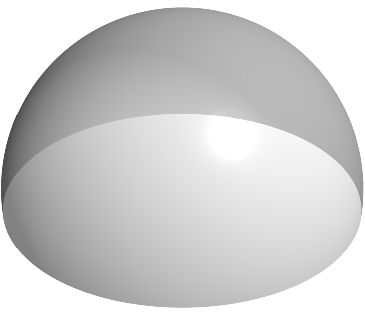
\includegraphics[width=2cm]{hemisphere.pdf}};
\draw  (.5,.75)--(.5,1.15);
\fill (.5,.75) circle (.8pt);
\fill (.5,1.15) circle (.8pt);
\end{tikzpicture}
\end{document}\\[4cm]
\documentclass[tikz]{standalone}
\usetikzlibrary{decorations.markings}
\begin{document}
\begin{tikzpicture}
\fill[draw=gray,gray!50] (0,0) circle (.5cm);
\begin{scope}[very thick,decoration={
    markings,
    mark=at position 0.5 with {\arrow{latex}}}
    ] 
%    \draw[postaction={decorate},thick,gray] (0,0) circle (1cm);
    \draw[rotate=90,postaction={decorate},thick,gray] (0,0) circle (.5cm);
%  \draw[rotate=180,postaction={decorate},thick,gray] (0,0) circle (1cm);
    \draw[rotate=270,postaction={decorate},thick,gray] (0,0) circle (.5cm);
\end{scope}
\end{tikzpicture}
\end{document}

\end{tabular}
\end{exampleAndImage}
\chapter{Fundamental Groups}\label{chapter:fundamental.groups}

\section{Homotopy}
Continuous maps \(f, g \colon X \to Y\) between topological spaces \(X, Y\) are \emph{homotopic}\define{homotopic} if there is a \emph{homotopy}\define{homotopy} between them, i.e. a map \(F \colon [0,1] \times X \to Y\), denoted by \(F_s(x)\) instead of \(F(s,x)\), so that \(F_0=f\) and \(F_1=g\).
If there is a subset \(X_0 \subset X\) on which \(f=g\), \(f\) is \emph{homotopic} to \(g\) \emph{relative}\define{homotopy!relative}\define{relative homotopy} to \(X_0\) if there is a homotopy \(F\) between \(f\) and \(g\) so that \(F_s\of{x}=f(x)\) for all \(x \in X_0\).
A map is \emph{null homotopic}\define{null homotopic} if it is homotopic to a constant map, i.e. a map whose image is a single point.
\begin{problem}{covering.spaces:homotopic}
Prove that the relation of being homotopic relative to some set is an equivalence relation.
\end{problem}
Given points \(x_0, x_1 \in X\), a \emph{path}\define{path} from \(x_0\) to \(x_1\) is a continuous map \(x \colon [0,1] \to X\) so that \(x(0)=x_0\) and \(x(1)=x_1\), i.e. a map \(x \colon \pr{[0,1],0,1} \to \pr{X,x_0,x_1}\).
We often omit to write the expression ``relative to \(\Set{0,1}\)'' when discussing homotopies of paths, and the reader will have to decide when we should have written that expression.

Intuitively, a homotopy between paths looks something like
\begin{center}
\documentclass[tikz]{standalone}
\usetikzlibrary{arrows,calc,shapes,decorations.pathreplacing}
\begin{document}
\begin{tikzpicture}[scale=.5]
%  \node at (0,0) {$F : I \times I \rightarrow X$};
\fill[gray] (6,0) circle (1.3pt);
  \node[label=below:$x_1$]  (x1) at (6,0)  {}; %{$\bullet$};
\fill[gray] (9,4) circle (1.3pt);
  \node[label=above:$x_0$]  (x0) at (9,4)  {}; % {$\bullet$};  
%  \node  at (9.5,2)  {$\subset X$}; 
  \draw[gray] (x1.center) to [out=5,in=-90]++(2.8,1.8) to[out=90,in=-95](x0.center);
  \draw[gray] (x1.center) to [out=10,in=-110]++(2.6,2) to[out=70,in=-103](x0.center); 
  \draw[gray] (x1.center) to [out=15,in=-105](x0.center);
  \draw[gray] (x1.center) to [out=30,in=-150](x0.center);
  \draw[gray] (x1.center) to [out=45,in=-170](x0.center); 
  \draw[gray] (x1.center) to [out=50,in=-105]++(1.2,3)to [out=75,in=-172](x0.center); 
  \draw[gray] (x1.center) to [out=55,in=-100]++(1.0,3) to[out=80,in=-175](x0.center); 
  \draw[gray] (x1.center) to [out=60,in=-90]++(0.8,3) to[out=90,in=-180] (x0.center);
%  \begin{scope}[every node/.style={draw, anchor=text, rectangle split,
%    rectangle split parts=7,minimum width=2cm}]
%    \node (R) at (2,4){ \nodepart{two} \nodepart{three}
%    \nodepart{four}$I\times I$\nodepart{five}\nodepart{six}\nodepart{seven}};
%  \end{scope}
%  \draw[decorate,decoration={brace,mirror,raise=6pt,amplitude=10pt}, thick]
%    (R.north west)--(R.south west) ;
%  \draw[decorate,decoration={brace,raise=6pt,amplitude=10pt}, thick]
%    (R.north east)--(R.south east); 
%  \draw[->] ($(R.west)+(-20pt,0)$) to[out=-180,in=240] ++(0,2)
%    to [out=60,in=120]node[above,midway]{$F(0,t_2)$}(x0) ; 
%  \draw[->] ($(R.north)+(0,10pt)$) to [out=60,in=120]
%    node[above,midway]{$\beta \simeq \alpha$} ++(4.5,-1) ; 
%  \draw[->] ($(R.east)+(20pt,0)$)  to [out=0,in=140]
%    node[right,midway]{$F(1,t_2)$}(x1) ; 
%  \draw[->] ($(R.south)+(0,-20pt)$)  to [out=-85,in=-30]
%    node[below,midway]{$\alpha$}++(7,0) ;    
\end{tikzpicture}
\end{document}

\end{center}
\begin{problem}{covering.spaces:reparam}
Take two paths \(x, y \colon [0,1] \to X\) for one is a \emph{reparameterisation},\define{reparameterisation} of the other, i.e. there is a continuous map \(\tau \colon [0,1] \to [0,1]\) so that \(y \circ \tau = x\) with \(\tau(0)=0\) and \(\tau(1)=1\).
Prove that \(x\) is homotopic to \(y\) relative to \(\Set{0,1}\).
\end{problem}
\begin{answer}{covering.spaces:reparam}
Let \(F_s(t)=x((1-s)t+s\tau(t))\).
\end{answer}
\begin{lemma}\label{lemma:pick.times}
Cover a topological space \(X\) in open sets \(X_a \subset X\).
Take a path \(x \colon [0,1] \to X\).
Then there are real numbers \(0=t_0 < t_1 < \dots < t_n=1\) so that \(x(t)\) stays in one open set \(X_{a_i}\) for \(t_i \le t \le t_{i+1}\).
\end{lemma}
\begin{proof}
Each point of \([0,1]\) lies in an open interval lying entirely inside one \(x^{-1}X_a\).
Replace that open interval with a smaller open interval: each point of \([0,1]\) lies in an open interval whose closure lies entirely inside one \(x^{-1}X_a\).
Since \([0,1]\) is compact, finitely many such open intervals cover \([0,1]\).
Take the endpoints of those intervals: \(0=t_0 < t_1 < \dots < t_n=1\).
\end{proof}

\section{Some inessential differential geometry}
Think of Euclidean space of dimension \(n\) as having \(n\) coordinates: 
\[
x=(x_1,\dots,x_n).
\]
An \(n\)-dimensional  \emph{manifold}\define{manifold} is a subset of Euclidean space \(\R{n+k}\), locally expressed as the graph of \(k\) of the coordinates as smooth functions of the other \(n\) coordinates.
An \(n\)-dimensional  \emph{manifold with corners}\define{manifold with corners} is a subset of Euclidean space \(\R{n+k}\), locally expressed as the graph of \(k\) of the coordinates as smooth functions of the other \(n\) coordinates, constrained to be inside an \(n\)-dimensional box.
A \emph{surface}\define{surface} is a \(2\)-dimensional manifold (perhaps with corners).
A continuous map of manifolds is \emph{smooth} if it is smooth as a map of those coordinates.
We won't prove:
\begin{theorem}
Every continuous map of manifolds is homotopic to a smooth map.
\end{theorem}
\begin{lemma}
Any path \(x \colon [0,1] \to M\) in a manifold (perhaps with corners) \(M\) is homotopic relative to \(\Set{0,1}\) to a smooth path.
\end{lemma}
\begin{proof}
If \(M=\R{n}\), and \(x \colon [0,1] \to M\) is a path then let \(y(t)=(1-t)x(0)+tx(1)\) and let \(F(s,t)=(1-s)x(t)+sy(t)\).
More generally, the same trick works for \(M\) any convex domain in \(\R{n}\), and in particular for \(M\) a box.

Suppose next that we have a path \(x(t)\) in a box \(M\), and we want to smooth out that path only inside some interval \(a < t < b\).
Take a smooth increasing function \(h(t)\) equal to \(0\) in a small neighborhood of \(a\), and equal to \(1\) in a small neighborhood of \(b\).
Let
\[
y(t) =
\begin{cases}
x(t), & \text{ if \(0 \le t \le a\)}, \\
(1-h(t))x(a)+h(t)x(b), & \text{ if \(a \le t \le b\)}, \\
x(t), & \text{ if \(b \le t \le 1\)}.
\end{cases}
\]
and let
\[
F(s,t)=(1-s)x(t)+sy(t).
\]

Cover \(M\) in open sets, each a graph over a convex open set in a box in \(\R{n}\).
Apply lemma~\vref{lemma:pick.times} to split \(x(t)\) into intervals on which it stays in these open sets.
On each interval, we use the first trick to smooth \(x\).
This done, \(x\) is now piecewise smooth.
We use the second trick near each corner to smooth out corners.
\end{proof}

\section{Loops}
A \emph{loop}\define{loop} is a path \(x \colon [0,1] \to X\) with \(x(0)=x(1)\).
Given a path \(x\) from \(x_0\) to \(x_1\) and a path \(y\) from \(x_1\) to \(x_2\), define a path \(x*y\) from \(x_0\) to \(x_2\) by
\[
(x*y)(t) =
\begin{cases}
x(2t), & \text{if \(0 \le t\le \frac{1}{2}\)}, \\
y(2t-1), & \text{if \(\frac{1}{2} \le t\le 1\)}.
\end{cases}
\]
and define \(\bar{x}(t)=x(1-t)\).
Also, for any point \(x_0\), define the null path \(x(t)=x_0\) for \(0 \le t \le 1\) which we just denote by \(x_0\).

If you have two paths and I have two paths, with homotopies fixing endpoints between your first and my first, and between your second and my second, then we can make a homotopy between paths glued together:
\begin{center}
\documentclass[tikz]{standalone}
\usetikzlibrary{arrows,calc,shapes,decorations.pathreplacing}
\begin{document}
\begin{tikzpicture}[scale=.5]
\fill[gray] (6,0) circle (1.3pt);
  \node[label=below:$x_0$]  (x1) at (6,0)  {}; % {$\bullet$};
  \fill[gray] (9,4) circle (1.3pt);
  \node[label=above:$x_1$]  (x0) at (9,4)  {}; % {$\bullet$};  
%  \node[label=above:$x_1$]  (x0) at (9,4)  {$\bullet$};  
  \draw[gray] (x1.center) to [out=5,in=-90]++(2.8,1.8) to[out=90,in=-95](x0.center);
  \draw[gray] (x1.center) to [out=10,in=-110]++(2.6,2) to[out=70,in=-103](x0.center); 
  \draw[gray] (x1.center) to [out=15,in=-105](x0.center);
  \draw[gray] (x1.center) to [out=30,in=-150](x0.center);
  \draw[gray] (x1.center) to [out=45,in=-170](x0.center); 
  \draw[gray] (x1.center) to [out=50,in=-105]++(1.2,3)to [out=75,in=-172](x0.center); 
  \draw[gray] (x1.center) to [out=55,in=-100]++(1.0,3) to[out=80,in=-175](x0.center); 
  \draw[gray] (x1.center) to [out=60,in=-90]++(0.8,3) to[out=90,in=-180] (x0.center);
\begin{scope}[shift={(3,4)}]
\fill[gray] (6,0) circle (1.3pt);
  \node%[label=below:$x_1$]  
  	(x1) at (6,0) {};%  {$\bullet$};
%  \node[label=above:$x_2$]  (x0) at (9,4)  {$\bullet$};  
\fill[gray] (9,4) circle (1.3pt);
  \node[label=above:$x_2$]  (x0) at (9,4)  {}; % {$\bullet$};  
  \draw[gray] (x1.center) to [out=5,in=-90]++(2.8,1.8) to[out=90,in=-95](x0.center);
  \draw[gray] (x1.center) to [out=10,in=-110]++(2.6,2) to[out=70,in=-103](x0.center); 
  \draw[gray] (x1.center) to [out=15,in=-105](x0.center);
  \draw[gray] (x1.center) to [out=30,in=-150](x0.center);
  \draw[gray] (x1.center) to [out=45,in=-170](x0.center); 
  \draw[gray] (x1.center) to [out=50,in=-105]++(1.2,3)to [out=75,in=-172](x0.center); 
  \draw[gray] (x1.center) to [out=55,in=-100]++(1.0,3) to[out=80,in=-175](x0.center); 
  \draw[gray] (x1.center) to [out=60,in=-90]++(0.8,3) to[out=90,in=-180] (x0.center);
\end{scope}
\end{tikzpicture}
\end{document}

\end{center}
Hence gluing paths together commutes with homotopy relative to \(\set{0,1}\).
\begin{problem}{covering.spaces:associative}
For any three paths \(x, y, z\), if \((x*y)*z\) is defined then so is \(x*(y*z)\), and vice versa, and they are homotopic relative to \(\Set{0,1}\).
\end{problem}
\begin{problem}{covering.spaces:inverse}
For any path \(x\), the path \(x*\bar{x}\) is homotopic to \(x(0)\)  relative to \(\Set{0,1}\) while \(\bar{x}*x\) is homotopic to \(x(1)\) relative to \(\Set{0,1}\).
\end{problem}
Therefore, for any topological space \(X\) and point \(x_0 \in X\), the homotopy classes of loops relative to \(\Set{0,1}\) form a group, called the \emph{fundamental group}\define{fundamental!group} of \(X\) and denoted \(\fundamentalGroup{X,x_0}\).\Notation{p1M}{\fundamentalGroup{X,x_0}}{fundamental group}

\begin{problem}{covering.spaces:conjugacy}
If \(x_0,x_1 \in X\) are two points connected by a path \(x\), then any loop \(y\) at \(x_0\) has an associated loop \(\bar{x} * \pr{y * x}\) at \({x_1}\). 
Prove that the homotopy class of \(\bar{x} * \pr{y * x}\) in \(\fundamentalGroup{X,x_0}\) depends only on the homotopy class of \(y\) in \(\fundamentalGroup{X,x_1}\), and that this gives an isomorphism of groups
\[
\fundamentalGroup{X,x_0} \to \fundamentalGroup{X,x_1}.
\]
\end{problem}

A topological space \(X\) is \emph{path connected}%
\define{path connected}%
\define{connected!path}
if any two points of \(X\) are the endpoints of a path in \(X\).
If \(X\) is path connected, then we usually ignore the point \(x_0\) and write \(\fundamentalGroup{X}\) instead of \(\fundamentalGroup{X,x_0}\), even though this is not strictly speaking well defined.
A path connected topological space \(X\) is \emph{simply connected}\define{simply connected}\define{connected!simply} if \(\fundamentalGroup{X}=\left\{1\right\}\).
\begin{example}
A \emph{star shaped set}\define{star shaped} is a set \(X \subset \R{n}\) so that there is some point \(x_0 \in X\) so that for every point \(x_1 \in X\), the line segment from \(x_0\) to \(x_1\) lies entirely in \(X\).
\begin{center}
\documentclass[border=10pt]{standalone}
\usepackage{pgfplots}
\pgfplotsset{compat=1.8}
\usepgfplotslibrary{polar}
\begin{document}
\begin{tikzpicture}
	\begin{polaraxis}[xtick=\empty,ytick=\empty,mark=none,draw=white,opacity=0,thin,width=3cm]
	\addplot+[mark=none,domain=0:360,samples=1000,draw=gray!50,fill=gray!20,opacity=1] 
		{2-sqrt(sqrt((abs(sin(3*x)))))+cos(9*x)*cos(9*x)*cos(9*x)*cos(9*x)}; 
	% the expression is the RADIUS
	\end{polaraxis}
\end{tikzpicture}
\end{document}

\end{center}
In other words, \(X\) admits the homotopy \(F \colon (s,x) \in [0,1] \times X \mapsto x_0+s\pr{x-x_0} \in X\).
Clearly \(\fundamentalGroup{X}=\Set{1}\) is the trivial group, where \(1\) is the constant path \(x_0\).
In particular, \(\fundamentalGroup{\R{n}}=\Set{1}\).
\end{example}
\begin{example}
For the circle \(S^1\), take any path \(z(t)=x(t)+iy(t))\) on \(S^1\) and write it as \(z(t)=e^{i\theta(t)}\) using trigonometry to prove that one can continuously pick out a value of \(\theta(t)\) for any continuous \(z(t)\).
The number 
\[
n(z) \defeq \frac{1}{2\pi} \pr{\theta(1)-\theta(0)}
\]
is an integer, since \(z\) is periodic.
Suppose that two loops \(z_0(t)\) and \(z_1(t)\) have the same values of \(n\of{z_0}=n\of{z_1}\) and start (and thus end) at the same point of \(S^1\), say at \(e^{i \alpha_0}\).
Pick continuous angles \(\theta_0(t), \theta_1(t)\) with \(\theta_0(0)=\theta_1(0)=\alpha_0\) and 
\[
z_0(t)=e^{i\theta_0(t)}, z_1(t)=e^{i \theta_1(t)}.
\]
Clearly 
\[
\theta_0(1)=\theta_1(1).
\]
Let
\[
\theta_s(t) = (1-s)\theta_0(t)+s\theta_1(t)
\]
and 
\[
z_s(t) = e^{i\theta_s(t)},
\]
a homotopy.
Therefore \(\fundamentalGroup{S^1}=\Z{}\), identifying the homotopy class of a loop \(z\) with the number \(n(z)\).
\end{example}
\begin{example}
For an annulus 
\[
A\defeq\Set{x \in \R{n}|r_0 < \norm{x} < r_1},
\]
the map 
\[
F_s(x)=\frac{x}{(1-s)+s\norm{x}}
\]
retracts the annulus to the unit sphere, and retracts paths on the annulus to those on the sphere, homotopies on the annulus to homotopies on the sphere, so that \(\fundamentalGroup{A}=\fundamentalGroup{S^{n-1}}\).
\end{example}
\begin{example}
It turns out to be more difficult to find the fundamental group of the plane punctured at two points, or at three points, etc.
\end{example}
\begin{example}
The spaces \(\R{}\) and \(\R{2}\) are not homeomorphic, as \(\R{}\) becomes path disconnected when we remove any point, while \(\R{2}\) does not.
\end{example}
\begin{example}
The spaces \(\R{2}\) and \(\R{3}\) are not homeomorphic, as \(\R{2}\) punctured at any point has fundamental group \(\Z{}\), while \(\R{3}\) punctured at any point remains simply connected.
\end{example}
\begin{exampleAndImage}{2cm}
The Hawaiian earring has a very complicated and uncountable fundamental group.
\tcblower
\documentclass[tikz]{standalone}
\begin{document}
\begin{tikzpicture}
\foreach \n in {1,2,...,100}{
	\draw[gray] ({1/\n},0) circle ({1/\n});
}
\end{tikzpicture}
\end{document}

\end{exampleAndImage}
\begin{example}
The union of all circles with irrational radius passing through the origin and tangent to the vertical axis is even more complicated than the Hawaiian earring.
\end{example}
\begin{lemma}
Any connected finite graph has finitely generated fundamental group.
\end{lemma}
\begin{proof}
Take a connected finite graph \(X\) and a vertex \(x_0 \in X\).
A \emph{tree}\define{tree} is a simply connected graph.
A \emph{maximal subtree}\define{maximal subtree} is a maximal simply connected subgraph; take one, say \(T \subset X\).
Then \(T\) contains all vertices, since otherwise we could add an edge that attaches one more vertex, without creating a loop (any loop would have two edges reaching that vertex).
Each path in \(X\) is determined up to homotopy by listing the edges it passes through.
Each path in \(T\) is uniquely determined, up to homotopy, by its end points, since there is then a unique list of edges giving a path between the end points. 
For each edge \(e_a\) of \(X\) not in \(T\), pick a loop \([x_a]\) in \(X\) starting at \(x_0\), and passing once along \(e_a\).
Every loop \([x]\) in \(X\), starting and ending at \(x_0\), passes finitely many times through each \(e_a\), either in the same direction or the opposite direction to \([x_a]\).
Picture the last edge \(e_a\) which \([x]\) passes along, and picture direction in which it passes.
We can suppose for simplicity that \([x_a]\) traverses \(e_a\) in the opposite direction.
Consider the loop \([y]=[x_a]*[x]\).
It goes through \(e_a\), say through the two vertices \(x_b,x_c\) of \(e_a\), and then passes through \(T\) to \(x_0\), and then back again to \(x_b\) and then \(x_c\).
By uniqueness of paths in \(T\), up to homotopy, with given end points, we can arrange that \([y]\) takes the same route from \(x_c\) to \(x_0\) and then back again.
So \([y]\) is homotopic to cutting that part of \([y]\) out, i.e. up to homotopy \([x_a][x]\) has one fewer pass through \(e_a\) that \([x]\) did.
By induction, we arrange that \([x]\) is a product of these various \([x_a]\).
\end{proof}
\begin{lemma}
Any graph with countably many vertices and edges has countable fundamental group.
\end{lemma}
\begin{proof}
By compactness of \([0,1]\), each loop in the graph can only hit finitely many vertices and so finitely many edges.
Listing the vertices and edges of the loop in order gives the loop up to homotopy.
\end{proof}

\section{More inessential remarks on differential geometry}
A \emph{diffeomorphism}\define{diffeomorphism} is a smooth of manifolds with smooth inverse.
We will not prove:
\begin{theorem}[Sard]
Take a smooth map \(\varphi \colon P \to Q\) of manifolds.
If \(P\) has smaller dimension than \(Q\), then the image of \(\varphi\) is nowhere dense.
If \(P\) and \(Q\) have  equal dimension, there is a dense set of points \(q_0\in Q\) whose preimage \(\varphi^{-1}\set{q_0}\) consists entirely of points \(p_0\in P\) near which \(\varphi\) is a local diffeomorphism.
\end{theorem}
Careful: this point \(q_0\) could have empty preimage, for example if \(\varphi\) maps all of \(P\) to a single point of \(Q\).
\begin{example}
For the spheres \(S^2, S^3, \dots\), any path \(x \colon [0,1] \to S^n\) is smoothly approximated by some smooth path \(y \colon [0,1] \to \R{n+1}\) homotopic to \(x\), which we then divide by \(\norm{y}\) to get a smooth path homotopic to \(x\) lying in \(S^n\).
By Sard's theorem, \(y\) misses some point of the sphere.
Recall that stereographic projection from that point identifies the rest of the sphere with \(\R{n}\), where we can use our previous result to homotope to a constant map: \(\fundamentalGroup{S^n}=\Set{1}\).
Note that this doesn't work for the circle \(S^1\), where the application of Sard's theorem doesn't tell us anything.
\end{example}
A more difficult theorem, which we won't prove, but which may provide some comfort:
\begin{theorem}[Whitney \cite{Hirsch:1994} p. 49 Theorem 2.6]
The smooth maps between any two manifolds are dense in the continuous maps, in the topology of uniform convergence on compact sets, and every continuous map is homotopic to a smooth map.
\end{theorem}

\section{Maps and fundamental groups}
A \emph{diagram}\define{diagram} is a collection of maps between sets, drawn as a graph like:
\[
\begin{tikzcd}[column sep=small, row sep=small]
X \arrow[rr,"f"] \arrow[dr,"g"] & & Z \arrow[dl,"h"] \\
{} & Y & {}
\end{tikzcd}
\]
Start at one of the sets, and follow a path along the maps, in the direction of their arrows: compose those maps.
The diagram \emph{commutes}\define{commutative!diagram}\define{diagram!commutative} if any two paths with the same starting and ending points give the same composition.
In our example, this means that \(g=h \circ f\).

\begin{lemma}
A continuous map \(f \colon X \to Y\) between topological spaces yields a group morphism
\[
f_* \colon \fundamentalGroup{X,x_0} \to \fundamentalGroup{Y,y_0}
\]
where \(y_0=f\of{x_0}\), given by
\[
f_* [x]=[f \circ x]
\]
for any path \(x \colon [0,1] \to X\).
The group morphism doesn't change if \(f\) varies through a homotopy of maps taking \(x_0\) to \(y_0\).
More generally, if we take homotopy \(f_t\) of \(f\) through a family of maps taking, say \(x(t)\) to \(y(t)\), for some paths \(x(t), y(t)=f_t\of{x(t)}\), then there is a commutative diagram between the maps \(f_{0*}\) and \(f_{1*}\):
\[
\begin{tikzcd}
\fundamentalGroup{X,x_0} \arrow{r}{f_0} \arrow{d}{x_*} & \fundamentalGroup{Y,y_0} \arrow{d}{y_*} \\
\fundamentalGroup{X,x_1} \arrow{r}{f_1} & \fundamentalGroup{Y,y_1}
\end{tikzcd}
\]
Under composition of continuous maps
\[
\begin{tikzcd}
X \arrow{r}{f}  & Y \arrow{r}{g} & Z
\end{tikzcd}
\]
the group morphisms 
\[
\begin{tikzcd}
\fundamentalGroup{X,x_0} \arrow{r}{f}  & \fundamentalGroup{Y,y_0} \arrow{r}{g} & \fundamentalGroup{Z,z_0}
\end{tikzcd}
\]
compose: \(\pr{g \circ f}_* = g_* \circ f_*\).
\end{lemma}

A \emph{homotopy equivalence}\define{homotopy!equivalence} is a continuous map \(f \colon X \to Y\) between topological spaces so that there is a continuous map \(g \colon Y \to X\) for which \(f \circ g\) and \(g \circ f\) are both homotopic to identity maps.
A homotopy equivalence identifies fundamental groups.
\begin{example}
The annulus in \(\R{n}\) is homotopy equivalent to the unit sphere, by the map including the sphere into the annulus.
\end{example}
\begin{example}
The sphere in \(\R{n}\) punctured at one point is homotopy equivalent to \(\R{n-1}\) by Ptolemaic projection, and so homotopy equivalent to a point.
\end{example}
\begin{example}
The sphere in \(\R{n}\) punctured at two points is homotopy equivalent to the annulus in \(\R{n-1}\) by Ptolemaic projection, and so to the sphere in \(\R{n-1}\).
\end{example}
\begin{example}
If \(L \subset \R{3}\) is a line, the topological space \(X=\R{3}-L\) is homotopy equivalent to \(S^1\), by projecting to a plane perpendicular to \(L\), punctured where the plane strikes \(L\), and then taking a homotopy to a circle.
\end{example}
\begin{theorem}[Fundamental theorem of algebra]\define{theorem!fundamental, of algebra}\define{algebra!fundamental theorem of}\define{fundamental!theorem of algebra}
Every nonconstant polynomial function of one complex variable has a complex root.
\end{theorem}
\begin{proof}
Take a nonconstant polynomial function 
\[
p(z)=a_0 + a_1 z + \dots + a_n z^n,
\]
with \(a_n \ne 0\).
Clearly \(p(z)\) has a root just where \(p(z)/a_n\) has a root, so we can assume that \(a_n=1\).
Let \(\alpha\) be the maximum of \(|a_0|, |a_1|, \dots, |a_{n-1}|\).
If we pick any \(z\) with \(|z|>(n-1)\alpha\) then clearly the leading term of \(p(z)\) is larger than all other terms added together, so \(p(z) \ne 0\).
Rescale the \(z\) variable if needed to ensure that \((n-1)\alpha<1\).
So if \(|z| \ge 1\) then \(p(z) \ne 0\).
By the same reasoning, none of the functions
\[
p_t(z) = z^n + (1-t)\pr{a_0 + a_1 z + \dots + a_{n-1} z^{n-1}},
\]
vanishes as long as \(|z|\ge 1\), a homotopy betweeen \(p_0(z)=p(z)\) and \(p_1(z)=z^n\).
Let
\[
g_t(e^{i\theta})=\frac{p_t(z)}{p_t(1)},
\]
where \(z=e^{i \theta}\), for \(0 \le t \le 1\).
This map is a homotopy between the loop 
\[
g_0(z) = \frac{p(z)}{p(1)}
\]
with \(z=e^{i\theta}\) and the loop 
\[
g_1(z)=z^n.
\]
Note that \(g_t(1)\) is fixed during the homotopy.

Let
\[
f_t(z)=\frac{p(tz)}{p(t)},
\]
where \(z=e^{i \theta}\) and \(0 \le t \le 1\).
The map \(f\) is a homotopy from the trivial loop at \(t=0\) to a loop at \(t=1\):
\[
f_1(z) =\frac{p(z)}{p(1)} = g_0(z),
\]
for \(z=e^{i\theta}\).
So, inside the plane punctured at the origin, the trivial loop is homotopic to the loop winding \(n\) times and so \(n=0\).
\end{proof}
\begin{problem}{covering.spaces:product.grp}
Prove that the fundamental group of a product is the product of the fundamental groups:
\[
\fundamentalGroup{X \times Y, \pr{x_0,y_0}}
\cong
\fundamentalGroup{X, x_0}
\times
\fundamentalGroup{Y, y_0}.
\]
\end{problem}
\begin{example}
The torus \(T^n=S^1 \times S^1 \times \dots \times S^1\) has fundamental group
\[
\fundamentalGroup{T}=\Z{n}.
\]
\end{example}
\begin{problem}{covering.spaces:horned.sphere}
Give some explanation (not a rigorous proof) why the surface called \emph{Alexander's horned sphere}\define{Alexander's horned!sphere} has uncountable fundamental group, while the open subset of \(\R{3}\) inside (called \emph{Alexander's horned ball}\define{Alexander's horned!ball}) is simply connected.
\begin{center}
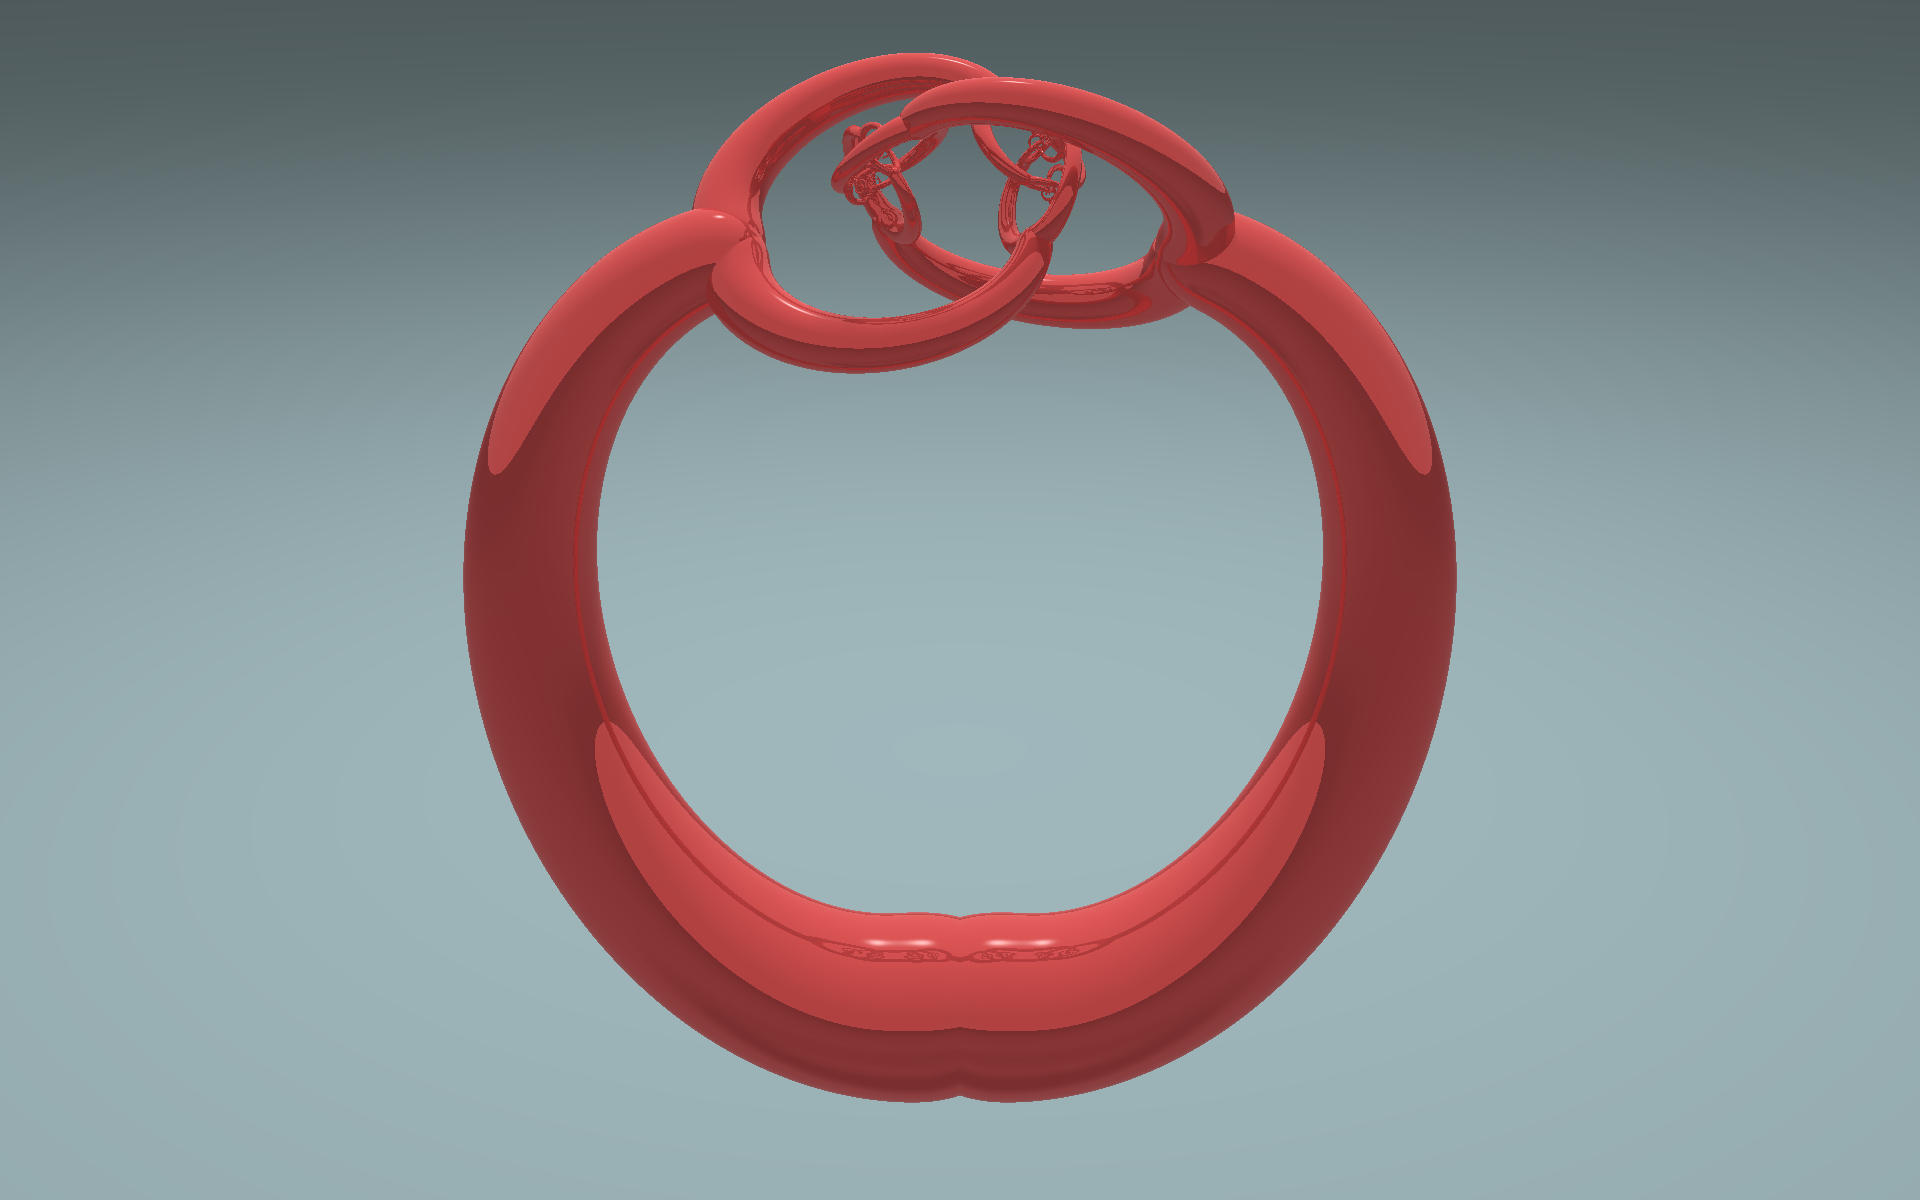
\includegraphics[width=\textwidth]{horned-sphere}
\cprotect\legend{Alexander's horned sphere, Krzysztof Rykaczewski}
\end{center}
\end{problem}
\begin{corollary}\label{corollary:manifolds.countable.pi.1}
If a path connected topological space \(X\) admits a countable basis of simply connected open sets, then its fundamental group is countable.
\end{corollary}
\begin{proof}
The homotopy class of any path is determined by listing off finitely many simply connected open sets that cover it, in the order that it enters them, as in lemma~\vref{lemma:pick.times}.
\end{proof}
\begin{corollary}
Every compact and locally simply connected topological space \(X\) has finitely generated fundamental group.
\end{corollary}
\begin{proof}
By compactness, we can find a finite covering by simply connected open sets \(X_a\) and cover the overlaps \(X_a \cap X_b\) by finitely many path connected open sets \(X'_c\).
The homotopy class of any path is determined by listing off finitely many simply connected open sets that cover it, in the order that it enters them, as in lemma~\vref{lemma:pick.times}.
The homotopy class of any path is determined by listing off finitely many \(X_a\) and \(X'_c\) that cover it, in the order it enters them, as in lemma~\vref{lemma:pick.times}.
\end{proof}

\chapter{Covering spaces}\label{chapter:covering.spaces}

\section{Covering maps}
A continuous map \(f \colon X \to Y\) of topological spaces \emph{evenly covers}\define{evenly covered}
an open set \(U_Y \subset Y\) if \(f^{-1}U_Y \subset X\) is a disjoint union of open sets mapped homeomorphically to \(U_Y\) by \(f\), called \emph{sheets}\define{sheet}.
The map \(f \colon X \to Y\) is a \emph{covering map}\define{covering map} if \(Y\) has an open cover by evenly covered open sets.
A \emph{covering space} of a topological space \(Y\) is a topological space \(X\) equipped with a covering map \(f \colon X \to Y\). 
Covering spaces are the main tool to calculate fundamental groups.
\begin{exampleAndImage}{3cm}
The map \(\theta \in \R{} \mapsto \pr{\cos \theta, \sin \theta} \in S^1\) is a covering map.
Every open set of \(S^1\) which is not all of \(S^1\) is evenly covered: use trigonometry to write out an angle \(\theta\) for each point of your open set, well defined and unique up to adding \(2\pi\) multiples.
The sheets correspond to the \(2\pi\) multiples.
\tcblower
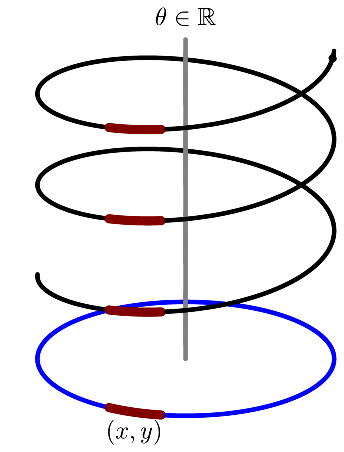
\includegraphics[width=3cm]{circle-covering}
\end{exampleAndImage}
\begin{example}
The map \(e^{i \theta} \in S^1 \mapsto e^{i n \theta} \in S^1\) is an \(n\)-sheeted covering.
\end{example}
\begin{example}
The map \(x \in \R{n} \mapsto \pr{e^{ix_1}, e^{ix_2}, \dots e^{ix_n}}\) is a covering map of the \(n\)-dimensional torus \(T^n\defeq S^1 \times S^1 \times \dots \times S^1\).
\end{example}
\begin{example}
The map \(x \in S^2 \mapsto [x] \in \RP{2}\) taking a point to the line through that point is a 2-sheeted covering of the projective plane.
\end{example}
\begin{example}
Take a manifold \(M\).
Let \(\hat{M}\) be the set of pairs \((m,o)\) where \(m \in M\) and \(o\) is an orientation of \(T_m M\), i.e. a choice of oriented basis up to equivalence, with two bases equivalent if the change of basis matrix between them has positive determinant.
Then \(\hat{M} \to M\) is a 2-1 covering map.
If \(M\) is orientable, then \(\hat{M}\) is a disjoint union of two copies of \(M\) and the covering map is a homeomorphism on each copy.
If \(M\) is not orientable, then \(\hat{M}\) is connected.
\end{example}
\begin{problem}{covering.spaces:zero.three}
Let \(X\) be the open interval \((0,3) \subset \R{}\).
Let \(Y\) be the unit circle in the complex plane.
Prove that the map \(f \colon X \to Y\) given by \(f(x)=e^{2\pi ix}\) is not a covering map.
\end{problem}
\begin{answer}{covering.spaces:zero.three}
Suppose that \(U_Y \subset Y\) is an evenly covered open set near \(1 \in Y\).
Write each point of \(Y\) as \(w = u+iv \in Y\).
Then \(U_Y\) contains a connected open set near \(1 \in Y\), say the ``interval'' \(-\varepsilon < v < \varepsilon\).
Since \(U_Y\) is evenly covered, so is this ``interval''.
The preimage of this ``interval'' is a union of 4 open intervals: 
\[
(0,\delta) 
\cup (1-\delta,1+\delta)
\cup (2-\delta,2+\delta)
\cup (3-\delta,3)
\]
where 
\[
\delta = \frac{\sin^{-1} \varepsilon}{2 \pi}.
\]
Any sheet over our open set is homeomorphic so also path connected, so lies inside one of these 4 intervals.
But no open subset of the first interval maps onto our ``interval'' as the map takes on values \(u+iv\) with \(0 < v < \varepsilon\) there.
\end{answer}
\begin{exampleAndImage}{6.63cm}
In the complex plane \(\C{}\), the map \(z \in \C{}-\set{0} \mapsto z^3 \in \C{}-\set{0}\) is a covering map.
We like to pretend that we can draw every covering map as a picture of ``sheets'', but in this case the best picture we get is an immersed surface.
\tcblower
\documentclass[tikz]{standalone}
\begin{document}
\begin{tikzpicture}
\clip (-4.03,-7.22) rectangle (2.6,5.15);
\fill[gray!25] (-.8,-6.2) ellipse (3.2cm and 1cm);
\fill[white,draw=gray] (-.8,-6.2) ellipse (.08cm and .025cm);
\node at (0,0) {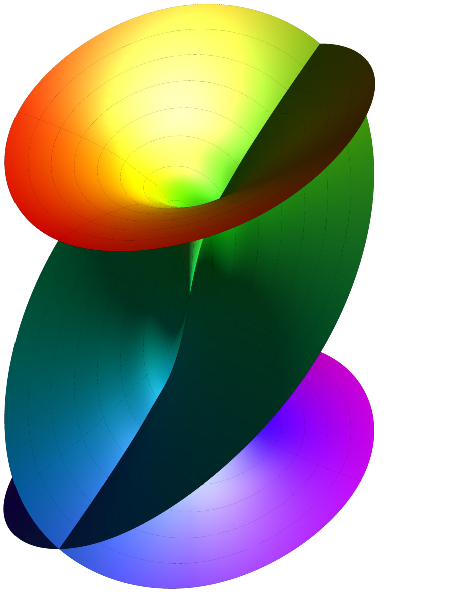
\includegraphics[width=8cm]{complex-cube-root-graph-3}};
\end{tikzpicture}
\end{document}
\end{exampleAndImage}
\begin{problem}{covering.spaces:define.sheetedness}
Prove that the number \(n\) of sheets (which might be \(\infty\)) above an evenly covered open set is constant along any path in \(Y\).
In particular, if \(Y\) is path connected, this number \(n\) is constant, and we say that the covering map is \(n\) to \(1\).
\end{problem}
The \emph{fiber}\define{fiber} of a map \(f \colon X \to Y\) over a point \(y_0 \in Y\) is the set \(f^{-1}\set{y_0}\), usually denoted \(X_{y_0}\).
\begin{problem}{covering.spaces:discrete.fiber}
Prove that \(X_{y_0} \subset X\) is discrete, i.e. has the discrete topology as a subset of \(X\).
\end{problem}
\begin{answer}{covering.spaces:discrete.fiber}
Pick an evenly covered open set \(U_{y_0} \subset Y\) containing \(y_0\).
Every point \(x_0 \in X_{y_0}\) lies in a sheet, say \(U_{x_0}\), over \(U_{y_0}\).
Take two distinct points \(x_0, x_1 \in X_{y_0}\).
The sheets \(U_{x_0}\) and \(U_{x_1}\) are disjoint so \(x_1\) is not in \(U_{x_0}\) and \(x_0\) is not in \(U_{x_1}\).
Hence \(X_{y_0} \cap U_{x_0} = \set{x_0}\).
Take any subset \(S \subset X_{y_0}\).
Then 
\[
S = X_{y_0} \cap \bigcup_{x \in S} U_{x} 
\]
is the intersection of \(X_{y_0}\) with an open subset 
\[
\bigcup_{x \in S} U_{x} \subset X,
\]
so is open inside \(X_{y_0}\).
\end{answer}
\begin{problem}{covering.spaces:Hausdorfficity}
Suppose that \(f \colon X \to Y\) is a covering map.
Prove \(X\) is Hausdorff if and only if \(Y\) is Hausdorff.
\end{problem}
\begin{answer}{covering.spaces:Hausdorfficity}
Suppose that \(Y\) is Hausdorff. 
Take distinct points \(x_1, x_2\) of \(X\).
Let \(y_1=f(x_1)\) and \(y_2=f(x_2)\).

Suppose that \(y_1 \ne y_2\).
Take disjoint open sets \(U_1, U_2 \subset Y\) so that \(y_1 \in U_1\) and \(y_2 \in U_2\).
Then \(f^{-1}U_1, f^{-1}U_2 \subset X\) are disjoint open sets so that \(x_1 \in f^{-1}U_1\) and \(x_2 \in f^{-1}U_2\).

Suppose that \(y_1 = y_2\).
Take an evenly covered open set \(U \subset Y\) containing \(y_1\).
Every point \(x_1 \in X_{y_0}\) lies in a sheet, say \(U_{x_1}\), over \(U\).
The sheets \(U_{x_1}\) and \(U_{x_2}\) are disjoint open sets.

Now instead suppose that \(X\) is Hausdorff.
Take distinct points \(y_1, y_2\) in \(Y\).
Take two points \(x_1, x_2\) in \(X\) so that \(y_1=f(x_1)\) and \(y_2=f(x_2)\).
Pick evenly covered open sets \(U_{y_1}\) and \(U_{y_2}\) around \(y_1\) and \(y_2\).
Pick disjoint open sets \(W_{x_1}\) and \(W_{x_2}\) around \(x_1\) and \(x_2\).
Let \(U_{x_1}=W_{x_1} \cap f^{-1} U_{y_1}\).
Then \(f\) is a homeomorphism of \(U_{x_1}\) to its image inside \(U_{y_1}\); call its image \(V_{y_1}\).
Similarly define \(V_{y_2}\).
Because \(f\) homeomorphically maps \(U_{x_1}\) to \(V_{y_1}\), \(V_{y_1}\) is an open set in \(Y\).
The sets \(V_{y_1}\) and \(V_{y_2}\) are disjoint since they are images of disjoint open sets in \(X\).
\end{answer}
\begin{problem}{covering.spaces:compact}
Prove that every proper local diffeomorphism \(f \colon P \to Q\) between manifolds without boundary, with \(Q\) connected, is a covering map.
\end{problem}
\begin{answer}{covering.spaces:compact}
Take a point \(q_0\in Q\).
Because \(f\) is proper, the fiber \(P_{q_0} \defeq f^{-1}\Set{q_0}\) is compact.
Because \(f\) is a local diffeomorphism, each point \(p_0 \in P_{q_0}\) lies in an open set \(U_{p_0} \subset P\) taken by \(f\) diffeomorphically to a neighborhood  \(U_{q_0} \subset Q\).
The set \(P_{q_0}\) intersects \(U_{p_0}\) in a set taken by \(f\) to \(\Set{q_0}\), so just the single point \(p_0\).
Therefore every point \(p_0 \in P_{q_0}\) lies an open set \(U_{p_0}\) containing only \(p_0\), so \(P_{q_0}\) is a discrete set of points.
Being compact, \(P_{q_0}\) is therefore a finite set of points, say
\[
P_{q_0} = \Set{p_1, p_2, \dots, p_n},
\]
with each point \(p_j\) lying in an open set \(U_{p_j}\) taken diffeomorphically to some open set 
\[
f\of{U_{p_j}} \subset Q
\]
around \(q_0\).
Since there are finitely many such open sets, their intersection is open; call it \(U_{q_0}\).
Then replace \(U_{p_j}\) by
\[
U_{p_j} \cap f^{-1}U_{q_0} 
\]
so we can arrange that \(f\) takes each of the open sets 
\[
U_{p_1}, U_{p_2}, \dots, U_{p_n}
\]
diffeomorphically to \(U_{q_0}\).
\end{answer}
\begin{theorem}[Fundamental theorem of algebra]\define{theorem!fundamental, of algebra}\define{algebra!fundamental theorem of}\define{fundamental!theorem of algebra}
Suppose that \(k\) is a field containing \(\R{}\) and of finite dimension as a real vector space.
Then \(k=\R{}\) or \(k=\C{}\), up to isomorphism.
In particular, the splitting field of any real or complex polynomial is \(\R{}\) or \(\C{}\), i.e. every complex polynomial in one variable splits into a product of linear factors over \(\C{}\).
\end{theorem}
\begin{proof}
Pick any inner product on the real vector space \(k\).
Take the unit sphere \(S \subset k\).
The map \(f \colon x \in S \mapsto x^2/|x^2| \in S\) is smooth.
Compute that
\[
f'(x)y=\frac{2x}{|x^2|}\pr{y-\ip{f(x)}{xy}x}.
\]
In particular, if \(f'(x)y=0\) then \(y\) is a scalar multiple of \(x\).
So for \(y\) tangent to \(S\), \(f'(x)y=0\) just when \(y=0\), i.e. \(f\) is a local diffeomorphism.
The sphere is compact, so \(f \colon S \to S\) is a covering map.
If \(f(x)=f(y)\), pick a real number \(\lambda > 0\) so that \(\lambda^2=|x^2|/|y^2|\).
Check that \((x-\lambda y)(x+\lambda y)=0\), so \(x=\pm \lambda y\), i.e. up to scaling \(x=\pm y\), so \(f \colon S \to S\) is 2-1.
But the sphere of dimension \(2\) or more is simply connected, so does not admit a covering map of degree \(2\) from a connected space.
So \(S\) is the \(0\)-dimensional or \(1\)-dimensional sphere, i.e. \(k=\R{}\) or \(k\) is a \(2\)-dimensional real algebra.
Suppose that \(k\) is \(2\)-dimensional.
Pick some \(y \in k\) nonzero.
Then \(y/|y|\) lies in the image of \(f\), i.e., for some \(x\) with \(|x|=1\), 
\[
\frac{x^2}{|x^2|}=\frac{y}{|y|}.
\]
So if we let
\[
\lambda = \sqrt{\frac{|y|}{|x^2|}},
\]
and replace \(x\) by \(\lambda x\), we find \(x^2=y\).
So every nonzero element of \(k\) has a square root, and so in particular, \(-1 \in \R{}\) has a square root in \(k\), so \(k\) contains \(\C{}\), and hence \(k=\C{}\).
Note that we could pick \(k\) to be the splitting field of any real or complex polynomial.
\end{proof}
\begin{exampleAndImage}{5cm}
The \emph{harmonic archipelago} is given by drawing the Hawaiian earring on the plane, and then raising up the plane to a hollow hill, of unit height, between each successive pair of rings, with diameter of each hill becoming successively smaller approaching zero.
The limits of the hilltops are not in the archipelago, so it is not compact.
We can continuously deform any loop, based at the limit point of those hills, around finitely many hills in finite time, but not around all of them, since a map from a compact set has compact image.
The fundamental group is very complicated.
The set of points to the right of some line in our picture is homeomorphic to disk, so identified with a disk in any connected covering space.
Every connected covering space is thus a homeomorphism.
Wild Topology, Creative Commons Attribution 4.0 International License.
\tcblower
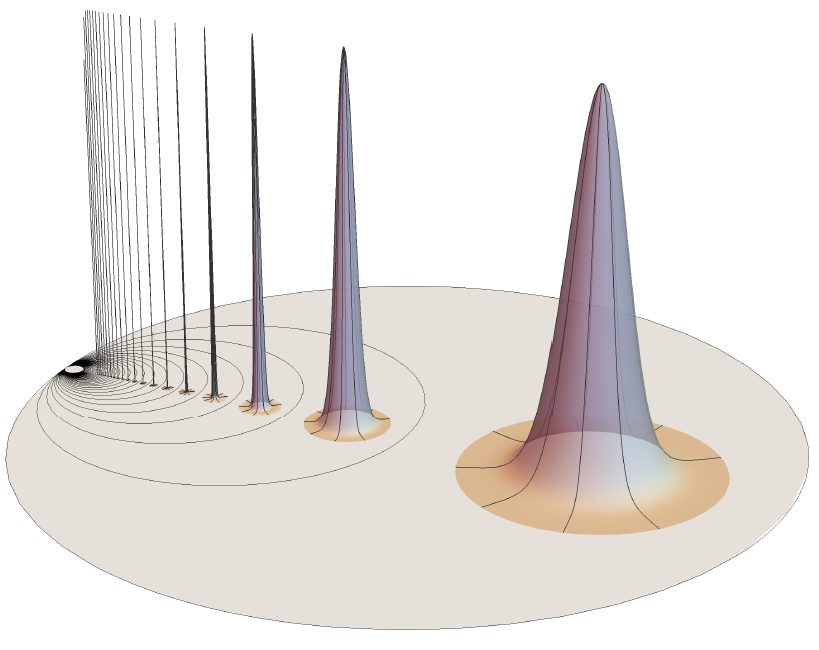
\includegraphics[width=5cm]{ha}
\end{exampleAndImage}

\section{Quotients by group actions}
An \emph{action}%
\define{group!action}%
\define{action!group}
of a group \(\Gamma\) on a topological space \(X\) is a map associating to each \(g \in \Gamma\) a continuous map \(X \to X\) denoted \(x \mapsto gx\) or sometimes denoted \(x \mapsto g \cdot x\), so that \(g(hx)=(gh)x\) for any \(g, h \in \Gamma\) and \(x \in X\) and so that \(1x=x\) for any \(x \in X\).
The action is \emph{free}\define{free!group action}\define{action!group!free}\define{group!action!free} if for any \(x \in X\), the only \(g \in \Gamma\) for which \(gx=x\) is \(g=1\).
The action is a \emph{covering action}%
\define{covering!group action}%
\define{action!covering}%
\define{group! action!covering} 
if any \(x \in X\) lies in an open set \(U \subset X\) so that the only \(g \in \Gamma\) for which \(gU\) intersects \(U\) is \(g=1\).
A group action is \emph{proper}%
\define{proper!group action}%
\define{group!action!proper}%
\define{action!group!proper}
when any points \(x, y \in X\) lie in open sets \(U_x, U_y\) so that \(gU_x\) intersects \(U_y\) for only finitely many \(g \in \Gamma\).
The \emph{orbit}\define{orbit} of a point \(x \in X\) is the set \(\Gamma x\defeq \set{gx|g \in \Gamma}\).
The \emph{quotient space}%
\define{quotient!space}%
\define{space!quotient}
\(X/\Gamma\) of the group action is the set of orbits, with the \emph{quotient map} \(x \in X \mapsto \Gamma x \in X/\Gamma\).
\begin{problem}{covering.spaces:prop.disc.metric}
Suppose that \(X\) is a metric space and that \(\Gamma\) acts on \(X\) by isometries.
Prove that \(\Gamma\) acts on \(X\) as a covering action if and only if the action is free with discrete orbits.
\end{problem}
\begin{problem}{covering.spaces:not.proper.disc}
Take an invertible matrix \(A\) with at least one eigenvalue \(\lambda\) satisfying \(\lambda > 1\) and at least one eigenvalue \(\mu\) satisfying \(0 < \mu < 1\).
Let \(M\defeq \R{n}-\set{0}\) and let \(\Gamma\defeq\set{A^n|n \in \Z{}}\).
Show that the action of \(\Gamma\) on \(M\) has discrete orbits, but the quotient space is not Hausdorff.
\end{problem}
\begin{problem}{covering.spaces:compact.quot}
If a group \(\Gamma\) acts on a topological space \(X\) and
\(X\) contains a compact set intersecting every \(\Gamma\)-orbit, then \(\bar{X}\) is also compact.
\end{problem}
\begin{theorem}\label{theorem:quotient.properly.discont}
Take a group \(\Gamma\) acting on a topological space \(X\).
The quotient map \(X \to \bar{X}= X/\Gamma\) is a covering map just when the action is a covering action.
\end{theorem}
\begin{proof}
For each point \(x \in X\) pick some open set \(U_x \subset X\) containing \(x\) so that \(gU_x\) doesn't intersect \(U_x\) for any \(g \in \Gamma\) unless \(g=1\).
The image \(\bar{U}_x \subset \bar{X}\) has preimage in \(X\) precisely the union of the nonoverlapping translates \(gU_x\) for \(g \in \Gamma\).
The open sets in \(\bar{U}_x\) have preimages precisely the \(\Gamma\)-invariant open sets in the translates of \(U_x\), precisely one of which lies in \(U_x\).
Hence the quotient map restricted to \(U_x\) is a homeomorphism \(U_x \to \bar{U}_x\).
Each element of \(\Gamma\) interchanges the sheets.
Conversely, if the quotient map is a covering map, then evenly covered open sets have preimages precisely open sets \(U\) not intersecting their translates \(gU\).
\end{proof}
\begin{theorem}\label{theorem:inv.open.sets}
Take an action of a group \(\Gamma\) on a Hausdorff space \(X\).
The quotient space is Hausdorff just when any two points of \(X\) lie in disjoint \(\Gamma\)-invariant open sets.
\end{theorem}
\begin{proof}
Take two points \(\bar{x}\ne \bar{y} \in \bar{X}\) in the quotient space \(\bar{X}\defeq X/\Gamma\).
Take points \(x, y \in X\) mapping to them.
If \(\bar{x}, \bar{y}\) lie in disjoint open sets \(\bar{U}_{\bar{x}}, \bar{U}_{\bar{y}}\), then the preimages of these open sets are disjoint \(\Gamma\)-invariant open sets around \(x\) and \(y\).

Conversely, take any disjoint \(\Gamma\)-invariant open sets around \(x\) and \(y\), \(U_x, U_y\).
Let \(\bar{U}_{\bar{x}}, \bar{U}_{\bar{y}}\) be their images in \(\bar{X}\).
By \(\Gamma\)-invariance, the preimage of \(\bar{U}_{\bar{x}}\) is \(U_x\) so \(\bar{U}_{\bar{x}}\) is open and \(\bar{U}_{\bar{x}} \cap \bar{U}_{\bar{y}}\) has preimage \(U_x \cap U_y\) empty so is empty.
\end{proof}
\begin{theorem}\label{theorem:proper.action}
Any proper group action on any Hausdorff space has Hausdorff quotient space.
\end{theorem}
\begin{proof}
Surround points \(x, y \in X\) with open sets \(U_x, U_y\) so that \(gU_x\) is disjoint from \(U_y\) except for finitely many \(g \in \Gamma\), say \(g_1, g_2, \dots, g_n\).
Because \(X\) is Hausdorff, for each \(j\) we can take ``houses'': disjoint open sets \(V_j, W_j\) so that \(V_j \subset g_j U_x\) and \(W_j \subset U_y\) and \(g_j x_j \in U_j\) and \(y \in W_j\).
Replace \(U_x\) with
\[
\bigcap_j g_j^{-1} U_j
\]
and \(U_y\) with
\[
\bigcap_j W_j.
\]
The resulting sets \(U_x\) and \(U_y\) have all translates disjoint, i.e. \(x\) and \(y\) lie in disjoint invariant open sets.
\end{proof}
A group \(\Gamma\) acting on a metric space \(X\) acts \emph{by isometries}%
\define{action!group!by isometries}%
\define{isometry!action}%
\define{group!action!by isometries}
if \(x \mapsto gx\) is an isometry for all \(g \in \Gamma\), i.e. \(d(gx,gy)=d(x,y)\) for any points \(x,y\) and \(g \in \Gamma\).
\begin{theorem}\label{theorem:metric.quotient}
Take a group action on a metric space \(X\) by a group of isometries \(\Gamma\).
The following are equivalent:
\begin{enumerate}
\item
The orbits are closed.
\item
Any two points of \(X\) lie in disjoint \(\Gamma\)-invariant open sets.
\item
The quotient space is a metric space, under the quotient metric
\[
d(\bar{x},\bar{y})=\inf_{g \in \Gamma} d(gx,y),
\]
so that the metric space topology agrees with the quotient topology.
\end{enumerate}
\end{theorem}
\begin{proof}
The orbits are closed just when any point in any orbit lies at a positive minimum distance from some point in any other chosen orbit, which occurs just when the ``quotient metric'' expression \(d\) is a metric.

Suppose that the orbits are closed.
Then the balls around distinct points \(\bar{x},\bar{y} \in \bar{X}\) have as preimages in \(X\) some disjoint \(\Gamma\)-invariant open sets.

Suppose that any two points \(x \ne y \in X\) lie in disjoint \(\Gamma\)-invariant open sets \(U_x, U_y\).
It is clear that the expression \(d\) above is continuous on \(\bar{X} \times \bar{X}\), since any open set of real numbers has open preimage inside \(X \times X\).
Next we want to prove that \(d(\bar{x},\bar{y})=0\) just when \(\bar{x}=\bar{y}\).
If \(d(g_j x, y) \to 0\) for some \(g_j \in \Gamma\), then \(g_j x\) enters \(U_y\) for all but finitely many \(j\), and so \(U_x \cap U_y\) is not empty.

So \(d\) is a metric on \(\bar{X}\).
If \(x \in X\) maps to \(\bar{x} \in \bar{X}\) then the ball of radius \(r\) around each point \(\bar{x}\) has preimage precisely the set of points \(y \in X\) so that \(d(gy,x)<r\) for some \(g \in \Gamma\), i.e. just exactly the union of \(\Gamma\)-translates of the ball of radius \(r\) around \(x\).
Take an open set \(\bar{W} \subset \bar{X}\) around \(\bar{x}\).
Let \(W \subset X\) be its preimage.
Pick a radius \(r\) small enough that the ball of radius \(r\) around \(x\) lies inside \(W\).
Then so do all \(\Gamma\)-translates.
So the ball of radius \(r\) around \(\bar{x}\) lies in \(\bar{W}\).
\end{proof}
A \emph{locally isometric covering map} is a map of metric spaces \(X \to Y\) so that every point of \(Y\) lies in an open set \(\bar{U}\) evenly covered, say by disjoint open sets \(U_{\alpha} \subset X\) for which \(U_{\alpha} \to \bar{U}\) is an isometry.
\begin{theorem}
Take a free group action on a metric space \(X\) by a group of isometries \(\Gamma\) with discrete orbits.
Then the quotient map \(X \to X/\Gamma\) is a locally isometric covering map.
\end{theorem}
\begin{proof}
The quotient is a metric space by theorem~\vref{theorem:metric.quotient}.
Take a point \(x \in X\) mapping to a point \(\bar{x} \in \bar{X}\) and a ball \(B \subset \bar{X}\) about \(\bar{x}\) of radius \(r\) small enough that it is evenly covered by balls \(B_{\alpha} \to B\) so that \(gB_{\alpha}\) doesn't intersect \(B_{\alpha}\) unless \(g=1\).
Let \(B' \subset B\) be the ball of radius \(r/2\) about \(\bar{x}\).
Pick points \(y,z \in X\) in the same sheet \(B'_{\alpha}\) mapping to points \(\bar{y}, \bar{z}\) in \(B'\).
The orbits are closed, so we can pick a point \(gz\) to be the closest point to \(y\) in the orbit \(\Gamma z\).
So \(d(gz,y)\le d(z,y)<r/2\) so \(d(gz,x) < r\).
But then \(gB_{\alpha}\) intersects \(B_{\alpha}\).
So \(g=1\).
Hence \(z\) is the closest point to \(y\) mapping to \(\bar{z}\).
Therefore \(d(z,y)=d(\bar{z},\bar{y})\), for all \(z,y \in B'_{\alpha}\).
\end{proof}
\begin{example}
The torus \(T^n=\R{n}/\Z{n}\) is the quotient of the \(\R{n}\) by the free action of \(\Z{n}\) with discrete orbits.
Hence the torus is a metric space in the quotient topology, and \(\R{n} \to T^n\) is a locally isometric covering map, as are all of the following examples.
\end{example}
\begin{example}
The real projective plane \(\RP{2}\) is the quotient of the unit sphere \(S^2 \subset \R{3}\) by the covering action of \(\Gamma=\Set{\pm 1}\).
\end{example}
\begin{example}
The \emph{M\"obius strip}%
\define{Moebius strip@M\"obius strip}
is the quotient \(\R{2}/\Gamma\) by the covering action of rigid motions \(\Gamma\) of the plane generated by the transformation 
\[
(x,y) \mapsto (x+1,-y).
\]
It is covered by the cylinder, given as the quotient \(\R{2}/\Gamma_0\) by the subgroup \(\Gamma_0 \subset \Gamma\) generated by
\[
(x,y) \mapsto (x+2,y).
\]
\begin{center}
\begin{tikzpicture}[scale=0.15]
\MoebiusStrip{Only}{one}{side}
\end{tikzpicture}
\end{center}
\end{example}
\begin{example}
The \emph{Klein bottle}%
\define{Klein bottle} is the quotient \(\R{2}/\Gamma\) by the covering action of rigid motions \(\Gamma\) of the plane generated by the two transformations
\[
(x,y) \mapsto (x,y+1)
\]
and
\[
(x,y) \mapsto (x+1,-y).
\]
It is clearly covered by the M\"obius strip, and by the cylinder.
\includegraphicsinexample[width=6cm]{klein-bottle-two-views}
\end{example}

\section{Lifting}
\begin{lemma}\label{lemma:unique.covering}
Take a covering map \(f \colon X \to Y\) from a Hausdorff space \(X\).
Take a path connected space \(Z\) and continuous maps \(g_1, g_2 \colon Z \to X\) so that \(f \circ g_1 = f \circ g_2\).
If \(g_1\of{z_0}=g_2\of{z_0}\) for some point \(z_0 \in Z\) then \(g_1=g_2\).
\end{lemma}
\begin{proof}
Suppose that \(g_1(z)=g_2(z)\) at some point \(z \in Z\).
Let \(x=g_1(z)\) and \(y=f(z)\).
Take an open set \(U_Y \subset Y\) around \(y\) so that \(f^{-1}U_Y\) is a disjoint union of sheets.
Let \(U_X\) be the sheet containing \(x\).
Let
\[
\tilde{f} \defeq \left.f\right|_{U_X}.
\]
Let 
\[
U_Z\defeq g_1^{-1} U_X \cap g_2^{-1} U_X.
\]
Clearly \(z \in U_Z\).
Moreover 
\[
f \circ g_1 = f \circ g_2
\]
implies that on \(U_Z\),
\[
\tilde{f} \circ g_1 = \tilde{f} \circ g_2.
\]
But \(\tilde{f}\) is a diffeomorphism, so on \(U_Z\), \(g_1=g_2\).

The set \(E\) of points \(z \in Z\) at which \(g_1=g_2\) is not empty because \(z_0\) lies in \(E\).
But \(E\) is open, since it contains an open set \(U_Z\) around each of its points as above.
But \(E\) is also closed, because \(X\) is Hausdorff.
Any path in \(Z\) starting in \(E\) stays in \(E\), because the set of points at which it lies in \(E\) is both an open and a closed subset of \([0,1]\).
Since \(Z\) is path connected, \(E\) is all of \(Z\).
\end{proof}
\begin{proposition}\label{covering.spaces:lift.path}
Take a covering map \(f \colon X \to Y\) from a Hausdorff space \(X\).
Take a path \(y \colon [0,1] \to Y\), and a point \(x_0 \in X\) so that \(f\of{x_0}=y(0)\).
There is a unique path \(x \colon [0,1] \to X\) so that \(f \circ x=y\) and \(x(0)=x_0\), the \emph{lift}\define{lift} of the path \(y\).
\end{proposition}
\begin{proof}
Uniqueness follows from lemma~\vref{lemma:unique.covering}.
Near each point \(y \in Y\) there is an evenly covered open set \(U_Y \subset Y\), i.e. so that \(f^{-1}U_Y\) is a disjoint union of open sets (the ``sheets''), each mapped homeomorphically to \(U_Y\) by \(f\).
For example, picking \(y\) to be \(y_0\), we find \(x_0\) on precisely one of these sheets, call it \(U_X\), and we define 
\[
x(t)=\left.f\right|_{U_X}^{-1}(y(t))
\] 
on the largest interval \(0 \le t < \tau\) for which \(y(t)\) stays inside \(U_Y\).

Cover \([0,1]\) by open intervals \(I_a\) so that \(y(t)\) stays inside an evenly covered set \(U_a\) on each open interval \(I_a\).
By compactness, extract a finite cover, and therefore a finite collection of intervals \(0 \le t \le a_1, a_1 \le t \le a_2, \dots, a_{n-1} \le t \le 1\), so that on each one \(y(t)\) stays inside an evenly covered open set \(U_1, U_2, \dots U_n\).
Lift up \(y(t)\) by inverting \(f\) over each \(U_i\) one at a time.
\end{proof}
\begin{proposition}
Suppose that \(f \colon X \to Y\) is a covering map from a Hausdorff space, and \(F \colon [0,1] \times Z \to Y\) is a continuous map, written \(F_s(z)\defeq F(s,z)\), and that there is a continuous map \(\hat{F}_0 \colon Z \to X\) so that \(f \circ \hat{F}_0 = F_0\).
Then there is a unique map \(\hat{F} \colon [0,1] \times Z \to X\) so that \(f \circ \hat{F}=F\) and \(\hat{F}(0,z)=\hat{F}_0(z)\) for all \(z \in Z\), the \emph{lift} of the map \(F\).
\end{proposition}
\begin{proof}
For each \(z_0 \in Z\), lift the path \(F\of{s,z_0} \in Y\) to a path \(\hat{F}\of{s,z_0}\), and this defines \(\hat{F}\of{s,z_0}\).
We need to prove that \(\hat{F}\) is continuous.
This is a purely local problem, so it suffices to prove for a trivial covering map, a homeomorphism, for which is it obvious.
\end{proof}
\begin{lemma}
The morphism of fundamental groups \(f_* \colon \fundamentalGroup{X} \to \fundamentalGroup{Y}\) of a covering map \(f \colon X \to Y\) on a Hausdorff space \(X\) is injective.
Its image is the set of loops in \(Y\) (modulo homotopy) which lift to loops in \(X\).
\end{lemma}
\begin{proof}
The kernel of \(f_*\) consists of the homotopy classes of the loops \(x \colon [0,1] \to X\) so that \(f \circ x \colon [0,1] \to Y\) is homotopic to the trivial loop.
Lift that homotopy up to a homotopy of \(x\) to the trivial loop.
Given a loop \(y\) with homotopy class in the image, \(x\) is its lift, a loop.
\end{proof}
Take a covering \(f \colon X \to Y\) with points \(x_0 \in X\) and \(y_0\defeq f\of{x_0} \in Y\).
Denote the fiber as \(X_{y_0}\defeq f^{-1}\Set{y_0}\). 
Given any loop \(\ell\) based at \(y_0\), let \(\hat{\ell}\) be its lift, a curve in \(X\) starting at \(x_0\).
Suppose that we replace \(\ell\) by a homotopy of loops \(\ell_t\) based at \(y_0\).
That homotopy lifts to a homotopy of curves \(\hat{\ell}_t\), all starting at \(y_0\).
Since \(\ell_t\) ends at \(y_0\), all of those curves \(\hat{\ell}_t\) end at points of \(X_{y_0}\).
Looking at our picture of sheets, we see that \(X_{y_0}\) is a discrete set, i.e. any continuous map to \(X_{y_0}\) is constant.
By continuity, the map \(t \mapsto \hat{\ell}_t(1)\) is constant.
So the endpoint \(\hat{\ell}(1)\) doesn't change if we move \(\ell\) through a homotopy.
Therefore we have a well defined map
\[
\fundamentalGroup{Y,y_0} \mapsto X_{y_0}.
\]
Take any loop \(x\) based at \(x_0\) and consider the associated loop \(y=f \circ x\) based at \(y_0\).
The loop \(y*\ell\) starts at \(y_0\) and its lift is \(x*\hat{\ell}\), with the same endpoints as \(\hat{\ell}\).
Therefore our map descends to a map
\[
\fundamentalGroup{Y,y_0}/f_* \fundamentalGroup{X,x_0} \mapsto X_{y_0}.
\]
\begin{lemma}
If \(X\) and \(Y\) are path connected Hausdorff topological spaces and \(f \colon X \to Y\) is a covering map, then the \emph{endpoint} map
\[
\fundamentalGroup{Y,y_0}/f_* \fundamentalGroup{X,x_0} \mapsto X_{y_0}
\]
is bijective.
\end{lemma}
\begin{proof}
Take any two points \(x_0, x_1 \in X_{y_0}\) and connected a path \(x\).
Then the loop \(y = f \circ x\) lifts to \(x\), so the map takes \(y\) to \(x_1\).
\end{proof}
\begin{proposition}\label{proposition:lift.map}
Take a covering map \(f \colon X \to Y\) from a Hausdorff space and a map \(g \colon Z \to Y\) from a path connected and locally path connected topological space \(Z\), 
\[
\begin{tikzcd}
      & X \arrow[d] \\
Z \arrow[r] & Y 
\end{tikzcd}
\]
and points \(z_0 \in Z\), \(x_0 \in X\), \(y_0 \in Y\) so that \(y_0=f\of{x_0}=g\of{z_0}\).
Then there is a unique lift \(\hat{g} \colon Z \to X\) so that
\[
\begin{tikzcd}
      & X \arrow[d] \\
Z \arrow[r] \arrow[ur] & Y 
\end{tikzcd}
\]
i.e. a map so that \(f \circ \hat{g}=g\) and \(\hat{g}\of{z_0}=x_0\), if and only if 
\[
g_* \fundamentalGroup{Z,z_0} \subset f_* \fundamentalGroup{X,x_0}.
\] 
\end{proposition}
\begin{proof}
If \(\hat{g}\) exists then \(g_*=f_* \circ \hat{g}_*\) so the image of \(g_*\) lies in the image of \(f_*\).
Suppose that the image of \(g_*\) lies in the image of \(f_*\).
Take a path \(z\) in \(Z\) starting at \(z_0\).
Map it a path \(y\) in \(Y\) and lift to a path \(x\) in \(X\).
Then define \(\hat{g}(z)=x(1)\).
This is a map \(z \mapsto \hat{g}(z)\) defined on paths.
Lifting homotopy of paths, \(\hat{g}(z)\) is clearly defined on homotopy classes of paths: \(\hat{g}([z])\).
Take two paths \(z,z'\) with the same endpoints in \(Z\) and let \(y,y'\) and \(x,x'\) be the corresponding paths in \(Y\) and lifts to \(X\).
Then \([z]^{-1}[z']\) is a loop in \(Z\), mapping to the loop \([y]^{-1}[y']\) in \(Y\), which lifts to a loop in \(X\).
By uniqueness of lifts, this loop is \([x]^{-1}[x']\).
In other words, \(x\) and \(x'\) have the same endpoint, so \(\hat{g}([z])=\hat{g}([z'])\) is that end point.
So \(\hat{g}([z])\) depends only on the endpoint \(z_1=z(1)\) of a path \(z\): \(\hat{g}(z_1)\), i.e. \(\hat{g} \colon Z \to X\).
Invert the covering map \(f\) locally, in some evenly covered open set in \(Y\).
Pick a simply connected open set in \(Z\) mapping to that open set in \(Y\).
Then paths in that simply connected open set will stay in the domain of the local inverse of \(f\).
We see that \(\hat{g}\) and \(g\) are locally identified by that local inverse of \(f\), so \(\hat{g}\) is continuous.
\end{proof}
\begin{problem}{covering.spaces:logs}
Suppose that \(Z \subset \C{}\) is a domain in the complex plane and that \(g \colon Z \to \C{}\) is a complex analytic function defined in \(Z\).
A \emph{logarithm}\define{logarithm} for \(g(z)\) is a complex analytic function \(G \colon Z \to \C{}\) so that \(g(z)=e^{G(z)}\).
Prove that \(g(z)\) has a logarithm \(G(z)\) just when both of the following conditions are satisfied:
\begin{enumerate}
\item \(g(z) \ne 0\) for any \(z \in Z\) and
\item \(g\) takes every loop in \(Z\) to a null homotopic loop in \(\C{}-\set{0}\).
\end{enumerate}
\end{problem}
Suppose that \(f \colon X \to Y\) is a covering space over a path connected space \(Y\).
Take two points \(y_0, y_1 \in Y\).
Take a path \(y(t) \in Y\) from \(y_0\) to \(y_1\).
For each point \(x_0 \in X_{y_0}\), let \(x_{x_0}(t)\) be the lift of \(y(t)\) that satisfies \(x_{x_0}(0)=x_0\).
Let \(h \colon [0,1] \times X_{y_0} \to X\), \(h_t\of{x_0}\defeq x_{x_0}(t)\).
Since the lift \(x_{x_0}(t)\) is uniquely determined by the choice of \(x_0\), this map \(h\) is well defined.
By problem~\vref{problem:covering.spaces:discrete.fiber}, every fiber \(X_{y_0}\) has the discrete topology as a subset of \(X\).
Hence \(h\) is continuous simply because each path \(x_{x_0}(t)\) is continuous.
The map \(h_t \colon X_{y_0} \to X_{y_1}\) has inverse given by following the path \(y(t)\) backwards and constructing the same sort of map as \(h\).
In particular, the fibers \(X_{y_0}\) and \(X_{y_1}\) are homeomorphic via \(h_1 \colon X_{y_0} \to X_{y_1}\), the \emph{monodromy}\define{monodromy} of the path \(y(t)\).

By the homotopy lifting lemma, the monodromy depends only on the homotopy class of \(y(t)\), giving a group morphism from \(\fundamentalGroup{Y,y_0}\) to the group of permutations of the elements of \(X_{y_0}\), the \emph{monodromy morphism}.
\begin{problem}{covering.space:monodromy.proj.plane}
Let \(X\) be the unit sphere in \(\R{3}\), let \(Y\) be the projective plane, and let \(f \colon X \to Y\) be the usual covering map: \(f(x)\) being the line through the origin passing through \(x\).
Take the path \(x(t)=(\cos \pi t, \sin \pi t, 0) \in X\) and let \(y(t)=f(x(t))\).
Explain why \(y(t)\) is a loop and calculate its monodromy morphism.
\end{problem}
\begin{problem}{covering.space:monodromy.group.quotient}
Take a path connected Hausdorff space \(X\) with covering action of a group \(\Gamma\) and let \(\bar{X}=\Gamma\backslash X\).
Explain how to find the monodromy of the covering map \(x \in X \mapsto \Gamma x \in \bar{X}\) over any loop in \(\bar{X}\).
\end{problem}
\begin{problem}{covering.space:rptwo.to.torus}
Prove that every continuous map \(X \to Y\) from the real projective plane \(X\) to the 2-dimensional torus \(Y\) is null homotopic.
\end{problem}

\section{The universal covering space}
A \emph{universal covering space}%
\define{covering space!universal}%
\define{universal covering space}%
\define{space!universal covering}
of a topological space \(Y\) is a simply connected covering space \(X\) of \(Y\).
The map \(X \to Y\) is a \emph{universal covering map}.
\begin{example}
The map \(\theta \in \R{} \mapsto e^{i \theta} \in S^1\) is a universal covering map.
\end{example}
\begin{example}
The map \(x \in S^2 \to [x] \in \RP{2}\), taking a unit vector \(x\) to the line through \(0\) and \(x\), is a universal covering map.
\end{example}

A \emph{morphism}\define{morphism!of covering spaces}\define{covering space!morphism} of covering spaces \(X \to Y\) and \(Z \to Y\) is a continuous map \(X \to Z\) making a commutative diagram:
\DeltaCommutativeDiagram{X}{Y}{Z}
\begin{problem}{covering.spaces:cover.cover}
Prove that \(X \to Z\) is then also a covering map.
\end{problem}
\begin{problem}{covering.spaces:universal.property}
Suppose that \(Y\) is a Hausdorff topological space which admits a universal covering space.
Prove that a covering map \((X,x_0) \to (Y,y_0)\) is universal just when every other covering map \((Z,z_0) \to (Y,y_0)\) has a unique morphism \((X,x_0) \to (Z,z_0)\).
\end{problem}
\begin{answer}{covering.spaces:universal.property}
If \(X\) is a universal covering space, then the map \(X \to Y\) lifts to a map \(X \to Z\) by proposition~\vref{proposition:lift.map}.

Take a covering map \((X,x_0) \to (Y,y_0)\) so that every other covering map \((Z,z_0) \to (Y,y_0)\) has a unique covering map \((X,x_0) \to (Z,z_0)\) making a commutative diagram
\DeltaCommutativeDiagram{X}{Y}{Z}
Take a universal covering map \((Z,z_0) \to (Y,y_0)\).
Take the unique covering map described above.
Any loop in \(X\) maps into \(Z\), where it is homotopic to a constant map.
Map that homotopy into \(Y\), and then lift the curves of that homotopy up to curves in \(X\), which are loops by taking the ``endpoint of the lift'' mapping.
So then \(X\) is simply connected, i.e. a universal covering map.
\end{answer}
An \emph{isomorphism}\define{isomorphism!of covering spaces}\define{covering space!isomorphism}
is a morphism with an inverse morphism.
\begin{problem}{covering.spaces:unique.ucs}
Suppose that \(X_1 \to X\) and \(X_2 \to X\) are universal covering spaces of a Hausdorff space \(X\).
Pick points \(x_1 \in X_1\) and \(x_2 \in X_2\) mapping to the same point \(x_0 \in X\).
Prove that there is a unique isomorphism taking \(x_1\) to \(x_2\).
\end{problem}
\begin{answer}{covering.spaces:unique.ucs}
By problem~\vref{problem:covering.spaces:universal.property}, there are unique morphisms \((X_1,x_1) \to (X_2,x_2)\) and \((X_2,x_2) \to (X_1,x_1)\).
The composition of these a morphism \(X_1 \to X_1\). 
Again by problem~\vref{problem:covering.spaces:universal.property}, there is a unique such morphism.
But the identity map is a morphism.
So \(X_1 \to X_2\) composes with \(X_2 \to X_1\) to give the identity map.
Swapping the roles of \(X_1\) and \(X_2\), the same is true for the composition in the other order.
Therefore the two morphisms are inverses of each other.
\end{answer}
\begin{theorem}\label{theorem:existence.of.universal.cover}
Every path connected and locally simply connected topological space \(X\) has a universal covering space \(\tilde{X} \to X\).
\end{theorem}
\begin{proof}
Pick a point \(x_0 \in X\).
Let \(\tilde{X}\) be the set of all paths starting at \(x_0\), modulo homotopy fixing endpoints.
Let \(\tilde{x}_0=\left[1_{x_0}\right]\) be the homotopy class of the trivial loop.
Map \(p \colon [x] \in \tilde{X} \mapsto x(1) \in X\), a surjective map.
The open sets \(U \subset X\) which are simply connected form a basis of open sets on \(X\).
To such a set \(U\) and a path \(x\) from \(x_0\) to a \(x_1 \in U\), with homotopy class \([x]\) with fixed endpoints, we associate the set
\[
U_{[x]} \defeq \Set{[x*y]|\text{\(y\) is a path in \(U\) and \(y(0)=x(1)\)}} \subset \tilde{X}.
\]
Note that \([x] \in U_{[x]}\), so these sets \(U_{[x]}\) cover \(\tilde{X}\).
We take these sets \(U_{[x]}\) be a basis of open sets in \(\tilde{X}\).
Note that
\[
p\of{[x*y]}=y(1) \in U,
\] 
so that
\[
p\of{U_{[x]}}=U.
\]
Since \(U\) is simply connected, any two paths \(y, z\) from \(x(1)\) to \(y(1)=z(1)\) are homotopic, so \([x*y]=[x*z]\), i.e. \(p\) is injective on \(U_{[x]}\).
So \(p\) is a bijection 
\[
p \colon U_{[x]} \to U.
\]
If \([z] \in U_{[x]}\) then \([z]=[x*y]\) for some \(y\).
But then \([x]=[\bar{y} * z]\), so
\[
[x] \in U_{[z]}.
\]

Take any two such open sets \(U_{[x]}, V_{[y]}\), containing some common point \([z]\), we see than that 
\[
U_{[x]}=U_{[z]}
\]
and
\[
V_{[y]}=V_{[z]}.
\]
Take an open subset \(W \subset U \cap V\), connected and simply connected.
Then
\[
W_{[z]} \subset U_{[x]} \cap V_{[y]}.
\]
Therefore the sets \(U_{[x]}\) form the basis of a topology: their unions are closed under finite intersections.
Note that
\[
p^{-1}U = \bigcup_{[x]} U_{[x]}
\]
where the union is over all paths \(x\) from \(x_0\) to a point of \(U\).
The map \(p \colon \tilde{X} \to X\) is therefore continuous.

We want to show that the map
\[
\left.p\right|_{U_{[x]}} \colon U_{[x]} \to U
\]
has a continuous inverse.
This is a bijection, so has an inverse, call it \(q\).
We need only check that, for any open set of \(U_{[x]}\), the inverse image via \(q\) is also open.
In other words, we need only check that, for any open set of \(U_{[x]}\), the image via \(p\) is also open.
Since the various \(\set{W_{[y]}}\) open sets form a basis for our topology, it is enough to check that, for any simply connected open set \(W \subset U\), and path \(y\) from \(x_0\) to a point of \(W\), the image
\[
p W_{[y]} \subset U
\]
is open.
But this is just exactly \(W\), since \(W\) is path connected, so every point of \(W\) is the endpoint of a path in \(W\).

Given any path \(x(t)\) starting at \(x_0\), let 
\[
x_s(t)
=
\begin{cases}
x(t), & \text{ if \(0 \le t \le s\)}, \\
x(s), & \text{ if \(s \le t \le 1\)}.
\end{cases}
\]
The homotopy class \(\left[x_t\right]\) is a path \(\tilde{x}(t)=\left[x_t\right]\) in \(\tilde{X}\) from \(\tilde{x}_0\) to \(\left[x_1\right]\).
So \(\tilde{X}\) is path connected.

Take a loop \(x(t)\) in \(X\) starting and ending at \(x_0\).
The loop lifts to a path \(\tilde{x}(t)\) as above.
By definition, the path \(\tilde{x}(t)\) is a loop just when \(\tilde{x}(1)=\tilde{x}(0)=\left[1_{x_0}\right]\).
But \(\tilde{x}(1)=\left[x_1\right]=\left[x\right]\) is the homotopy class of \(x\), so the lift is a loop just when the original loop is null homotopic, in which case the lift is null homotopic.
\end{proof}
\begin{problem}{covering.spaces:Rn}
Suppose that \(f \colon \R{n} \to \R{n}\) is a continuously differentiable map, that \(f'(x)\) is an invertible matrix for every \(x \in \R{n}\), and that, for any sequence \(x_1, x_2, \dots\) with \(\norm{x_i} \to \infty\), \(\norm{f\of{x_i}} \to \infty\).
Prove that \(f\) is a diffeomorphism.
\end{problem}
\begin{answer}{covering.spaces:Rn}
By hypothesis, for any point \(y_0 \in \R{n}\), the fiber \(f^{-1}\set{y_0}\) is bounded, but also closed, so compact.
But around each point \(x_0 \in f^{-1}\set{y_0}\), \(f\) is a local diffeomorphism, so \(x_0\) is isolated in \(f^{-1}\set{y_0}\).
So \(f^{-1}\set{y_0}\) is discrete and compact, so finite, say equal to \(\set{x_1,x_2,\dots,x_N}\).
Take a small enough open set around each \(x_i\) so that \(f\) is a diffeomorphism on that open set.
Inside each, take a compact set containing a neighborhood of \(x_i\), and take the images of those compact sets.
Because \(f\) is a local diffeomorphism, each of these images contains some relatively compact open neighborhood of \(y_0\).
So their intersection does as well.
But then that open neighborhood is evenly covered.
\end{answer}
The fundamental group \(\fundamentalGroup{X,x_0}\) acts on the universal covering space \(\tilde{X}\) by the action \([x][y]=[x*y]\), which is clearly continuous. 
The covering map \(\tilde{X} \to X\) is invariant under the action.
\begin{lemma}
Take a path connected and locally simply-connected topological space \(X\).
The action of the fundamental group on the universal covering space is a covering action.
\end{lemma}
\begin{proof}
We use the notation of theorem~\vref{theorem:existence.of.universal.cover}.
Take two points \(\left[x_1\right], \left[x_2\right] \in \tilde{X}\).
If the paths \(x_1(t)\), \(x_2(t)\) have distinct endpoints, say \(x_1(1) \ne x_2(1)\), then pick disjoint open sets \(U, W\) around them, and then \(U_{[x_1]}\) does not intersect \(W_{[x_2]}\).
If the paths have the same endpoint, take a simply connected open set \(U\) containing that endpoint: \(x_1(1)=x_2(1) \in U\).
If the open sets \(U_{[x_1]}\) and \(U_{[x_2]}\) are not disjoint, then they are equal (as we saw in the proof of theorem~\ref{theorem:existence.of.universal.cover}).
The homeomorphism \(p \colon U_{[x_1]} \to U\) over the evenly covered open sets \(U\) then identifies the points \([x_1], [x_2] \in \tilde{X}\), so the points of \(\tilde{X}\) are not distinct.
\end{proof}
\begin{problem}{covering.spaces:R.cov}
Prove that the only topological spaces with \(\R{}\) as a covering space are \(\R{}\) and \(S^1\).
\end{problem}
\begin{answer}{covering.spaces:R.cov}
Consider the fundamental group action, a covering group action on \(\R{}\).
Every orbit is discrete.
Pick some \(t_0\in\R{}\).
It has a discrete orbit: some \(t_i\in\R{}\), which we can write it order \(t_i<t_{i+1}\).
Each element of the group is uniquely determined by how it maps any one point, since they act without fixed points.
Define elements \(\gamma_i\) by \(\gamma_i(t_0)=t_i\).
Define a group operation on these \(t_i\), isomorphic to the fundamental group, by \(t_i+t_j=t_k\) if \(\gamma_j(\gamma_i(t_0))=\gamma_k(t_0)\).

Each element of the fundamental group is a homeomorphism of \(\R{}\), so an increasing or decreasing proper map \(\R{}\to\R{}\).
If decreasing, it has a fixed point by the intermediate value theorem, so it is an increasing function, so preserves the ordering of the \(t_i\).
Hence \(t_j\) takes \(t_0\mapsto t_0+t_j=t_j\), and so sends \(t_1\) to \(t_{j+1}\), and so on.
Hence the fundamental group is isomorphic to \(\Z{}\).
Each interval \([t_i,t_{i+1}]\) is mapped to the quotient space injectivity except at the ends, so quotients to \(S^1\), an bijective continuous map from a compact Hausdorff space, so a homeomorphism by theorem~\vref{theorem:continuous.bijection}.
\end{answer}
\begin{lemma}\label{lemma:covering.spaces.and.groups}
Take a path connected and locally simply connected space \(X\).
Every subgroup \(\Gamma \subset \fundamentalGroup{X}\) arises as the image of the fundamental group of a connected covering space \(X_{\Gamma} \to X\).
Any connected covering space \(Z \to X\) whose fundamental group has image \(\Gamma\) is isomorphic to \(X_{\Gamma} \to X\).
\end{lemma}
\begin{proof}
Let \(X_{\Gamma}\defeq \tilde{X}/\Gamma\), with the topology generated by declaring open sets to be the preimages of the open sets of \(X\) under the quotient map.
So \(\tilde{X} \to X_{\Gamma} \to X\) are continuous maps, and indeed covering maps.
Take a connected covering space \(f \colon Z \to X\) for which \(\fundamentalGroup{Z}\) maps to \(f_* \fundamentalGroup{Z} = \Gamma\).
By proposition~\vref{proposition:lift.map}, the map \(f \colon Z \to X\) lifts to a map \(\hat{f} \colon Z \to X_{\Gamma}\), and the covering map \(p \colon X_{\Gamma} \to X\) lifts to a map \(\hat{p} \colon X_{\Gamma} \to Z\).
We leave the reader to check that these maps are inverses of one another.
\end{proof}
\begin{corollary}\label{corollary:quotient.f.g}
If a group \(\Gamma\) has a covering action on a simply connected and locally simply connected Hausdorff topological space \(X\), then the quotient has fundamental group
\[
\fundamentalGroup{\Gamma\backslash X}=\Gamma
\]
and the quotient map \(X \to \Gamma\backslash X\) is the universal covering map.
\end{corollary}
\begin{example}
The fundamental group of the Klein\SubIndex{Klein bottle} bottle is the nonabelian group generated by the two transformations
\[
(x,y) \mapsto (x,y+1)
\]
and
\[
(x,y) \mapsto (x+1,-y)
\]
of the plane.
Picture how this acts on the \(1 \times 1\) squares with integer corners.
Since the \((x,y)\)-plane is the universal covering space of the Klein bottle, the preimage of each point is an orbit of these transformations.
Each element of the group is identified with such a point, so the group is identified with the integer points of the plane, but with a tricky group operation.
\end{example}
\begin{example}
The fundamental group of the torus \(\R{2}/\Z{2}\) is \(\Z{2}\), abelian.
Hence the Klein bottle is not homeomorphic to the torus.
\end{example}
\begin{example}\label{example:rpn.pi.1}
The fundamental group of \(\RP{n}\) is \(\pm 1\), from the covering map \(S^n \to \RP{n}\) and the fact that \(S^n\) is simply connected.
\end{example}

\section{Deck transformations}
A \emph{deck transformation}%
\define{deck transformation} 
of a covering map \(f \colon X \to Y\) is a homeomorphism \(g \colon X \to X\) so that \(f \circ g = f\).
\begin{example}
For any integer \(n\), the map \(\theta \mapsto \theta+2 \pi n\) is a deck transformation of the universal covering space \(\theta \in \R{} \mapsto e^{i \theta} \in S^1\).
\end{example}
\begin{example}
The map \(x \in S^2 \mapsto -x \in S^2\) is a deck transformation of the universal covering map \(x \in S^2 \mapsto [x] \in \RP{2}\).
\end{example} 
\begin{lemma}
Take a Hausdorff, path connected and locally simply connected space \(X\).
The group of deck transformations of the universal covering space \(\tilde{X} \to X\) is precisely \(\fundamentalGroup{X}\), acting by \([x][y]=[x*y]\).
\end{lemma}
\begin{proof}
It is clear that the fundamental group acts in this manner by deck transformations.
Write out universal covering as \(p \colon \tilde{X} \to X\) and suppose that 
\[
p\of{\tilde{x}_0}=x_0.
\]
Take a deck transformation \(g \colon \tilde{X} \to \tilde{X}\), say taking \(\tilde{x}_0\) to some point \(\tilde{x}_1\).
Since \(\tilde{X}\) is simply connected, there is a unique path \(\tilde{x}\) from \(\tilde{x}_0\) to \(\tilde{x}_1\), up to homotopy.
Composing \(g\) with the map 
\[
[y] \mapsto \left[\tilde{x}^{-1}*y\right]
\]
we can arrange that \(g\) fixes \(\tilde{x}_0\).
Being a deck transformation, \(g\) is locally identified by \(p\) with the identity map \(X \to X\), so if \(g\) fixes a point, then \(g\) fixes all nearby points, lifting the identity map to the unique lift up to \(\tilde{X}\).
Therefore \(g\) is the identity map. 
So every deck transformation of the universal covering space arises from a unique element of the fundamental group.
\end{proof}
\begin{problem}{covering.spaces:quadratic.polynomials}
Let \(Y\) be the set of all quadratic polynomials of the form \(z^2+bz+c\), with two distinct roots and complex coefficients \(b,c\), in a complex variable \(z\).
Let \(X\) be the set of all pairs \((z_0,z_1)\) of distinct complex numbers \(z_0 \ne z_1\).
Map \(f \colon X \to Y\) by taking \(f(z_0,z_1)\) to be the quadratic polynomial in \(Y\) with roots \(z=z_0\) and \(z=z_1\).
Explain why \(f\) is a covering map. 
Explain how to find the universal covering space \(\tilde{Y} \to Y\).
Explain how the fundamental group of \(Y\) acts on \(\tilde{Y}\).
\end{problem}
\begin{problem}{covering.spaces:lifts}
Prove that, for any path connected and locally simply connected topological space \(X\), a homeomorphism $\tilde{X}\xrightarrow{\psi}\tilde{X}$ is the lift $\psi=\tilde\varphi$
of a homeomorphism $X\xrightarrow{\varphi}X$ just when there is a group automorphism 
\(
\gamma\in\fundamentalGroup{X}\mapsto\gamma'\in\fundamentalGroup{X}
\)
so that $\psi \circ \gamma = \gamma' \circ \psi$.
\end{problem}
\begin{answer}{covering.spaces:lifts}
Suppose that $\tilde{X}\xrightarrow{\psi}\tilde{X}$ is the lift $\psi=\tilde\varphi$
of a homeomorphism $X\xrightarrow{\varphi}X$.
Pick a point \(x_0\in X\).
The lift is defined by: each point \(\tilde{x}\in\tilde{X}\) is a homotopy class, relative to end points, of a path \(x(t)\) starting at some point \(x_0\in X\).
So then this path determines a path \(\varphi(x(t))\) from \(\varphi(x_0)\), and \(\tilde\varphi(\tilde{x}):=\varphi(x(1))\).
It is clear that the lift \(\tilde\varphi\) is:
\begin{itemize}
\item
onto, because \(\varphi\) is onto and \(X\) is path connected and
\item
injective because we can reverse it by applying \(\varphi^{-1}\) to our paths and
\item
a local homeomorphism because it is locally identified with \(\varphi\).
\end{itemize}
Each loop \(\gamma\) from \(x_0\) to \(x_0\) composes with \(\varphi\) to give another loop \(\varphi_*\gamma\), an automorphism of \(\pi_1(X,x_0)\).

Suppose that $\tilde{X}\xrightarrow{\psi}\tilde{X}$ is a homeomorphism and there is a group automorphism 
\(
\gamma \in \fundamentalGroup{X}\mapsto\gamma'\in\fundamentalGroup{X}
\)
so that $\psi \circ \gamma = \gamma' \circ \psi$.
Pick a point \(x_0\in X\) and a point \(\tilde{x}_0\in\tilde{X}\) above it.
Quotienting \(\psi\) by deck transformations gives a map \(X\xrightarrow{\varphi}X\), a local homeomorphism because it is locally identified with \(\psi\).
The map \(\varphi\) is injective, because \(\psi(x)=\gamma\psi(y)\) implies \(y=\alpha x\) if \(\alpha'=\gamma\).
The map \(\varphi\) is onto because \(\psi\) is.
Clearly \(\psi\) lifts \(\varphi\).
\end{answer}

\section{Classification of regular covering spaces}
A covering space \(X \to Y\) is \emph{regular}\define{regular!covering space}\define{covering space!regular} if the deck transformations act transitively on the fibers, i.e. the quotient is \(Y\).
If \(\Gamma\) is the group of deck transformations, we also say that \(Y\to X\) is a \(\Gamma\)-covering.
It is convenient to restate lemma~\vref{lemma:covering.spaces.and.groups} in terms of maps to groups, rather than in terms of subgroups, so that we can find all of the regular covering spaces.
Take a path connected and locally simply connected space \(X\), a group \(\Gamma\), and a group morphism \(\phi \colon \fundamentalGroup{X} \to \Gamma\).
Write the universal covering space of \(X\) as \(p \colon \tilde{X} \to X\).
Give \(\Gamma\) and \(\fundamentalGroup{X}\) the discrete topology.
Let \(\fundamentalGroup{X}\) acts on \(\tilde{X} \times \Gamma\) by having any
\(h \in \fundamentalGroup{X}\) act on \((x,g) \in \tilde{X} \times \Gamma\) as 
\[
h(x,g)=(hx,g\phi(h)^{-1}).
\]
Let
\[
X_{\phi} \defeq (\tilde{X} \times \Gamma)/\fundamentalGroup{X},
\]
with quotient topology.
The map \((x,g) \mapsto p(x)\) is \(\fundamentalGroup{X}\)-invariant, so descends to a unique map \(p_{\phi} \colon X_{\phi} \to X\).
The group \(\Gamma\) acts on \(\tilde{X} \times \Gamma\) by \(g_0(x,g)=(x,g_0g)\).
This action commutes with the \(\fundamentalGroup{X}\)-action, so descends to an action on \(X_{\phi}\).
\begin{theorem}\label{theorem:classify.regular.coverings}
Take a path connected and locally simply connected space \(X\), a group \(\Gamma\), and a group morphism \(\phi \colon \fundamentalGroup{X} \to \Gamma\).
Then \(p_{\phi} \colon X_{\phi} \to X\) is a \(\Gamma\)-covering.
The space \(X_{\phi}\) is path connected just when \(\phi\) is surjective.
Conversely, every regular covering space \(Y \to X\) is isomorphic to \(X_{\phi}\), for a unique \(\phi\).
\end{theorem}
\begin{proof}
The actions of \(\fundamentalGroup{X}\) and of \(\Gamma\) on \(\tilde{X} \times \Gamma\) are covering actions, so 
\[
\tilde{X} \times \Gamma \to X_{\phi}
\]
is a covering map.
But 
\[
\tilde{X} \times \Gamma \to X_{\phi} \to X
\]
is also a covering map, so every point \(x_0 \in X\) lies in an open set \(U \subset X\) with preimage in \(\tilde{X}\) equivariantly homeomorphic to a product \(U \times \fundamentalGroup{X}\).
So the preimage of \(U\) in \(\tilde{X}\times \Gamma\) is equivariantly \(U \times \fundamentalGroup{X} \times \Gamma\).
So \(X_{\phi}\) is the quotient by the action, i.e. \(U \times \Gamma\).

Suppose that \(\Gamma\) acts as deck transformations on some covering space \(Y \to X\), with quotient \(X\).
So if we have points \(x_0 \in X\) and \(y_0 \in Y_{x_0}\) then \(\Gamma\) acts on \(Y_{x_0}\) transitively, and each element of \(\Gamma\) is uniquely determined by where it takes \(y_0\).
Take a path on \(X\), say \([x] \in \tilde{X}\), starting at \(x_0\).
Lift to a path \([y]\) on \(Y\), starting at \(y_0\), to get a map \(\tilde{X} \to Y\).
If \([x]\) is a loop, \([y]\) has end points above \(x_0\).
Since \(\Gamma\) acts as deck transformations on \(Y\) with quotient \(X\), \(y(1)=g \, y_0\) for a unique deck transformation \(g \in \Gamma\), say \(g=\phi([x])\), so \(\phi \colon \fundamentalGroup{X} \to \Gamma\) is a group morphism.
So then \(\tilde{X} \to Y\) is \(\phi\)-equivariant, dropping to a morphism \(X_{\phi} \to Y\), which is a bijection on fibers above \(x_0\), so an isomorphism.
\end{proof}

\section{van~Kampen's theorem I}
\begin{theorem}[van Kampen I]\label{theorem:van.Kampen.I}\define{van~Kampen's theorem}\define{theorem!van~Kampen}
Suppose that \(X\) is a path connected and locally simply connected topological space, with a covering by path connected open sets \(X_a \subset X\), all containing the same point \(x_0 \in X\), and that every intersection \(X_{ab} \defeq X_a \cap X_b\) is also path connected. 
Let \(\pi\defeq\fundamentalGroup{X,x_0}\) and \(\pi_a\defeq\fundamentalGroup{X_a,x_0}\), and so on.
Take a group \(\Gamma\) and group morphisms \(\pi_a \to \Gamma\) which agree on every \(\pi_{ab}\), i.e. a commutative diagram
\[
\begin{tikzcd}
\pi_{ab} \arrow{r}{} \arrow{d}{} & \pi_a \arrow{d}{} \arrow[bend left]{rdd} \\
\pi_b \arrow{r}{} \arrow[bend right]{rrd}
& \pi \\
& & \Gamma \\
\end{tikzcd}
\]
for every \(a,b\).
Then there is a unique group morphism \(\pi \to \Gamma\) which makes commutative all of these diagrams:
\[
\begin{tikzcd}
\pi_{ab} \arrow{r}{} \arrow{d}{} & \pi_a \arrow{d}{} \arrow[bend left]{rdd} \\
\pi_b \arrow{r}{} \arrow[bend right]{rrd}
& \pi \arrow{rd}{} \\
& & \Gamma 
\end{tikzcd}
\]
\end{theorem}
\begin{proof}
Call the group morphisms \(\phi_a \colon \pi_a \to \Gamma\).
Returning to theorem~\vref{theorem:classify.regular.coverings}, consider the \(\Gamma\)-covering spaces \(\check{X}_a \defeq (X_a)_{\phi_a} \to X_a\).
Each contains an open set \(\check{X}_{ab} \subset \check{X}_a\): the preimage of \(X_{ab} \subset X_a\).
So \(\check{X}_{ab} \to X_{ab}\) is \emph{the} \(\Gamma\)-covering space \(X_{\psi_{ab}}\) where \(\psi_{ab}\) is the composition \(\pi_{ab} \to \pi_a \to \Gamma\).
Since the two compositions \(\pi_{ab} \to \pi_a \to \Gamma\) and \(\pi_{ab} \to \pi_b \to \Gamma\) are equal by assumption, these \(\Gamma\)-covering spaces \(\check{X}_{ab}\) and \(\check{X}_{ba}\) are identical, so there is a \(\Gamma\)-equivariant homeomorphism \(\check{X}_{ab}\to \check{X}_{ba}\).
Let \(\check{X}\) be the join: quotient of the disjoint union of all \(\check{X}_a\) by the equivalence of these homeomorphisms.
By equivariance, \(\check{X}\) has a \(\Gamma\)-action, free because it is free at each point of each \(\check{X}_a\).
The \(\Gamma\)-quotient is the join of all \(X_a\) along all \(X_{ab}\), i.e. \(X\), and \(\check{X} \to X\) is a \(\Gamma\)-covering because it is locally.
But then \(\check{X} \to X\) arises from a unique group morphism \(\phi \colon \pi \to \Gamma\), as \(\check{X}=X_{\phi}\).
This morphism then restricts to \(\pi_a\) to become the group morphism that builds \(\check{X}_a\), i.e. \(\phi_a\).
\end{proof}


\section{Group presentations}
Take an abstract set \(S\).
A \emph{word}\define{word} on the \emph{alphabet}\define{alphabet} \(S\) is a finite sequence of choices of element of \(S\) and integer power.
We write each word as a string of symbols
\[
s_1^{a_1} s_2^{a_2} \dots s_k^{a_k}.
\]
We allow the empty string, and write it as \(1\).
\emph{Reduce}\define{reduce} a word by deleting any \(s^0\) symbols and replacing any subword \(s^p s^q\) by \(s^{p+q}\).
The \emph{free group}\define{group!free}\define{free!group} \(\left<S\right>\) on an alphabet \(S\) is the collection of all reduced words on \(S\).
The multiplication operation: multiply two words by writing down one after the other, called \emph{concatenation}\define{concatentation} and then reducing.
The inverse operation: write down the word in reverse order, with opposite signs for the powers.

Take an abstract set \(S\) with associated free group \(\left<S\right>\).
Take a subset \(R \subset \left<S\right>\).
The group \emph{generated} by \(S\) with \emph{relations} \(R\), denoted \(\left<S|R\right>\), is the quotient of \(\left<S\right>\) by the smallest normal subgroup containing \(R\).
The expression of a group in the form \(\left<S|R\right>\) is a \emph{presentation}\define{presentation} of the group with \emph{generators} \(S\) and \emph{relations} \(R\).
A group is \emph{finitely presented}\define{finitely presented} if it is isomorphic to a group \(\left<S|R\right>\) with finite \(S\) and \(R\).
\begin{lemma}
Every map of sets \(f \colon S \to G\) to a group extends uniquely to a morphism of groups \(f \colon \left<S\right> \to G\).
It therefore extends to an injective morphism of groups \(\left<S|R\right> \to G\) where \(R\) is the set of all words 
\[
w=s_1^{a_1} s_2^{a_2} \dots s_k^{a_k}
\]
on the alphabet \(S\) for which
\[
f(s_1)^{a_1} \dots f(s_k)^{a_k} = 1.
\]
\end{lemma}
In practice, we usually write the relations not as a set \(R\), but as a collection of equations like
\[
w_1 = w_2
\]
between words.
This equation means that we require \(w_2^{-1} w_1 \in R\).
\begin{example}
We have see that the Klein bottle \(X\) has fundamental group generated by the two transformations
\[
T \colon (x,y) \mapsto (x,y+1)
\]
and
\[
F \colon (x,y) \mapsto (x+1,-y)
\]
of the plane, a translation and a flip.
Check \(TFT=F\).
Let \(\Gamma = \left<f,t|tft=f\right>\); in other words \(\Gamma\) is the group generated by alphabet \(\set{t,f}\) with relation \(tft=t\), i.e. with \(R=\set{t^{-1}tft}\).
So the fundamental group \(\pi=\fundamentalGroup{X}\) admits a surjective morphism of groups
\(
\Gamma \to \pi,
\)
mapping \(t \mapsto T\) and \(f \mapsto F\).
Here \(t\) is a formal symbol, not an actual transformation of the plane, while \(T\) is the actual transformation.
Take any word in \(\Gamma\).
Wherever we find \(tf\) we replace it by \(ft^{-1}\).
Wherever we find \(t^{-1}f\) we replace it by \(ft\).
Wherever we find \(tf^{-1}\) we replace it by \(f^{-1}t^{-1}\).
Wherever we find \(t^{-1}f^{-1}\) we replace it by \(f^{-1}t\).
The reader can check that these are all consequences of \(tft=f\).
Therefore any word in \(\Gamma\) can be written uniquely as \(f^p t^q\).
If the corresponding transformation \(F^p T^q\) is the identity, then it fixes the origin, and so the translations of the \(x\) variable cancel each other out, i.e. \(p=0\).
But then \(T^q(x,y)=(x,y+q)\) fixes the origin just when \(q=0\).
So the only element of \(\Gamma\) mapping to the trivial transformation of the plane is \(1\).
Therefore \(\Gamma=\pi\), i.e. the fundamental group of the Klein bottle \(X\) is
\[
\fundamentalGroup{X}=\left<f,t|tft=f\right>.
\]
The image
\begin{center}
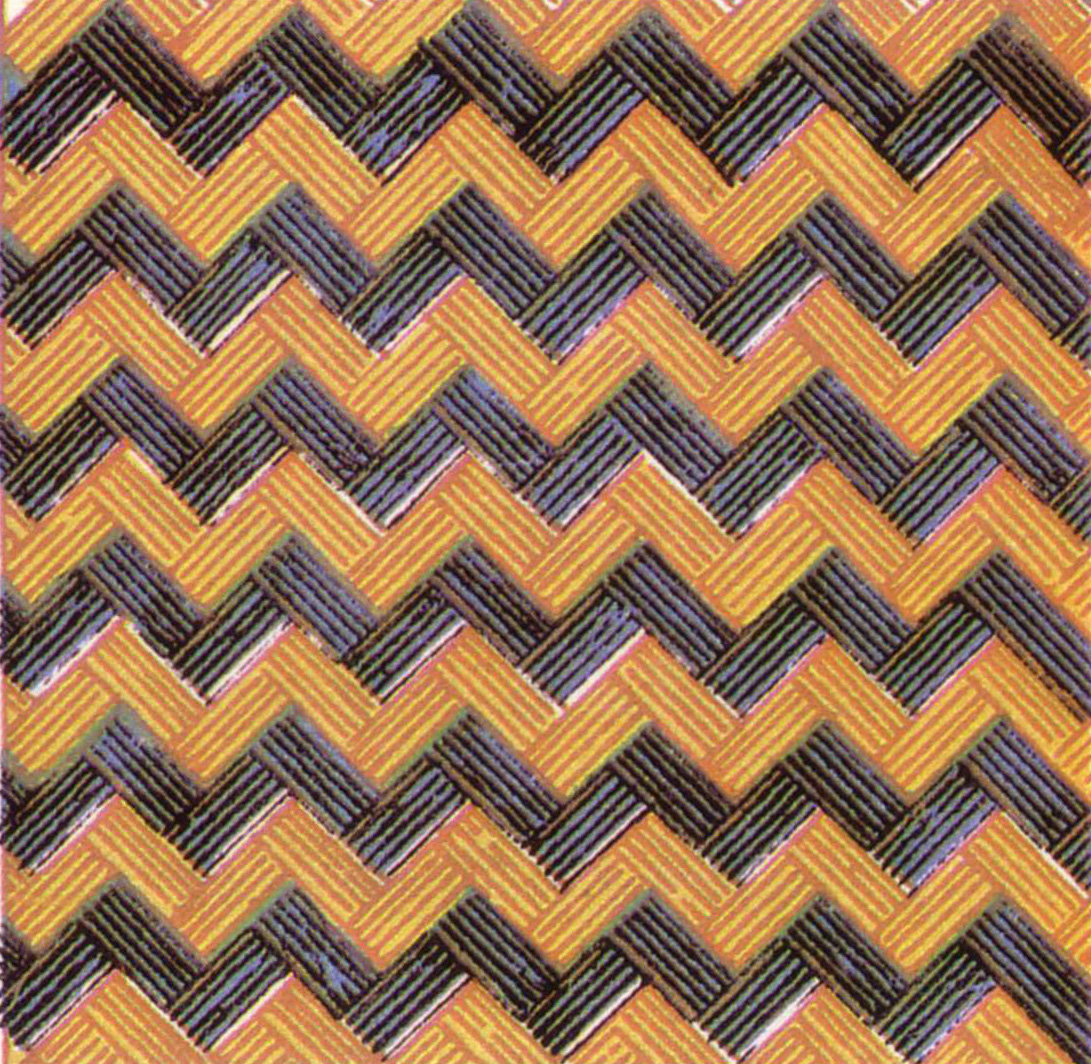
\includegraphics[width=4cm]{Wallpaper_group-pg-1.jpg}
\end{center}
is invariant under a vertical translation and under a horizontal translation with a flip (taking an upward pointing corner to a downward pointing one).
The quotient by those two symmetries is thus the Klein bottle.
\end{example}
\begin{example}
The fundamental group of the real projective space \(\RP{n}\) is \(\Z{}/2\Z{}\) (if \(n\ge 2\)), as we have seen, which clearly has the presentation
\[
\fundamentalGroup{\RP{n}} = \left<x|x^2=1\right>.
\]
\end{example}

\section{Amalgamations}
Suppose that \(G\) and \(H\) are two groups.
We would like to define a group \(G*H\), which contains \(G\) and \(H\), and is otherwise ``as unconstrained as possible''.
The product \(G \times H\) is not ``unconstrained'', because the elements of \(G\) commute with those of \(H\) inside \(G \times H\).

First, note that any group \(G\) has an obvious group morphism \(\left<G\right> \to G\) given by \(g \mapsto g\).
It will help to write out concatenations using some symbol like
\[
g_1 * g_2 * \dots * g_n \in \left<G\right>.
\]
Then we can write our group morphism as
\[
g_1 * g_2 * \dots * g_n \in \left<G\right> \mapsto g_1 g_2 \dots g_n \in G.
\]
This group morphism is clearly surjective, with kernel precisely the group \(N_G \subset \left<G\right>\) whose elements are the concatenations
\[
g_1 * g_2 * \dots * g_n
\]
for which \(g_1 g_2 \dots g_n=1\).
So we can write
\[
G=\left<G|N_G\right>.
\]
Think of \(N_G\) as encoding all of the equations satisfied inside the group \(G\).

We define the \emph{free product}\define{free!product} \(G*H\)\Notation{G*H}{G*H}{amalgation} to be the group \(\left<G \sqcup H|N_G \sqcup N_H\right>\) generated by the elements of \(G\) and \(H\), subject to the relations consisting of all equations satisfied by elements of \(G\) together with all equations satisfied by elements of \(H\).

Another way to look at this: a \emph{word}\define{word} in \(G,H\) is a finite sequence of elements of \(G\) and of \(H\) (perhaps empty), written beside one another with \(*\) symbols inbetween, like
\[
g_1 * g_2 * h_1 * g_3 * h_2 * h_3 * g_4,
\]
et cetera.
We denote the empty sequence as \(1\).
We \emph{reduce} a word by deleting any appearance of the identity element (of either group), and also by replacing any two neighboring elements from the same group by their product in that group:
\[
g_1 * g_2 \mapsto g_1 g_2.
\]
A word is \emph{reduced}\define{word!reduced}\define{reduced word} if we cannot further reduce it.
The group \(G*H\) is the set of reduced words, with multiplication being simply writing down one word after another and then reducing.

A further wrinkle: suppose that \(K \subset G\) is a subgroup which also appears as a subgroup of \(H\): \(K \subset H\).
The \emph{amalgamation}\define{amalgamation} of \(G\) and \(H\) over \(K\), denoted \(G*_K H\),\Notation{G*KH}{G*_K H}{amalgation over a subgroup} is
\[
G *_K H = \left<G \sqcup H|N_G \sqcup N_H \sqcup E\right>
\]
where \(E\) is the collection of equations \(k_G=k_H\) where \(k_G\) is an element of \(K\) as a subgroup of \(G\), and \(k_H\) is the associated element of \(K \subset H\).
Equivalently, we can think of allowing reduced words to be acted on by inserting into any reduced word an element of \(K\) right of an element of \(G\), and left of the next element of \(H\), and vice versa.
There is no longer any straightforward description in terms of reduced words, but the trivial elements, once reduced, are products \(k_1 * k_1^{-1} * \dots * k_n * k_n^{-1}\).

Similarly, if we have a collection of groups \(G_a\), for \(a\) in some set, the \emph{free product} \(*G_a\) is the quotient 
\[
\left<\bigsqcup_a G_a|\bigsqcup_a N_{G_a}\right>,
\]
and if we have some groups \(K_c\) and various morphisms \(\phi_{ca} \colon K_c \to G_a\), the \emph{amalgamation} \(*_{K_c} G_a\) is
\[
\left<\bigsqcup_a G_a|\bigsqcup_a N_{G_a}\sqcup E\right>,
\]
where \(E\) is the set of all equations \(\phi_{ca}(k)=\phi_{cb}(k)\) where \(k \in K_c\).

\section{van~Kampen's theorem II}
\begin{theorem}[van~Kampen II]\label{theorem:van.Kampen.II}\define{van~Kampen's theorem}\define{theorem!van~Kampen}
Take a path connected and locally simply connected topological space \(X\), and a cover by path connected open sets \(X_a \subset X\), with path connected intersections \(X_{ab} \defeq X_a \cap X_b\), all containing some point \(x_0 \in X\).
Let \(\pi\defeq\fundamentalGroup{X,x_0}\), \(\pi_a\defeq\fundamentalGroup{X_a,x_0}\), and so on, with obvious commutative diagrams
\[
\begin{tikzcd}
\pi_{ab} \arrow{r}{} \arrow{d}{} & \pi_a \arrow{d}{} \\
\pi_b \arrow{r}{}
& \pi \\
\end{tikzcd}
\]
Then
\(
\pi=*_{\pi_{bc}} \pi_a
\)
is the amalgamation of all \(\pi_a\) over all \(\pi_{ab}\).
\end{theorem}
\begin{proof}
Let \(\Gamma\defeq *_{\pi_{bc}} \pi_a\).
There are obvious morphisms of groups
\[
\begin{tikzcd}
\pi_{ab} \arrow{r}{} \arrow{d}{} & \pi_a \arrow{d}{} \arrow[bend left]{rdd} \\
\pi_b \arrow{r}{} \arrow[bend right]{rrd}
& \pi \\
& & \Gamma
\end{tikzcd}
\]
given by taking each word in \(\pi_a\) as giving a word in the larger alphabet of \(\Gamma\).
By theorem~\vref{theorem:van.Kampen.I}, there is a unique group morphism \(\pi \to \Gamma\) make commutative all diagrams
\[
\begin{tikzcd}
\pi_{ab} \arrow{r}{} \arrow{d}{} & \pi_a \arrow{d}{} \arrow[bend left]{rdd} \\
\pi_b \arrow{r}{} \arrow[bend right]{rrd}
& \pi \arrow{rd}{} \\
& & \Gamma 
\end{tikzcd}
\]
This morphism of groups is surjective, because it includes the image of every \(\pi_a\).

The group morphisms \(\pi_a \to \pi\) determine a single group morphism \(*\pi_a \to \pi\) of the free product.
Take any loop in \(X\); lemma~\vref{lemma:pick.times} splits it into intervals, say \(x_i(t)\defeq\left.x\right|_{[t_i,t_{i+1}]}\),  remaining each in a single \(X_{a_i}\).
Adding a little on at the beginning and end of those intervals, because every \(X_a\) is path connected and contains \(x_0\), we can arrange that \(x_i(t)\) is a loop starting and ending at \(x_0\).
Hence \(*\pi_a \to \pi\) is surjective.

The kernel of the composition \(* \pi_a \to \pi \to \Gamma\) is precisely the subgroup generated by the various words 
\(k_a * k_b^{-1}\) where \(k_a\) and \(k_b\) are the images in \(\pi_a\) and \(\pi_b\) of some \(k \in \pi_{ab}\).
The element \(k\) is a loop \([x]\) in \(X_{ab}\), and so becomes that loop sitting in either \(X_a\) and \(X_b\), and both of those become the same loop in \(X\), so this word becomes trivial in \(\pi\).
So \(\pi \to \Gamma\) is injective.
\end{proof}
\begin{example}
Suppose that \(X\) is the sphere of dimension \(n \ge 2\).
Let \(X_1\) and \(X_2\) be the sphere punctured at the south pole and the north pole.
So \(X_{12}\) is the sphere with two punctures.
These are all path connected, and \(\set{1}=\pi_1=\pi_2\), so \(\set{1}=\pi\): \(X\) is simply connected.
\end{example}
\begin{example}
Suppose that \(X\) is the bouquet of \(n\) circles, say joined at a point \(x_0 \in X\).
We define each \(X_1,\dots,X_n\) to be \(X\) with all but one of the circles punctured, and hence homotopy equivalent to a single circle.
So \(\pi_i=\fundamentalGroup{X_i,x_0}=\Z{}\).
The various \(\pi_{ij}\) are all trivial: all circles are punctured.
So \(\pi=\Z{} * \dots * \Z{}=*^n \Z{}\).
\end{example}
\begin{example}
If \(Y_a\) are path connected and locally simply connected spaces with marked points \(x_a \in Y_a\), and let \(Y=*Y_a\) be the join of them along those points, then we can take simply connected neighborhoods \(U_a \subset Y_a\) of \(x_a\), and let \(X_a\) be the join \(Y_a* *_{b\ne a} U_b\).
Then \(\pi_{ab} = \set{1}\) and so \(\pi=*\pi_a\), i.e. the fundamental group of the join at points is the free product of the fundamental groups.
\end{example}
\begin{example}
Puncture a torus, and gently widen the puncture, until you see a pair of ``belts'' attached; homotopy equivalent to a bouquet of two circles.
A torus, say with fundamental group \(\left<x,y|xy=yx\right>\), becomes punctured, and becomes a bouquet of circles with fundamental group \(\left<x,y\right>\), included into the torus as \(x,y\mapsto x,y\).
\end{example}
\begin{example}
Suppose that \(X\) is a connected manifold of dimension at least 3; pick a point \(p_0 \in X\).
Take a chart around \(p_0\), with connected domain, and a point \(x_0 \in X\) in the domain of the chart.
Let \(X_2\) be an open set identified by the chart with the interior of a closed ball.
Cover \(X\) in the open set \(X_1=X-\set{p_0}\) and \(X_2\).
They intersect in the set \(X_0=X_1\cap X_2\), homeomorphic to a punctured ball according to the chart.
Then \(\pi_2=\set{1}\) and \(\pi_0=\set{1}\), so \(\pi=\pi_1\), i.e. \(\fundamentalGroup{M-\set{p_0},x_0}=\fundamentalGroup{M,x_0}\): deleting a point does not affect the fundamental group of a manifold of dimension 3 or more.
\end{example}
\begin{example}
How does poking a hole affect the fundamental group of a surface?
Suppose that \(X\) is a connected surface; pick a point \(p_0 \in X\).
Take a \emph{chart} around \(p_0\): a homeomorphism from a connected neighborhood of \(p_0\) to an open subset of the plane.
Take a point \(x_0 \in X\) in the domain of the chart.
Let \(X_2\) be an open set identified by the chart with the interior of a closed disk in the plane.
Cover \(X\) in the open set \(X_1=X-\set{p_0}\) and \(X_2\).
They intersect in the set \(X_0=X_1\cap X_2\), homeomorphic to a punctured ball according to the chart.
Then \(\pi_2=\set{1}\) and \(\pi_0=\Z{}\).
so \(\pi=\pi_1*_{\Z{}} 1=\pi_1/N\), where \(N\) is the normal subgroup generated by the puncture.
\end{example}
\documentclass[tikz]{standalone}
\usepackage{graphicx}
\usepackage{tikz}
\begin{document}
\begin{tikzpicture}
%\fill[blue!20] (-1.6cm,-1.8cm) rectangle (9.5cm,1.8cm);
\node at (0,0) {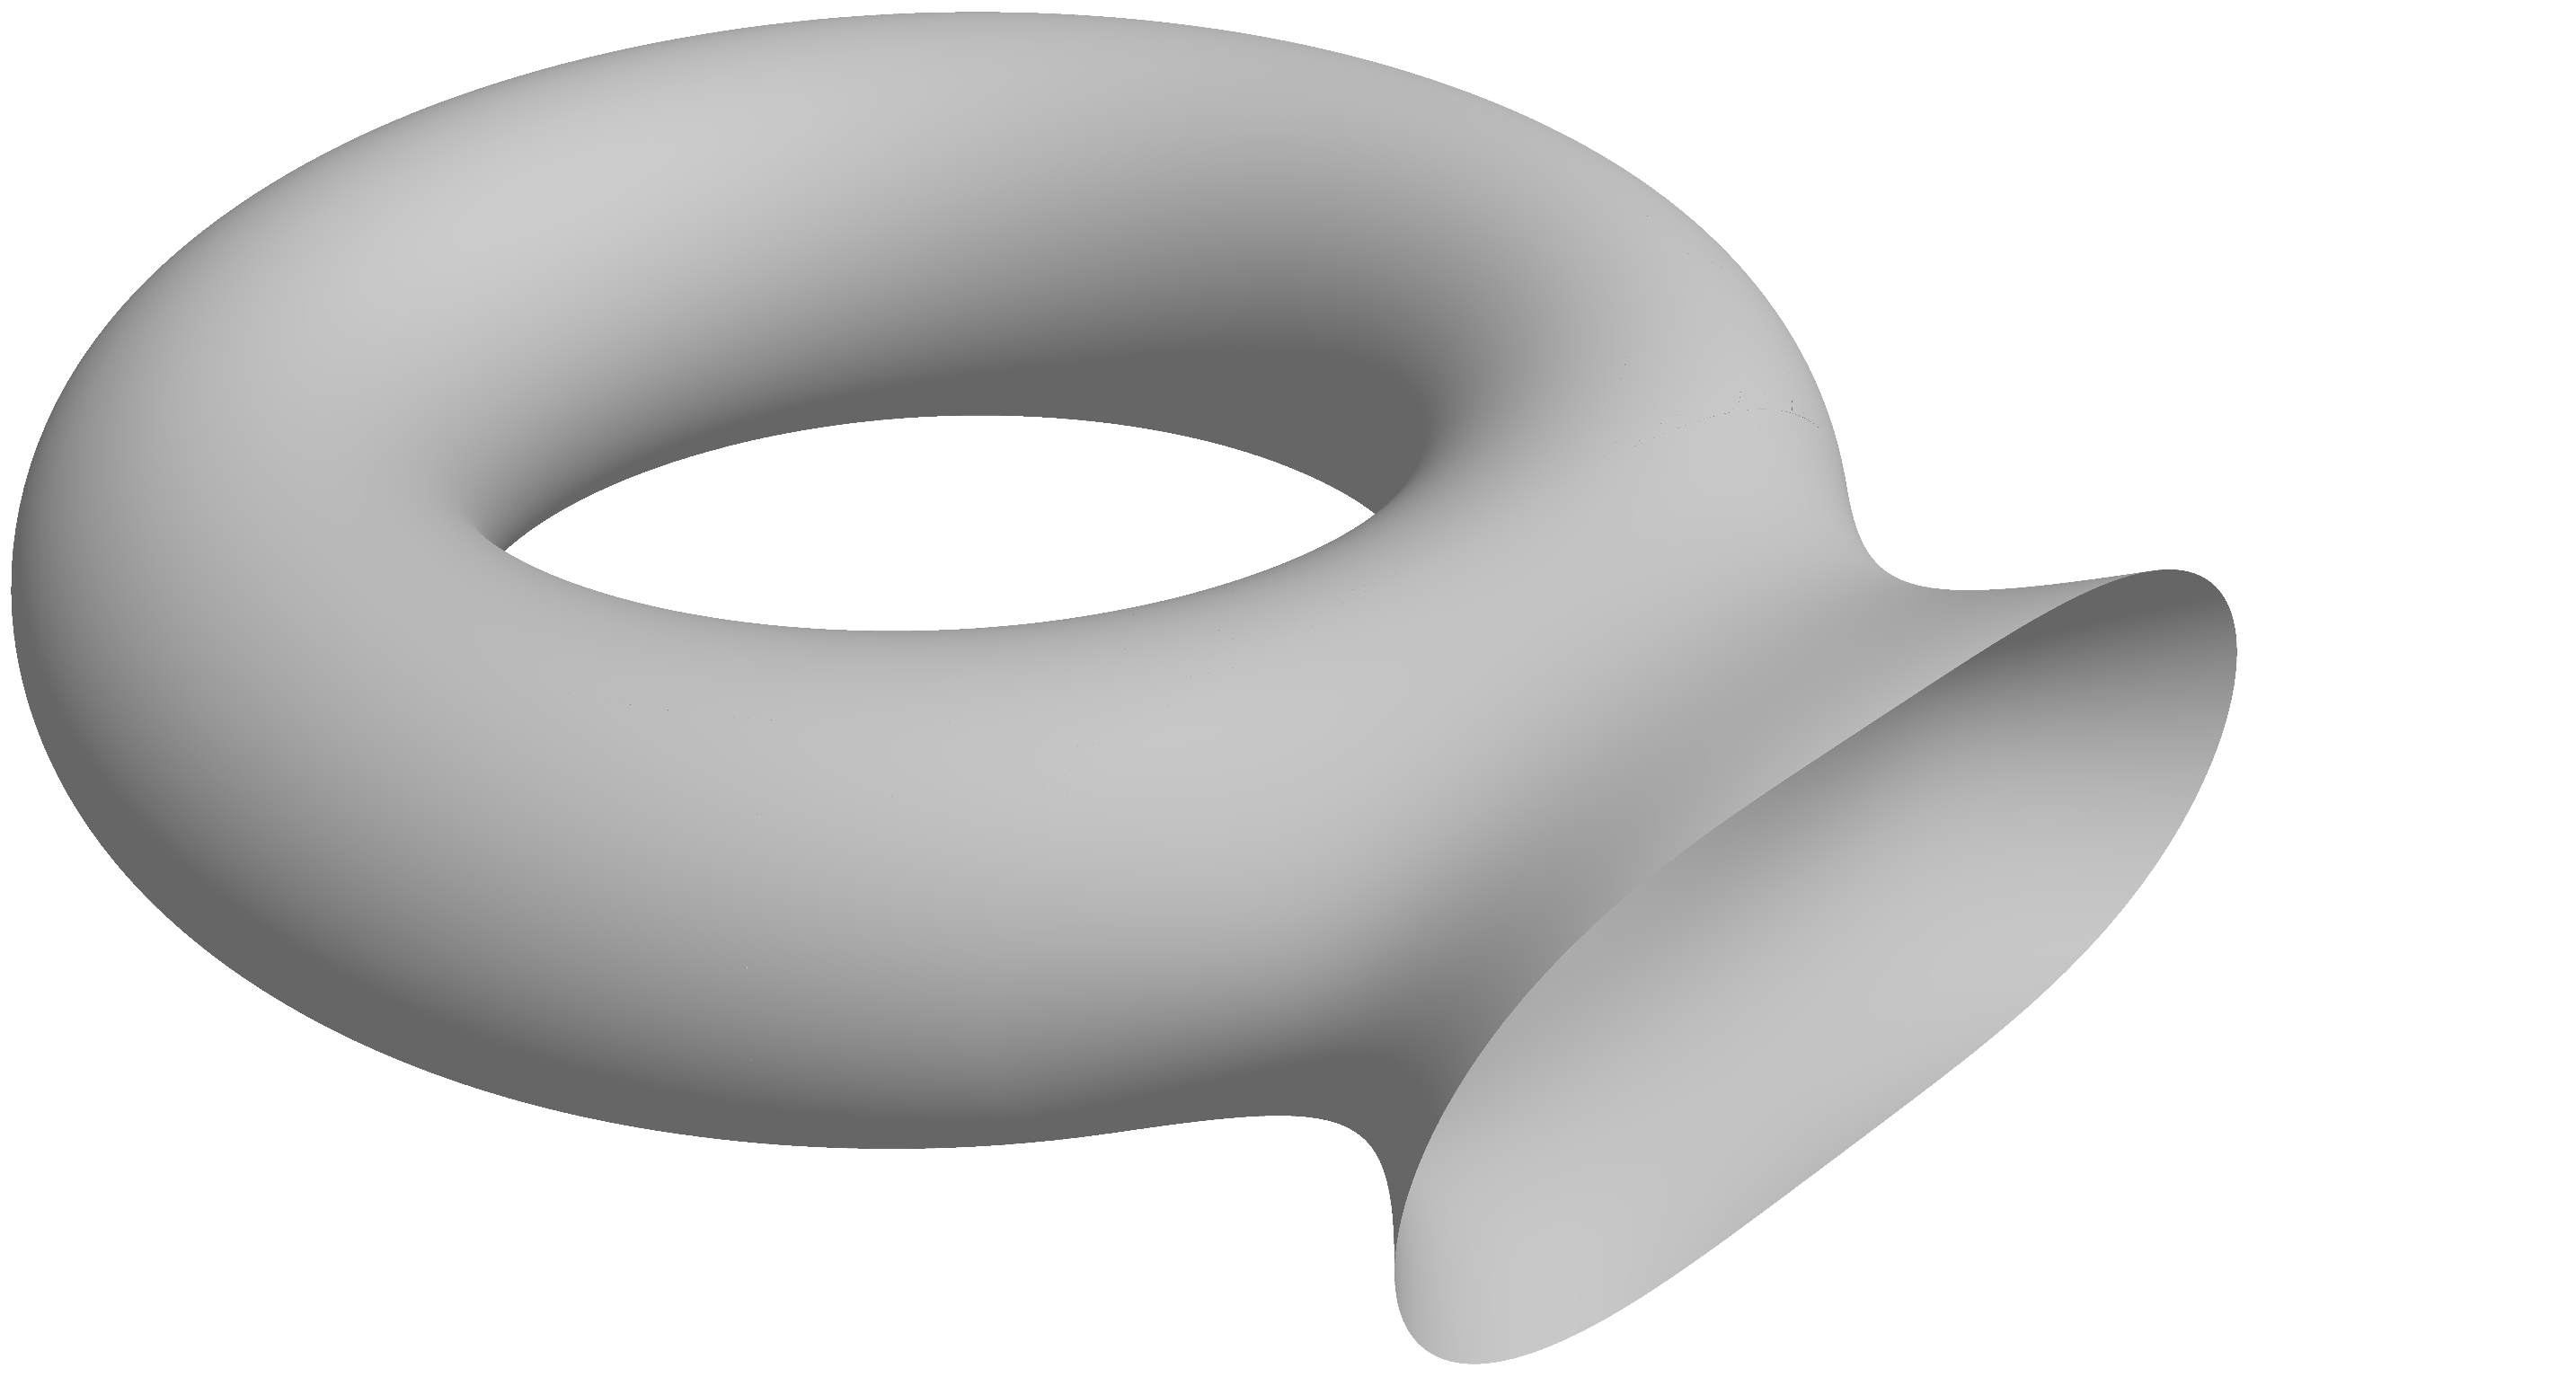
\includegraphics[width=3cm]{torus-with-hole}};
\node at (2.6cm,0) {\reflectbox{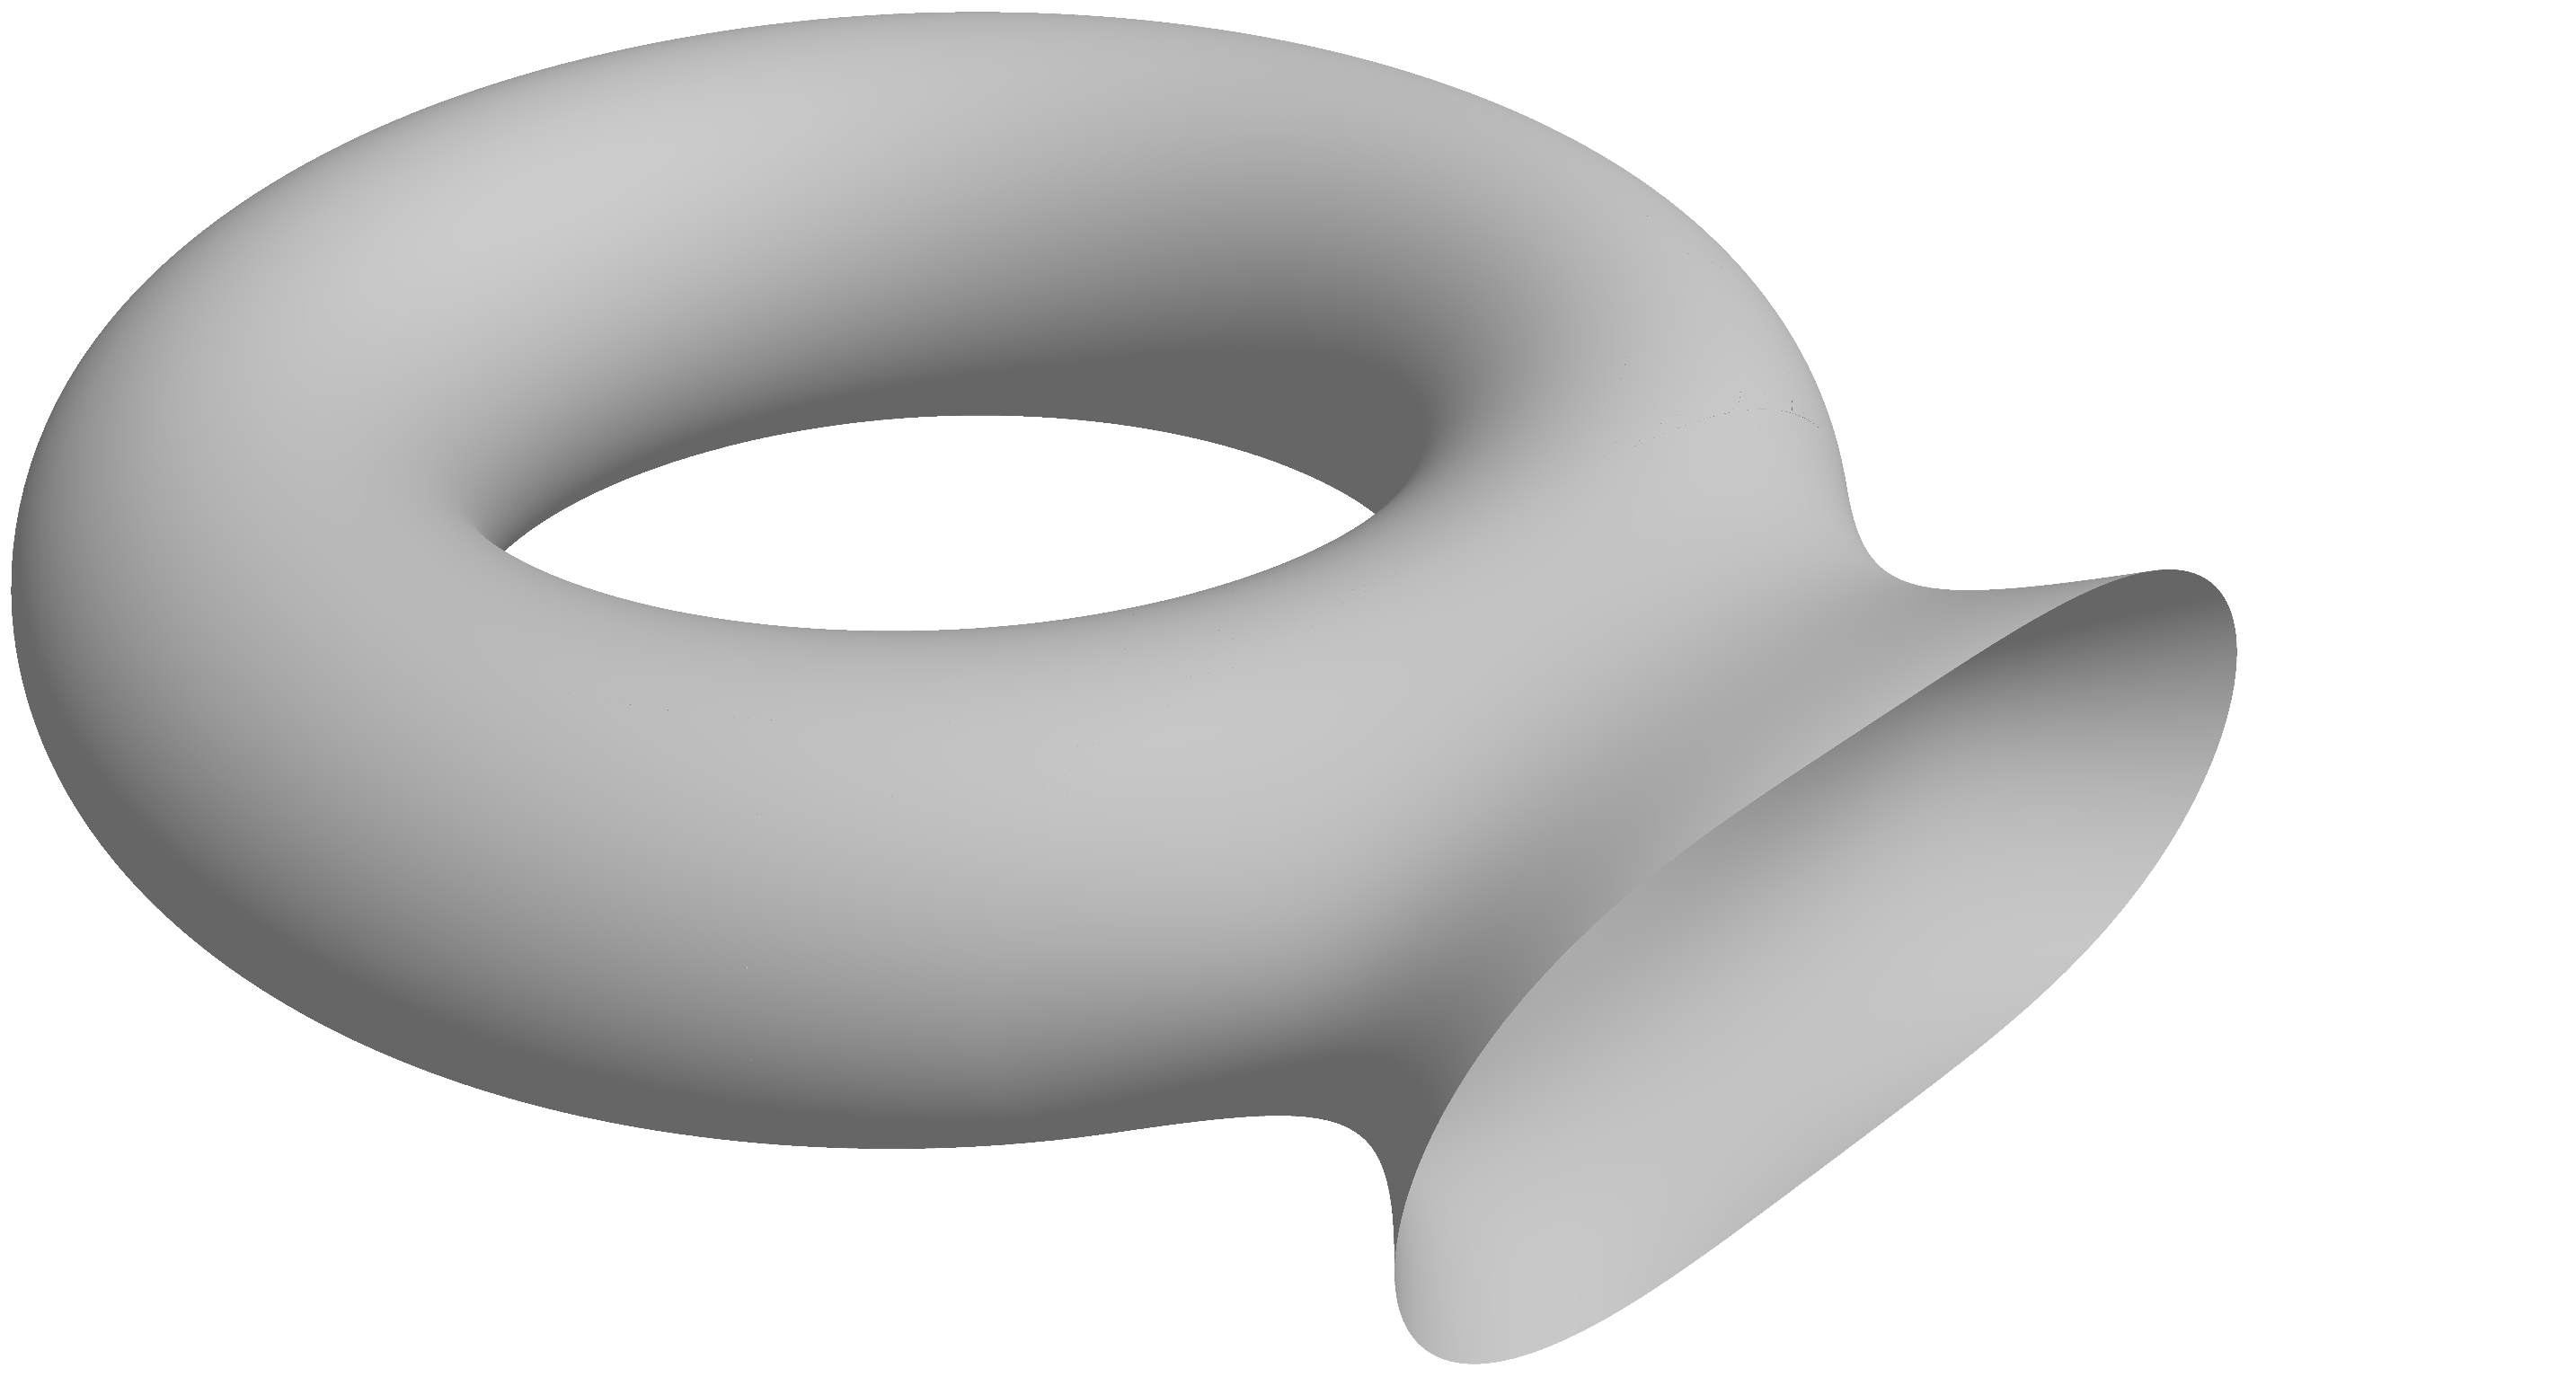
\includegraphics[width=3cm]{torus-with-hole}}};
\node at (1.3cm,0) {\(+\)};
\node at (4.27cm,0) {\(=\)};
\node at (6.84cm,0) {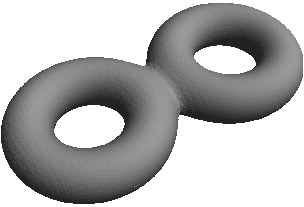
\includegraphics[width=5cm]{genus-2-surface}};
\end{tikzpicture}
\end{document}

\begin{example}
Take two tori, poke holes in them, and join together along a tube; let \(X\) be the resulting surface of genus \(2\).
Each punctured torus is an open set \(X_1, X_2 \subset X\), and the tube is their intersection \(X_0=X_1 \cap X_2\).
The tube \(X_0\) has fundamental group \(\pi_0=\Z{}\), and this includes into each fundamental group of each punctured torus as a small circle around the puncture.
On each torus, the circle around the puncture is the product \(xyx^{-1}y^{-1}\), which of course vanishes once we close up the puncture.
So if we glue two tori together, the resulting surface \(X\) of genus \(2\) has fundamental group 
\[
\left<x,y,X,Y|xyx^{-1}y^{-1}=XYX^{-1}Y^{-1}\right>.
\]
\end{example}
\begin{problem}{covering.spaces:compact.fg}
Prove that the fundamental group of any compact, path connected, and locally simply connected topological space is finitely presented.
\end{problem}


\section{Homotopy groups}
For any topological space \(X\) with marked point \(x_0\), and any \(n\ge 1\), let \(\homotopyGroup{n}{X,x_0}\) be the set of all continuous maps \([0,1]^n \to X\) taking every boundary point of \([0,1]^n\) to \(x_0\), modulo homotopy through such maps.
Each \(\homotopyGroup{n}{X,x_0}\) has a distinguished point: the constant map.

There is a special case: \(n=0\).
We define \(\homotopyGroup{0}{X,x_0}\) to be the set of all components of \(X\), with a special chosen component: that of \(x_0\).
Make \(\homotopyGroup{0}{X,x_0}\) into a topological space, by the quotient topology.

For \(n\ge 1\), take \(f,g \colon [0,1]^n \to X\) each mapping the boundary of \([0,1]^n\) to \(x_0\).
Define \(f*g\) to be the usual 
\[
(f*g)(t,x_2,\dots,x_n) =
\begin{cases}
f(2t,x_2,\dots,x_n), & \text{if \(0 \le t\le \frac{1}{2}\)}, \\
g(2t-1,x_2,\dots,x_n), & \text{if \(\frac{1}{2} \le t\le 1\)},
\end{cases}
\]
and \(\bar{f}(t,x_2,\dots,x_n)=f(1-t,x_2,\dots,x_n)\).
If \(f \colon X \to Y\) is continuous, and \(y_0\defeq f(x_0)\), define \(f_* \colon \homotopyGroup{*}{X,x_0} \to \homotopyGroup{*}{Y,y_0}\) by \(f_*[g] = [f \circ g]\).

A \emph{contraction}\define{contraction} of a topological space \(X\) to a point \(x_0\in X\) is a continuous map \(\varphi\colon X\times[0,1]\to X\) so that \(\varphi(x,0)=x\) and \(\varphi(x,1)=x_0\) for any \(x\in X\).
A topological space \(X\) is \emph{contractible}\define{contractible} if it has a contraction.
\begin{problem}{covering.space:contractible}
Prove that every contractible space is connected and has trivial homotopy groups.
\end{problem}
Given a continuous map \(f \colon X \to Y\), a \emph{lift}\define{lift} of a continuous map \(g \colon Z \to Y\) is a continuous map \(\hat{g} \colon Z \to X\) so that \(f \circ \hat{g}=g\).
A \emph{Serre fibration}\define{Serre fibration} is a continuous map \(f \colon X \to Y\) of topological spaces, so that for any box \(Z=[0,1]^n\) and continuous map \(g \colon Z \times [0,1] \to Y\), denoted \(g_t(z)\defeq g(z,t)\), every lift of \(g_0\) extends to a lift of \(g\).
\begin{theorem}
If \(f \colon X \to Y\) is a Serre fibration, then the obvious maps 
\[
\homotopyGroup{n}{F,x_0}\to\homotopyGroup{n}{X,x_0}\to\homotopyGroup{n}{Y,y_0}
\]
fit together into an exact sequence
\begingroup
\newcommand*{\xA}[1]{\homotopyGroup{#1}{F,x_0}}
\newcommand*{\xB}[1]{\homotopyGroup{#1}{X,x_0}}
\newcommand*{\xC}[1]{\homotopyGroup{#1}{Y,y_0}}
\reverseLongExactSequence{\xA}{\xB}{\xC}
\endgroup
\end{theorem}

Pick \(x_0 \in X\), let \(y_0\defeq f(x_0)\) and let \(F\defeq f^{-1}\set{y_0}\subseteq X\).
The morphism \(\fundamentalGroup{X,x_0}\to\fundamentalGroup{Y,y_0}\) kills loops in \(X\) which lie entirely in a fiber \(F=f^{-1}\set{y_0}\), i.e. those loops map to \(1\in\fundamentalGroup{Y,y_0}\).
More generally, it kills the loops in \(X\) which admit a homotopy, fixing endpoints, to a loop in \(F\).
Any loop in \(Y\) starting and ending at \(y_0\) lifts to a path in \(X\), starting at \(x_0\), but perhaps not a loop.
Since it is a loop in \(Y\), its lift has ends in \(X\) lying in the fiber \(F\).
Under homotopy of the loop in \(Y\), with fixed ends, the ends of the lift can only move inside \(F\), so they have well defined components, a map 
\[
\fundamentalGroup{X,x_0}\to\fundamentalGroup{Y,y_0}\to\homotopyGroup{0}{F,x_0},
\]
where \(\homotopyGroup{0}{X_{y_0},x_0}\) is the set of all path components of \(X_{y_0}\), and contains a distinguished element, the path component that contains \(x_0 \in X_{y_0}\).
If the ends of that lift lie in the same path component, then we can draw those two ends together, obtaining the path in \(Y\) from a path in \(X\), i.e. the image of the first map is the ``kernel'' of the second, i.e. the elements mapping to the distinguished component.

Take a continuous map \(h \colon Z \times [0,1] \to Y\), which we write as \(h_t(z)=h(z,t)\).
Suppose that \(h_0(z)=y_0\) for all \(z\), and \(h_s(z)=y_0\) for all \(z\in\partial Z\).
Lift \(h_0\) to the trivial map to \(x_0\).
Lift \(h\) to a map \(\hat{h} \colon Z \times [0,1] \to X\) extending that lift.
So \(f \circ \hat{h}_t(z)=h_t(z)\), and \(\hat{h}_0(z)=x_0\) for all \(z \in Z\).
Since \(h_s(z)=y_0\) for \(z \in \partial Z\), \(\hat{h}_s(z) \in F\) for \(z\in\partial Z\), for all \(s\).
In particular, \(\hat{h}_s(z)\) stays in the component of \(x_0\) in \(F\), for \(z\in\partial Z\), for all \(s\).
If we replace our choices at each step, still \(\hat{h}_1 \colon \partial Z \to F\) varies only by homotopy, giving an element of \(\homotopyGroup{n-1}{F,x_0}\), a map
\[
\homotopyGroup{n}{X,x_0}\to\homotopyGroup{n}{Y,y_0}\to\homotopyGroup{n-1}{F,x_0}.
\]
If this element vanishes, then \(\hat{h}_1\) is nulhomotopic in \(F\), and if we attach that homotopy to \(\hat{h}\), and its composition with \(X\to Y\) to \(h\), then \(h\) continues to map to \(h_s(z)=y_0\).
So \(h\) is an element of \(\homotopyGroup{n}{Y,y_0}\) arising from an element of \(\homotopyGroup{n}{X,x_0}\).
In other words, in
\[
\homotopyGroup{n}{X,x_0}\to\homotopyGroup{n}{Y,y_0}\to\homotopyGroup{n-1}{F,x_0}.
\]
 the kernel of the second map is the image of the first.

Being a Serre fibration is a local property in \(Y\):
\begin{lemma}\label{lemma:Serre.fibration.local}
A continuous map \(f \colon X \to Y\) of topological spaces is a Serre fibration if and only if there is an open cover of \(Y\) by open sets \(Y_a \subseteq Y\) so that, if \(X_a\defeq f^{-1}Y_a\) and \(f_a \defeq \left.f\right|_{X_a}\), then each \(f_a\) is a Serre fibration.
\end{lemma}
\begin{proof}
Take such an open cover, and some map \(g \colon Z \times [0,1] \to Y\) with a lift \(\hat{g}_0 \colon Z \to X\), where \(Z=[0,1]^n\).
Cover the image of \(g\) in our open sets \(Y_a\).
Take a finite subcover.
Divide up \(Z\times [0,1]\) into a grid of cubes small enough that each lies inside a single \(Y_a\).
Lift up one cube at a time.
\end{proof}
A \emph{projection}\define{projection map} is a map \((x,z)\in X \times Z\mapsto z \in Z\); the \emph{fiber} is \(Z\).
Two maps \(X_0 \to Y_0\) and \(X_1\to Y_1\) are \emph{isomorphic} if there are diffeomorphisms \(X_0 \to X_1\) and \(Y_0\to Y_1\)  making a commutative diagram
\begin{tikzcd}
X_0 \arrow{r} \arrow{d} & X_1 \arrow{d} \\
Y_0 \arrow{r} & Y_1
\end{tikzcd}
A continuous map is \emph{trivial} if isomorphic to a projection.
A continuous map \(\pi\colon X \to Y\) is \emph{locally trivial} ifevery point of \(Y\) lies in an open set \(U\subseteq Y\)  so that 
\[
\left.\pi\right|_{\pi^{-1}U}\colon \pi^{-1}U \to U
\]
is trivial.
A \emph{fiber bundle}\define{fiber bundle} is a continuous locally trivial map \(\pi\colon X \to Y\) of topological spaces.
\begin{lemma}
Every fiber bundle is a Serre fibration.
\end{lemma}
\begin{proof}
Fiber bundles are locally trivial, so true locally; apply lemma~\vref{lemma:Serre.fibration.local}.
\end{proof}

\chapter{The Brouwer fixed point theorem}
\section{The hex game}
A \emph{hex board}\define{hex!board}\define{board!hex} is a diamond of regular hexagonal tiles, with an equal number of hexagons on each side.
\begin{center}
\tiny
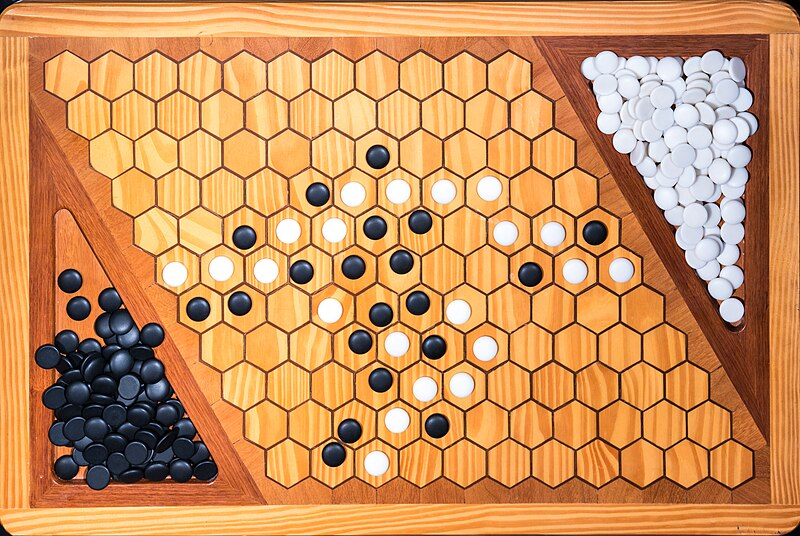
\includegraphics[width=\textwidth]{hex-board}
\par\noindent{}Exhibit made by Massami Takahashi, photo by Rodrigo.Argenton.
Creative Commons Attribution-Share Alike 4.0 International license.
\end{center}
A game of \emph{hex}\define{hex} is played on such a board.
One player has black stones, and aims to connect the left and right edges of the board with a path of her stones on neighboring tiles.
The other has white stones, and similarly aims to connect the top and bottom edges of the board with a path of his stones on neighboring tiles
The four corner hexagons each neighbor both sides, so either player can start or end such a path at a corner.
Before the black player takes the first turn, the board is empty of stones.
The players take turns placing a stone of their color on a single tile on the board, which has not previously received a stone.
The first to achieve their aim wins.
The game ends in a draw if neither wins and every tile contains a stone.
\begin{theorem}\label{theorem:hex.has.a.winner}
Every game of hex has a winner.
\end{theorem}
Before giving the proof, it is more convenient to draw the hex board differently.
Take a square, divided into a grid of squares.
Draw a diagonal line south west to north east through each small square, dividing the small square into two triangles.
Draw a gray disk at each corner of every small square.
\[
\begin{tikzpicture}[scale=.5]
\draw (0,0) grid (6,6);
\foreach \i in {0,...,5}
{
	\foreach \j in {0,...,5}
	{
		\draw (\i,\j) -- ({1+\i},{1+\j});
	}
}
\foreach \i in {0,...,6}
{
	\foreach \j in {0,...,6}
	{
		\draw[black,fill=gray!50] (\i,\j) circle (.25cm);
	}
}
\end{tikzpicture}
\]
The disks are the tiles.
Each tile has neighboring tiles at the corners of any small square it overlaps, and also across those squares on the diagonal lines.
Each interior tile has \(6\) neighbors, each edge tile \(4\) neighbors, the upper right and lower left corner tiles have \(3\) neighbors, and the upper left and lower right corner tiles have \(2\) neighbors.
Henceforth we only make use of this type of hex board; we leave the reader to work out how to turn one type of hex board into the other.
\begin{proof}
Our proof is by contradiction.
Each step leads to one fewer empty tile.
So if neither side wins, we can suppose that they keep playing until every tile on the board contains a stone, and yet somehow there is no path of white stones travelling from the left edge to the right, and no path of black stones from the top to the bottom.
Imagine that every disk, which we draw as gray, actually contains either a black or white stone, so should really be coloured either black or white.

We first add onto each side of the board a new row or column of tiles, of the same size as the board, so forming a square without its corners, with the diagonal lines, south west to north east, added at the two corners where that is possible (the upper left and lower right):
\[
\begin{tikzpicture}[scale=.5]
\draw (-1,0) grid (7,6);
\draw (0,-1) grid (6,7);
\foreach \i in {-1,...,6}
{
	\foreach \j in {0,...,5}
	{
		\draw (\i,\j) -- ({1+\i},{1+\j});
	}
}
\foreach \i in {0,...,6}
{
\draw ({\i-1},6) -- (\i,7);
\draw (\i,-1) -- ({\i+1},0);
}
\foreach \i in {0,...,6}
{
	\foreach \j in {-1,...,7}
	{
		\draw[black,fill=gray!50] (\i,\j) circle (.25cm);
	}
	\draw[black,fill=white] (\i,-1) circle (.25cm);
	\draw[black,fill=white] (\i,7) circle (.25cm);
	\draw[black,fill=black] (-1,\i) circle (.25cm);
	\draw[black,fill=black] (7,\i) circle (.25cm);
}
\end{tikzpicture}
\]
We put black stones in all of the new left and right tiles, and white in all of the new top and bottom tiles.
Don't step on the stones, but only on the triangles; start at the lower right corner triangle:
\[
\begin{tikzpicture}[scale=.5]
\fill[blue!20] (6,-1) -- (7,0) -- (6,0) -- cycle;
\draw (-1,0) grid (7,6);
\draw (0,-1) grid (6,7);
\foreach \i in {-1,...,6}
{
	\foreach \j in {0,...,5}
	{
		\draw (\i,\j) -- ({1+\i},{1+\j});
	}
}
\foreach \i in {0,...,6}
{
\draw ({\i-1},6) -- (\i,7);
\draw (\i,-1) -- ({\i+1},0);
}
\foreach \i in {0,...,6}
{
	\foreach \j in {-1,...,7}
	{
		\draw[black,fill=gray!50] (\i,\j) circle (.25cm);
	}
	\draw[black,fill=white] (\i,-1) circle (.25cm);
	\draw[black,fill=white] (\i,7) circle (.25cm);
	\draw[black,fill=black] (-1,\i) circle (.25cm);
	\draw[black,fill=black] (7,\i) circle (.25cm);
}
\end{tikzpicture}
\]

An edge is \emph{mixed} if it has a white stone on one tile and a black stone on the other.
A triangle is \emph{mixed} if not all of its stones are the same colour, so it has a black stone on one corner and a white stone on another corner.
The third corner then has a black or white stone on it.
So every mixed triangle has two mixed edges and one edge not mixed.

Our first triangle is mixed: it has a white and black stone on the lower right edge.
So it has a second mixed edge.
Step over that edge to the next triangle.

Suppose inductively that we are on a mixed triangle, and we entered it via a mixed edge.
It has precisely one other mixed edge.
We have to step across that edge next.
So there is a uniquely determined sequence of triangles.
We always head across an edge, so we never step on the same triangle two times in a row, since no triangle is a neighbor of itself.

%import random
%for i in range(0,7):
%    for j in range(0,7):
%        n = random.randint(0,1)
%        if (n==0):
%            print("\\draw[black,fill=white] ({0},{1}) circle (.25cm);".format(i,j))
%        else:
%            print("\\draw[black,fill=black] ({0},{1}) circle (.25cm);".format(i,j))        

For example, if we start with:
\[
\begin{tikzpicture}[scale=.5]
\fill[blue!20] (6,-1) -- (7,0) -- (6,0) -- cycle;
\draw (-1,0) grid (7,6);
\draw (0,-1) grid (6,7);
\foreach \i in {-1,...,6}
{
	\foreach \j in {0,...,5}
	{
		\draw (\i,\j) -- ({1+\i},{1+\j});
	}
}
\foreach \i in {0,...,6}
{
\draw ({\i-1},6) -- (\i,7);
\draw (\i,-1) -- ({\i+1},0);
}
\foreach \i in {0,...,6}
{
	\draw[black,fill=white] (\i,-1) circle (.25cm);
	\draw[black,fill=white] (\i,7) circle (.25cm);
	\draw[black,fill=black] (-1,\i) circle (.25cm);
	\draw[black,fill=black] (7,\i) circle (.25cm);
}
\draw[black,fill=black] (0,0) circle (.25cm);
\draw[black,fill=white] (0,1) circle (.25cm);
\draw[black,fill=black] (0,2) circle (.25cm);
\draw[black,fill=white] (0,3) circle (.25cm);
\draw[black,fill=black] (0,4) circle (.25cm);
\draw[black,fill=black] (0,5) circle (.25cm);
\draw[black,fill=black] (0,6) circle (.25cm);
\draw[black,fill=black] (1,0) circle (.25cm);
\draw[black,fill=black] (1,1) circle (.25cm);
\draw[black,fill=black] (1,2) circle (.25cm);
\draw[black,fill=white] (1,3) circle (.25cm);
\draw[black,fill=white] (1,4) circle (.25cm);
\draw[black,fill=white] (1,5) circle (.25cm);
\draw[black,fill=white] (1,6) circle (.25cm);
\draw[black,fill=white] (2,0) circle (.25cm);
\draw[black,fill=white] (2,1) circle (.25cm);
\draw[black,fill=black] (2,2) circle (.25cm);
\draw[black,fill=black] (2,3) circle (.25cm);
\draw[black,fill=white] (2,4) circle (.25cm);
\draw[black,fill=black] (2,5) circle (.25cm);
\draw[black,fill=black] (2,6) circle (.25cm);
\draw[black,fill=white] (3,0) circle (.25cm);
\draw[black,fill=white] (3,1) circle (.25cm);
\draw[black,fill=black] (3,2) circle (.25cm);
\draw[black,fill=white] (3,3) circle (.25cm);
\draw[black,fill=black] (3,4) circle (.25cm);
\draw[black,fill=black] (3,5) circle (.25cm);
\draw[black,fill=white] (3,6) circle (.25cm);
\draw[black,fill=white] (4,0) circle (.25cm);
\draw[black,fill=black] (4,1) circle (.25cm);
\draw[black,fill=white] (4,2) circle (.25cm);
\draw[black,fill=black] (4,3) circle (.25cm);
\draw[black,fill=black] (4,4) circle (.25cm);
\draw[black,fill=black] (4,5) circle (.25cm);
\draw[black,fill=white] (4,6) circle (.25cm);
\draw[black,fill=white] (5,0) circle (.25cm);
\draw[black,fill=black] (5,1) circle (.25cm);
\draw[black,fill=black] (5,2) circle (.25cm);
\draw[black,fill=black] (5,3) circle (.25cm);
\draw[black,fill=white] (5,4) circle (.25cm);
\draw[black,fill=white] (5,5) circle (.25cm);
\draw[black,fill=black] (5,6) circle (.25cm);
\draw[black,fill=white] (6,0) circle (.25cm);
\draw[black,fill=white] (6,1) circle (.25cm);
\draw[black,fill=white] (6,2) circle (.25cm);
\draw[black,fill=black] (6,3) circle (.25cm);
\draw[black,fill=white] (6,4) circle (.25cm);
\draw[black,fill=white] (6,5) circle (.25cm);
\draw[black,fill=white] (6,6) circle (.25cm);
\end{tikzpicture}
\]
then our triangles are:
\[
\begin{tikzpicture}[scale=.5]
\fill[blue!20] (6,-1) -- (7,0) -- (6,0) -- cycle;
\fill[blue!20] (6,0) -- (7,0) -- (7,1) -- cycle;
\fill[blue!20] (6,0) -- (7,1) -- (6,1) -- cycle;
\fill[blue!20] (6,1) -- (7,1) -- (7,2) -- cycle;
\fill[blue!20] (6,1) -- (7,2) -- (6,2) -- cycle;
\fill[blue!20] (6,2) -- (7,2) -- (7,3) -- cycle;
\fill[blue!20] (6,2) -- (7,3) -- (6,3) -- cycle;
\fill[blue!20] (5,2) -- (6,2) -- (6,3) -- cycle;
\fill[blue!20] (5,1) -- (6,2) -- (5,2) -- cycle;
\fill[blue!20] (5,1) -- (6,1) -- (6,2) -- cycle;
\fill[blue!20] (5,0) -- (6,1) -- (5,1) -- cycle;
\fill[blue!20] (4,0) -- (5,0) -- (5,1) -- cycle;
\fill[blue!20] (4,0) -- (5,1) -- (4,1) -- cycle;
\fill[blue!20] (3,0) -- (4,0) -- (4,1) -- cycle;
\fill[blue!20] (3,0) -- (4,1) -- (3,1) -- cycle;
\fill[blue!20] (3,1) -- (4,1) -- (4,2) -- cycle;
\fill[blue!20] (4,1) -- (5,2) -- (4,2) -- cycle;
\fill[blue!20] (4,2) -- (5,2) -- (5,3) -- cycle;
\fill[blue!20] (4,2) -- (5,3) -- (4,3) -- cycle;
\fill[blue!20] (3,2) -- (4,2) -- (4,3) -- cycle;
\fill[blue!20] (3,1) -- (4,2) -- (3,2) -- cycle;
\fill[blue!20] (2,1) -- (3,1) -- (3,2) -- cycle;
\fill[blue!20] (2,1) -- (3,2) -- (2,2) -- cycle;
\fill[blue!20] (1,1) -- (2,1) -- (2,2) -- cycle;
\fill[blue!20] (1,0) -- (2,1) -- (1,1) -- cycle;
\fill[blue!20] (1,0) -- (2,0) -- (2,1) -- cycle;
\fill[blue!20] (1,-1) -- (2,0) -- (1,0) -- cycle;
\fill[blue!20] (0,-1) -- (1,-1) -- (1,0) -- cycle;
\fill[blue!20] (0,-1) -- (1,0) -- (0,0) -- cycle;
\draw (-1,0) grid (7,6);
\draw (0,-1) grid (6,7);
\draw[line width=2pt] (6,-1) -- (6,2) -- (6,1) -- (5,0) -- (3,0) -- (3,1) -- (4,2) -- (3,1) -- (2,1) -- (2,0) -- (1,-1) -- (0,-1);
\draw[line width=2pt] (7,0) -- (7,3) -- (6,3) -- (5,2) -- (5,1) -- (4,1) -- (5,2) -- (5,3) -- (4,3) -- (3,2) -- (2,2) -- (1,1) -- (1,0) -- (0,0);
\foreach \i in {-1,...,6}
{
	\foreach \j in {0,...,5}
	{
		\draw (\i,\j) -- ({1+\i},{1+\j});
	}
}
\foreach \i in {0,...,6}
{
\draw ({\i-1},6) -- (\i,7);
\draw (\i,-1) -- ({\i+1},0);
}
\foreach \i in {0,...,6}
{
	\foreach \j in {-1,...,7}
	{
		\draw[black,fill=gray!50] (\i,\j) circle (.25cm);
	}
	\draw[black,fill=white] (\i,-1) circle (.25cm);
	\draw[black,fill=white] (\i,7) circle (.25cm);
	\draw[black,fill=black] (-1,\i) circle (.25cm);
	\draw[black,fill=black] (7,\i) circle (.25cm);
}
\draw[black,fill=black] (0,0) circle (.25cm);
\draw[black,fill=white] (0,1) circle (.25cm);
\draw[black,fill=black] (0,2) circle (.25cm);
\draw[black,fill=white] (0,3) circle (.25cm);
\draw[black,fill=black] (0,4) circle (.25cm);
\draw[black,fill=black] (0,5) circle (.25cm);
\draw[black,fill=black] (0,6) circle (.25cm);
\draw[black,fill=black] (1,0) circle (.25cm);
\draw[black,fill=black] (1,1) circle (.25cm);
\draw[black,fill=black] (1,2) circle (.25cm);
\draw[black,fill=white] (1,3) circle (.25cm);
\draw[black,fill=white] (1,4) circle (.25cm);
\draw[black,fill=white] (1,5) circle (.25cm);
\draw[black,fill=white] (1,6) circle (.25cm);
\draw[black,fill=white] (2,0) circle (.25cm);
\draw[black,fill=white] (2,1) circle (.25cm);
\draw[black,fill=black] (2,2) circle (.25cm);
\draw[black,fill=black] (2,3) circle (.25cm);
\draw[black,fill=white] (2,4) circle (.25cm);
\draw[black,fill=black] (2,5) circle (.25cm);
\draw[black,fill=black] (2,6) circle (.25cm);
\draw[black,fill=white] (3,0) circle (.25cm);
\draw[black,fill=white] (3,1) circle (.25cm);
\draw[black,fill=black] (3,2) circle (.25cm);
\draw[black,fill=white] (3,3) circle (.25cm);
\draw[black,fill=black] (3,4) circle (.25cm);
\draw[black,fill=black] (3,5) circle (.25cm);
\draw[black,fill=white] (3,6) circle (.25cm);
\draw[black,fill=white] (4,0) circle (.25cm);
\draw[black,fill=black] (4,1) circle (.25cm);
\draw[black,fill=white] (4,2) circle (.25cm);
\draw[black,fill=black] (4,3) circle (.25cm);
\draw[black,fill=black] (4,4) circle (.25cm);
\draw[black,fill=black] (4,5) circle (.25cm);
\draw[black,fill=white] (4,6) circle (.25cm);
\draw[black,fill=white] (5,0) circle (.25cm);
\draw[black,fill=black] (5,1) circle (.25cm);
\draw[black,fill=black] (5,2) circle (.25cm);
\draw[black,fill=black] (5,3) circle (.25cm);
\draw[black,fill=white] (5,4) circle (.25cm);
\draw[black,fill=white] (5,5) circle (.25cm);
\draw[black,fill=black] (5,6) circle (.25cm);
\draw[black,fill=white] (6,0) circle (.25cm);
\draw[black,fill=white] (6,1) circle (.25cm);
\draw[black,fill=white] (6,2) circle (.25cm);
\draw[black,fill=black] (6,3) circle (.25cm);
\draw[black,fill=white] (6,4) circle (.25cm);
\draw[black,fill=white] (6,5) circle (.25cm);
\draw[black,fill=white] (6,6) circle (.25cm);
\end{tikzpicture}
\]
We see that we start at one corner and end at another.
The stones on our right hand side are black, and on our left hand side are right.

We want to see that we never step on triangle twice.
Suppose that this sequence of triangles enters a loop sometime after the first step.
Let \(B\) be the first triangle we encounter for a second time.
The first time we reach \(B\), we come from some triangle \(A\), and leave to some triangle \(C\), so our path is \(\dots ABC\dots\).
The second time we reach \(B\), we come across one mixed edge and then leave across another.
But triangles \(A\) and \(C\) are across those edges.
So we must travel \(\dots ABC\dots ABC\dots\) or \(\dots ABC\dots CBA\dots\).
In the first case, \(B\) is not the first triangle we hit twice: we already hit \(A\) twice previously.
In the second case, \(B\) is not the first triangle we hit twice: we already hit \(C\) twice previously.

So if there is a loop, the first repetition is at the first triangle, where we entered:
\[
AB\dots A\dots 
\]
But there is only one mixed edge of \(A\) we can cross through, and we step across it when we reach \(B\).
We must therefore pass across that same edge when we get back to \(A\) again:
\[
AB\dots BA\dots 
\]
Again a contradiction: \(A\) is not the first triangle we reach for a second time.

Since there is no loop in our path of triangles, our path ends.
But we can keep stepping until we reach a triangle whose mixed edge doesn't lead to another triangle.
These can only be triangles at the corners (and even some of them might not be mixed edges): 
\[
\begin{tikzpicture}[scale=.5]
\fill[blue!20] (6,-1) -- (7,0) -- (6,0) -- cycle;
\draw[line width=2pt] (6,-1) -- (7,0);
\fill[blue!20] (-1,6) -- (0,7) -- (0,6) -- cycle;
\draw[line width=2pt] (-1,6) -- (0,7);
\fill[blue!20] (0,-1) -- (1,0) -- (0,0) -- cycle;
\draw[line width=2pt] (0,-1) -- (0,0);
\fill[blue!20] (-1,0) -- (0,1) -- (0,0) -- cycle;
\draw[line width=2pt] (-1,0) -- (0,0);
\fill[blue!20] (6,6) -- (6,7) -- (5,6) -- cycle;
\draw[line width=2pt] (6,6) -- (6,7);
\fill[blue!20] (6,6) -- (7,6) -- (6,5) -- cycle;
\draw[line width=2pt] (6,6) -- (7,6);
\draw (-1,0) grid (7,6);
\draw (0,-1) grid (6,7);
\foreach \i in {-1,...,6}
{
	\foreach \j in {0,...,5}
	{
		\draw (\i,\j) -- ({1+\i},{1+\j});
	}
}
\foreach \i in {0,...,6}
{
\draw ({\i-1},6) -- (\i,7);
\draw (\i,-1) -- ({\i+1},0);
}
\foreach \i in {0,...,6}
{
	\foreach \j in {-1,...,7}
	{
		\draw[black,fill=gray!50] (\i,\j) circle (.25cm);
	}
	\draw[black,fill=white] (\i,-1) circle (.25cm);
	\draw[black,fill=white] (\i,7) circle (.25cm);
	\draw[black,fill=black] (-1,\i) circle (.25cm);
	\draw[black,fill=black] (7,\i) circle (.25cm);
}
\end{tikzpicture}
\]
Since there is no loop, we reach a corner which is not the one we started at.

We started with a black stone on our right, and kept having a black stone on our right at every step.
If we end up at the opposite corner, then we end up with a black stone on our right, impossible.
\[
\begin{tikzpicture}[scale=.5]
\fill[blue!20] (6,-1) -- (7,0) -- (6,0) -- cycle;
\fill[blue!20] (-1,6) -- (0,7) -- (0,6) -- cycle;
\draw (-1,0) grid (7,6);
\draw (0,-1) grid (6,7);
\foreach \i in {-1,...,6}
{
	\foreach \j in {0,...,5}
	{
		\draw (\i,\j) -- ({1+\i},{1+\j});
	}
}
\foreach \i in {0,...,6}
{
\draw ({\i-1},6) -- (\i,7);
\draw (\i,-1) -- ({\i+1},0);
}
\foreach \i in {0,...,6}
{
	\foreach \j in {-1,...,7}
	{
		\draw[black,fill=gray!50] (\i,\j) circle (.25cm);
	}
	\draw[black,fill=white] (\i,-1) circle (.25cm);
	\draw[black,fill=white] (\i,7) circle (.25cm);
	\draw[black,fill=black] (-1,\i) circle (.25cm);
	\draw[black,fill=black] (7,\i) circle (.25cm);
}
\end{tikzpicture}
\]
So we end up at one of the other two corners, in one of its two neighboring triangles.
In these triangles, the four edges indicated here may or may not be mixed.
\[
\begin{tikzpicture}[scale=.5]
\fill[blue!20] (0,-1) -- (1,0) -- (0,0) -- cycle;
\draw[line width=2pt] (0,-1) -- (0,0);
\fill[blue!20] (-1,0) -- (0,1) -- (0,0) -- cycle;
\draw[line width=2pt] (-1,0) -- (0,0);
\fill[blue!20] (6,6) -- (6,7) -- (5,6) -- cycle;
\draw[line width=2pt] (6,6) -- (6,7);
\fill[blue!20] (6,6) -- (7,6) -- (6,5) -- cycle;
\draw[line width=2pt] (6,6) -- (7,6);
\draw (-1,0) grid (7,6);
\draw (0,-1) grid (6,7);
\foreach \i in {-1,...,6}
{
	\foreach \j in {0,...,5}
	{
		\draw (\i,\j) -- ({1+\i},{1+\j});
	}
}
\foreach \i in {0,...,6}
{
\draw ({\i-1},6) -- (\i,7);
\draw (\i,-1) -- ({\i+1},0);
}
\foreach \i in {0,...,6}
{
	\foreach \j in {-1,...,7}
	{
		\draw[black,fill=gray!50] (\i,\j) circle (.25cm);
	}
	\draw[black,fill=white] (\i,-1) circle (.25cm);
	\draw[black,fill=white] (\i,7) circle (.25cm);
	\draw[black,fill=black] (-1,\i) circle (.25cm);
	\draw[black,fill=black] (7,\i) circle (.25cm);
}
\end{tikzpicture}
\]

As we travel, we have a black stone to our right, and a white stone to our left, at every step.
Hence a path of black stones to our right, and a path of white stones to our left.
One of these paths meets the corner tile, a winning path.
\end{proof}
There is an \(n\)-dimensional \(n\)-player version of hex, but it is too complicated to describe here.
\section{Vector fields}
\begin{center}
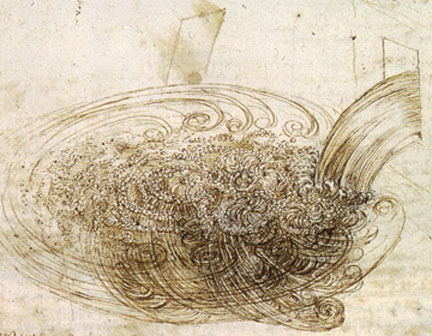
\includegraphics[width=8cm]{AN-Leonardo-Water-Study-723926.jpg}
\legend{Leonardo da~Vinci, \emph{Study of water falling into still water}, c. 1508-9}
\end{center}
Let \(X=[0,1]\times [0,1]\).
A \emph{vector field} \(v\) on \(X\) is a continuous map \(X\xrightarrow{v}\R{2}\).
Picture the vector field as the velocity of a flowing fluid.
We are particularly interested in the points where the vector field vanishes, so a little particle of the fluid does not move.
A vector field is \emph{inward}\define{inward} (or perhaps we should say \emph{not outward}) if the fluid can flow in, but doesn't flow out, of the square \(X\), i.e.\ at each point \(p=(x,y)\in X\), the vector \(v(p)\) doesn't point to the left along the left side, doesn't point up along the top, and so on.
To be more precise, if \(v(p)=(\xi(x,y),\eta(x,y))\), we require that
\begin{align*}
\xi(0,y)&\ge 0 \text{ for all } 0\le y\le 1,\\
\xi(1,y)&\le 0 \text{ for all } 0\le y\le 1,\\
\eta(x,0)&\ge 0 \text{ for all } 0\le x\le 1,\\
\eta(x,1)&\le 0 \text{ for all } 0\le x\le 1.
\end{align*}
A vector field \(v\) is \emph{outward}\define{outward} if \(-v\) is inward.
\begin{theorem}
Every inward or outward vector field on a square vanishes at some point of the square.
\end{theorem}
\begin{proof}
It is enough to prove for inward vector fields, since any outward field \(v\) vanishes just where \(-v\) vanishes.
We can suppose that our square is the unit square \(X=[0,1]\times[0,1]\) and denote our vector field
\[
X\xrightarrow{v}\R{2}.
\]

Suppose that \(v\) has no zero in \(X\), so every point \(p\in X\), \(v(p)\ne 0\).
By compactness of \(X\), we can find some point of \(X\) where \(|v|\) acheives its infimum length, so there is a positive lower bound on \(|v|\), so ther is some \(\varepsilon>0\) so that
\[
|v(p)|>\sqrt{2}\varepsilon>0
\]
for all \(p\in X\).
The reason for putting in a factor of \(\sqrt{2}\) here is that at least one entry of the vector is larger than \(\varepsilon\) in absolute value; to see this, write the entries of \(v\), say \(v(p)=(\xi,\eta)\) and then
\[
\xi^2+\eta^2=|v(p)|^2>2\varepsilon^2,
\]
so at least one of \(\xi^2,\eta^2\) is larger than \(\varepsilon^2\), so at least one of \(|\xi|,|\eta|\) is larger than \(\varepsilon\).

The square \(X\) is compact and \(v\) is continuous, hence \(v\) is uniformly continuous.
By uniform continuity, there is some \(\delta>0\) so that if \(p,q\in X\) have \(|p-q|<\delta\)  then \(|v(p)-v(q)|<\varepsilon\).
Pick some integer \(n\) larger than \(\sqrt{2}/\delta\), so
\[
0<\frac{1}{n}<\frac{\delta}{\sqrt{2}}.
\]

Divide \(X\) into an \(n\times n\) square hex board with small squares of length and height \(1/n\) each.
The center \(p\) of any tile has at least one of \(\xi(p),\eta(p)\) larger than \(\varepsilon\) in absolute value.
Put a white stone on the tile with center \(p\) if \(|\xi(p)|<|\eta(p)|\), i.e. if \(v(p)\) is ``mostly'' pointing up or down, and a black stone otherwise.
We want to see that this hex game has no winner.

Suppose we find a black stone on a tile with center \(p\in X\).
Since the stone is black, \(|\xi(p)|\ge|\eta(p)|\) and so \(|\xi(p)|>\varepsilon\).
We could ask whether \(\xi(p)>\varepsilon\) or whether instead \(\xi(p)<-\varepsilon\), a ``rightward'' or ``leftward'' black stone, i.e. with vector pointing ``mostly'' to the right or to the left.

Claim: if \(p\) and \(q\) are neighboring black stones, we can't have \(p\) rightward, and \(q\) leftward, i.e. we can't have both \(\xi(p)>\varepsilon\) and \(\xi(q)<-\varepsilon\).
Proof: suppose we did.
Because \(p\) and \(q\) are neighbors, they are of distance at most \(\sqrt{2}/n<\delta\), so
\begin{align*}
\varepsilon&>
|v(p)-v(q)|,\\
&\ge
|\xi(p)-\xi(q)|,
\\
&\ge 2\varepsilon
\end{align*}

Using the obvious analogous definitions, an upward white stone upward can't neighbor a downward white stone.
 
Take a path of black stones travelling from left to right.
On the left edge of the square \(X\), \(v\) does not point leftward, so each tile either has a white stone or else \(v\) is rightward and the stone is black.
On the right edge, the vector field does not point rightward, so each tile either has a white stone or \(v\) is leftward and the stone is black.
So our path starts rightward, ends leftward, and so contains a first step from a rightward to a leftward, black stones on neighboring tiles, a contradiction.

The same argument works for a path of white stones travelling from bottom to top.
We conclude that there is no winner in this game of hex, contradicting theorem~\vref{theorem:hex.has.a.winner}.
So finally we contradict our hypothesis that \(v\) vanishes nowhere.
So \(v\) vanishes somewhere.
\end{proof}
The \(n\)-player version of hex proves a similar theorem on the \(n\)-dimensional box, but the notation is too complicated to describe here.
\section{The Brouwer fixed point theorem}
\begin{theorem}[The Brouwer fixed point theorem]
Every continuous map of a square to itself fixes some point of the square.
\end{theorem}
Take two identical pieces of paper%
\SubIndex{paper}
of the same size and shape, one lying directly on top of the other.
Pick up the top piece of paper and crumple it. 
Put it on top of the other piece of paper, so that every point of the crumpled sheet lies above some point of the flat sheet.
Some point of the crumpled piece of paper is now lying exactly on top of the same point of the flat sheet which it was lying on before it was crumpled.
\begin{proof}
We can suppose that our square is the unit square \(X=[0,1]\times[0,1]\) and denote our map
\[
X\xrightarrow{\varphi}X.
\]
The \emph{error vector} of a point \(p=(x,y)\in X\) is \(v_p:=\varphi(p)-p\).
A fixed point is precisely a point \(p\in X\) where \(\varphi(p)=p\), i.e. with vanishing error vector \(v_p=0\).
Each point \(p\) moves under \(\varphi\) to the point \(p+v_p\), i.e. by adding its error vector.
Since no point is carried by \(\varphi\) off of the square, the vector field \(v\) is inward, so has a zero.
\end{proof}
\begin{problem}{brouwer.homeo}
Suppose that \(X\) is a topological space which is homeomorphic to a square.
Prove that every continuous map \(X\to X\) has a fixed point.
\end{problem}
The \(n\)-player version of hex proves a similar theorem on the \(n\)-dimensional box, but the notation is too complicated to describe here.


\end{document}
